\tolerance=10001

\documentclass[12pt]{report}

%This package is built on the LaTeX2e report class, so any other packages which are
%also compatible with it can also be used in combination with it.  ODUthesis should
%be in the directory in which you are working, or in one of the standard input directories
%for the TeX installation on your system.

\usepackage{ODUthesis}
\usepackage{graphicx}
\usepackage{float}

%Use this package and option to label equations, e.g. chapter 1 equation 2 is labeled as (1.2)

\usepackage{amsmath}
\numberwithin{equation}{chapter}

%Use this package to label figures and tables similarly to chapters above

\usepackage[figurewithin=chapter]{caption}

%This allows the use of scalable vector graphics (svg)
%Must use \includesvg{} 
%\usepackage{svg}

%This package causes the first line of a section to be indented as required by the dissertation guide.

\usepackage{indentfirst}

%%%%%Other LaTeX2e packages such as the AMS fonts and graphics packages can be included here.

%This style follows conventions used in Physical Review C. The names of figures, tables and captions can
%be changed by using the commands below with appropriate changes. For example, "FIG." could be replaced by
%"Fig." or "Figure" to change the labeling of figure captions.

%\renewcommand{\figurename}{FIG.}
%\renewcommand{\tablename}{TABLE}
%\renewcommand{\bibname}{BIBLIOGRAPHY}

%%%%%%%%%%%%%%%%%%%%%%%%%%%%
%%%% My Custom Commands %%%%
%%%%%%%%%%%%%%%%%%%%%%%%%%%%

\newcommand{\thetaC}{\theta_{C}} % shortcut for cherenkov angle
\newcommand{\diff}{\mathrm{d}} % differential d for math
\newcommand{\unit}[1]{\text{ #1}}
%\newcommand{\quote}[1]{``#1''}

% Define paths to figures and plots
\graphicspath{{./figures/}{./plots/}}

% Set of commands to allow commenting in bold red
% and listing all comments with page number
% before introductory chapter
\usepackage{tocloft}
\newcommand{\listcomments}{Comments}
\newlistof{comments}{comm}{\listcomments}
\newcommand{\comment}[1]{%
	\refstepcounter{comments}%
	\textbf{\large \pdfliteral{1 0 0 rg} #1 \pdfliteral{0 0 0 rg}}%
	\addcontentsline{comm}{comments}{{\large \pdfliteral{1 0 0 rg} #1 \pdfliteral{0 0 0 rg}}}
} % add big colored comment to text so it's easily identified later

\begin{document}

\title{R\&D of a High-Performance DIRC Detector for use in an Electron-Ion Collider}

\author{S. Lee Allison}
\principaladviser{Charles Hyde}
\member{Gagik Gavalian}
\member{Mark Havey}
\member{Grzegorz Kalicy}  %This command produces a signature line for the specified member on the
\member{Jay Van Orden}
\member{Mike Overstreet}  %title page. Use on instance of this command for each member of the
                   %committee other than the advisor up to a total of 5 members.

\degrees{MS in Physics}

\dept{Physics}          %for example \dept{physics}

\submitdate{May 2017}

%\phdfalse          %produces language on title page for Masters Thesis. 
                    %otherwise the default is for a Ph.D. dissertation.

%\copyrightfalse    %suppresses copyright notice

%\figurespagefalse  %suppresses List of Figures

%\tablespagefalse   %suppresses List of Tables

\vita{The text of the Vita goes here.}


\abstract{text of abstract goes here}

\beforepreface

\prefacesection{Acknowledgements}

    %text of Acknowledgements goes here, any other preface section is inserted similarly by the command \prefacesection{Section Title}

\afterpreface

\listofcomments

    %The text of the thesis/dissertation begins here. The basic organization is in chapters, sections, subsections. 

\chapter{Introduction}
%----------------------------------------------------------------------
%	INTRODUCTORY CHAPTER
%----------------------------------------------------------------------
\label{ch:intro} % intro, eic, etc
%
\chapter{Electron-Ion Collider}
%-------------------------------------------------------------------------------
%	EIC CHAPTER
%-------------------------------------------------------------------------------
\label{ch:eic}
It has been known for nearly a century that atoms are composed of nucleons (protons and neutrons), but it took another 50 years for Murray Gell-Mann and George Zweig to independently develop a model proposing that nucleons themselves are made up of constituent components, called quarks, bound together by the exchange of gluons \cite{SLACquark}. This lead to the development of the fundamental theory of the strong interaction, known as Quantum Chromo-Dynamics (QCD). It is now a strong goal of the nuclear physics community to understand the interactions of quarks and gluons and how those interactions make manifest both nucleons themselves, which account for nearly all the mass of the visible matter in the universe, as well as the nucleons' spin, mass, magnetic moment, and nuclear binding energy. Because of the well-known properties of the electromagnetic interaction, electron scattering is an ideal process for such studies. 

Although it would theoretically be possible to study these properties using fixed-target electron beam experiments, it is three-fold prohibitive: it is much more costly to construct an accelerator to accelerate electrons to the necessary momentum (on the order of TeV) than to build a collider, it is more difficult and complicated to do transverse nucleon polarization studies with a fixed target due to the nature of the required magnetic fields, and it is very difficult to study the target fragments of a fixed target reactions due to final state interactions whereas in a collider the fragments will be boosted in the same direction as the ion beam. It was therefore deemed a priority by the 2007 Nuclear Science Advisory Committee's Long-Range Plan that an Electron-Ion Collider (EIC) be the next facility to be built in the United States \cite{NSAC2007}.

The EIC will not be the first facility to have the capability of colliding electrons and positrons with protons. The HERA accelerator in Hamburg, Germany was the world's first electron-proton collider, reaching electron energies of up to 28 GeV and protons to nearly 1 TeV with a luminosity on the order of $10^{31}\unit{cm}^{-2}\unit{s}^{-1}$ before shutting down in 2007. Figure \ref{fig:HERA_pdf} shows the combined H1 and Zeus experimental data from HERA for the measurement of the structure function for positron-proton scattering along with fixed target data for a wide range of both $x$ and $Q^2$. The EIC hopes to improve upon the already rich science produced at HERA threefold: by increasing the luminosity of the accelerator to on the order of $10^{34}\unit{cm}^{-2}\unit{s}^{-1}$, by allowing for the use of heavier ion beams such as oxygen, and by allowing for both transversely and longitudinally polarized beams of electrons and light ions. With these improvements the EIC will be able to look into hadronic final states with much greater detail.

\begin{figure}[ht]
	\centering
	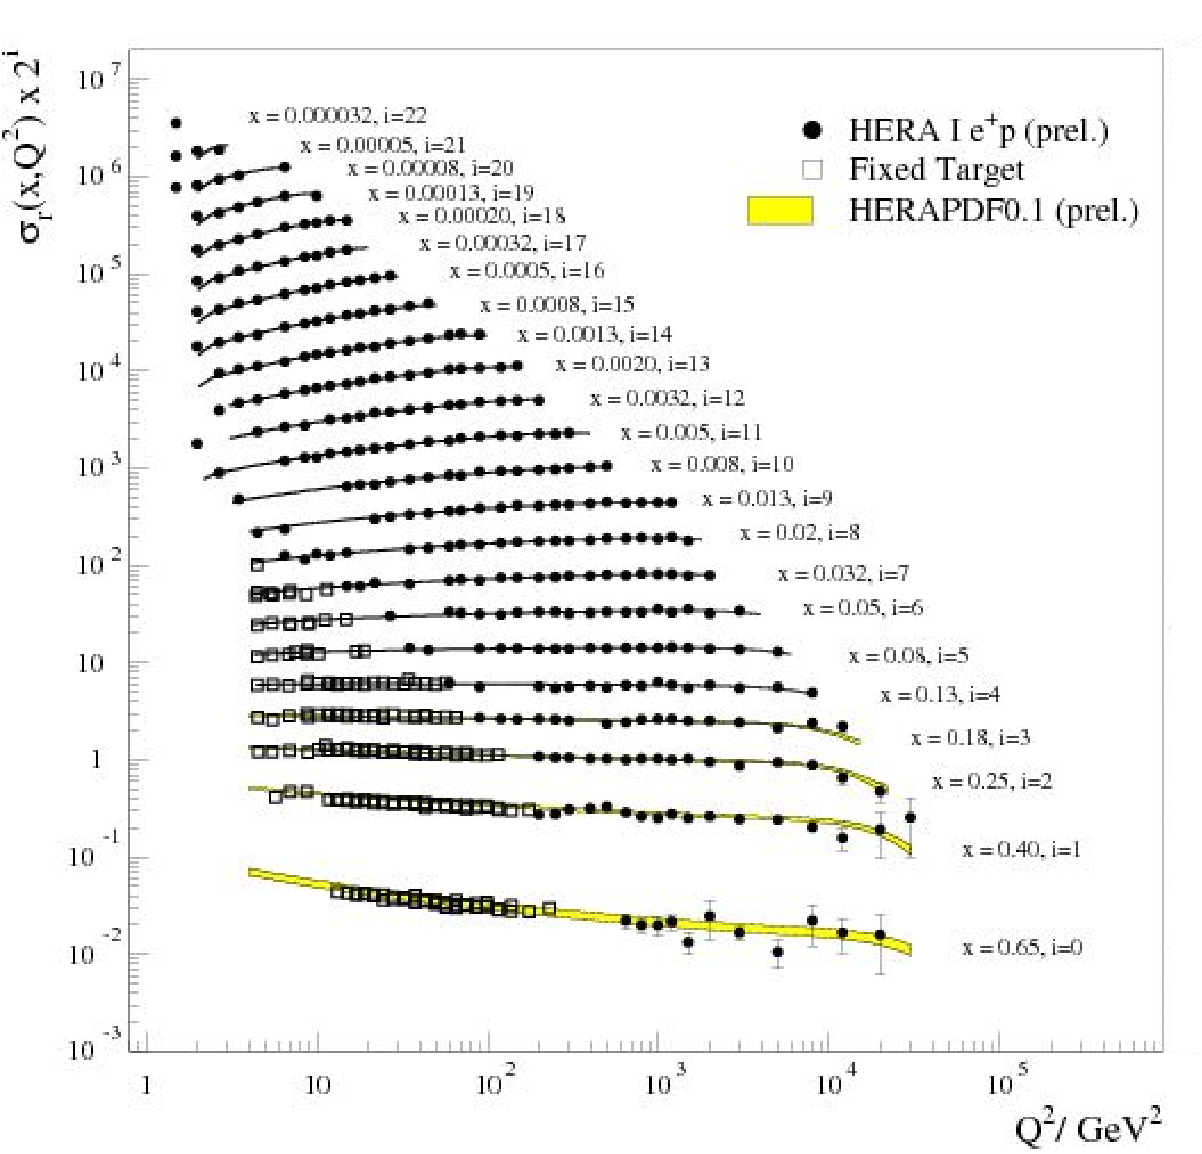
\includegraphics[scale=0.7]{HERA_PDF.pdf}
	\caption{The reduced cross section $\sigma_{r}(x,Q^2)$ as a function of $Q^2$. Filled circles are combined H1 and Zeus data from HERA for proton-positron collisions, hollow squares are from fixed target experiments, and the yellow is prediction from HERAPDF0.1}
	\label{fig:HERA_pdf2}
\end{figure}

%-------------------------------------------------------------------------------
%	SCIENCE GOALS SECTION
%-------------------------------------------------------------------------------
\section{Science Goals}
The goal of an EIC will be to find out how QCD is responsible for the structure and dynamics of nucleons, the nature of the nucleon-nucleon force, and the relative importance of the valance quarks.

\subsection{Nucleon Spin}
One major question still pestering nuclear physicists is ``What is the origin of the nucleon spin?''. In the 1980s the naive answer was that the total nucleon spin was the sum of the spin of its three valance quarks, but many years of experimentation has revealed that it is much more complicated (Fig. \ref{fig:nucleon_spin}), with the contributions from gluons and orbital angular momentum still in question. The EIC will be capable of much more detailed study of the contributions to the nucleon structure by enabling multi-dimensional projections of the distribution of quarks and gluons in space, longitudinal and transverse momenta, spin, and flavor.

\begin{figure}[ht]
	\centering
	\includegraphics[scale=.08]{nucleon_spin.png}
	\caption{Evolution of our understanding of nucleon spin structure. \textbf{Left:} In the 1980s, a nucleon’s spin was naively explained by the alignment of the spins of its constituent quarks. \textbf{Right:} In the current picture, valence quarks, sea quarks and gluons, and their possible orbital motion are expected to contribute to overall nucleon spin.}
	\label{fig:nucleon_spin}
\end{figure}

\subsection{The EMC Effect}
It was first observed by the European Muon Collaboration (EMC), and confirmed by other experiments that there is a modification between the nucleon structure function, $F_2$, of deuterium to those of heavier elements as a function of Bjorken $x$ \cite{SRC_EMC_effect}. Figure \ref{fig:emc_effect} shows the ratio of structure functions of Carbon and Deuterium for $x$ between $0.2$ and $0.9$. Initial assumptions were that this ratio of structure functions would be unity, but measurements have clearly shown a suppression in this ratio for $x$ values between $0.3$ and $0.8$.

\begin{figure}[ht]
	\centering
	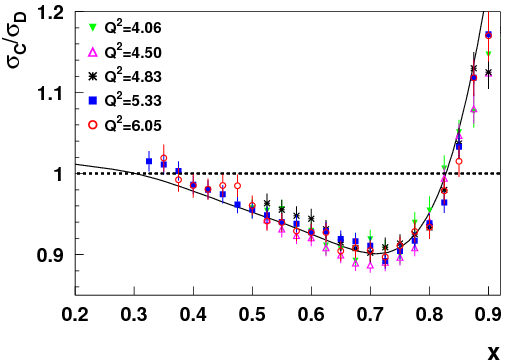
\includegraphics[scale=0.85]{emc_effect.png}
	\caption{Ratio of the nucleon structure functions for Carbon and Deuterium for $x$ between $0.2$ and $0.9$ and a range of $Q^2$ values.}
	\label{fig:emc_effect}
\end{figure}

The reason for this modification to the nuclear structure function is still a mystery, but the EIC hopes to shed light on this phenomenon by studying various coherent exclusive reactions, such as $J/\Psi$ production, which could allow for the quantification of initial conditions in heavy-ion collisions by mapping out the geometry of the nucleus in high-energy processes. This mapping can also help to understand other collective dynamics, such as shadowing and anti-shadowing.

\subsection{Gluon Distributions Inside Nuclei}
As mentioned above, the EMC effect, the modification of the distribution of quarks in a nucleus versus their distribution in nucleons, is a known (yet still mysterious) phenomenon. It is suspected that this modification also occurs for gluons, with experiments such as ALICE showing evidence for gluon shadowing for $x \approx 10^{-3}$ \cite{ALICE_antishadowing}. The EIC hopes to measure this suppression of the structure functions thanks to its wider range of kinematics both in $x$ and $Q^2$, allowing not only for the measurement of gluon shadowing ($x < 0.05$), but also anti-shadowing ($x \approx 0.1$), and possibly the EMC effect for gluons ($x > 0.3$), shedding light on the origins of the EMC effect.

%-------------------------------------------------------------------------------
%	FACILITIES SECTION
%-------------------------------------------------------------------------------
\section{Facilities}
As of the writing of this thesis there are two competing designs for an EIC facility to be built in the United States: a figure-8 accelerator design for Thomas Jefferson National Accelerator Facility (JLab) (Figure \ref{fig:jleic_layout}), and a ring-ring accelerator design for Brookhaven National Lab (BNL) (Figure \ref{fig:erhic_layout}).

\begin{figure}[ht]
	\centering
	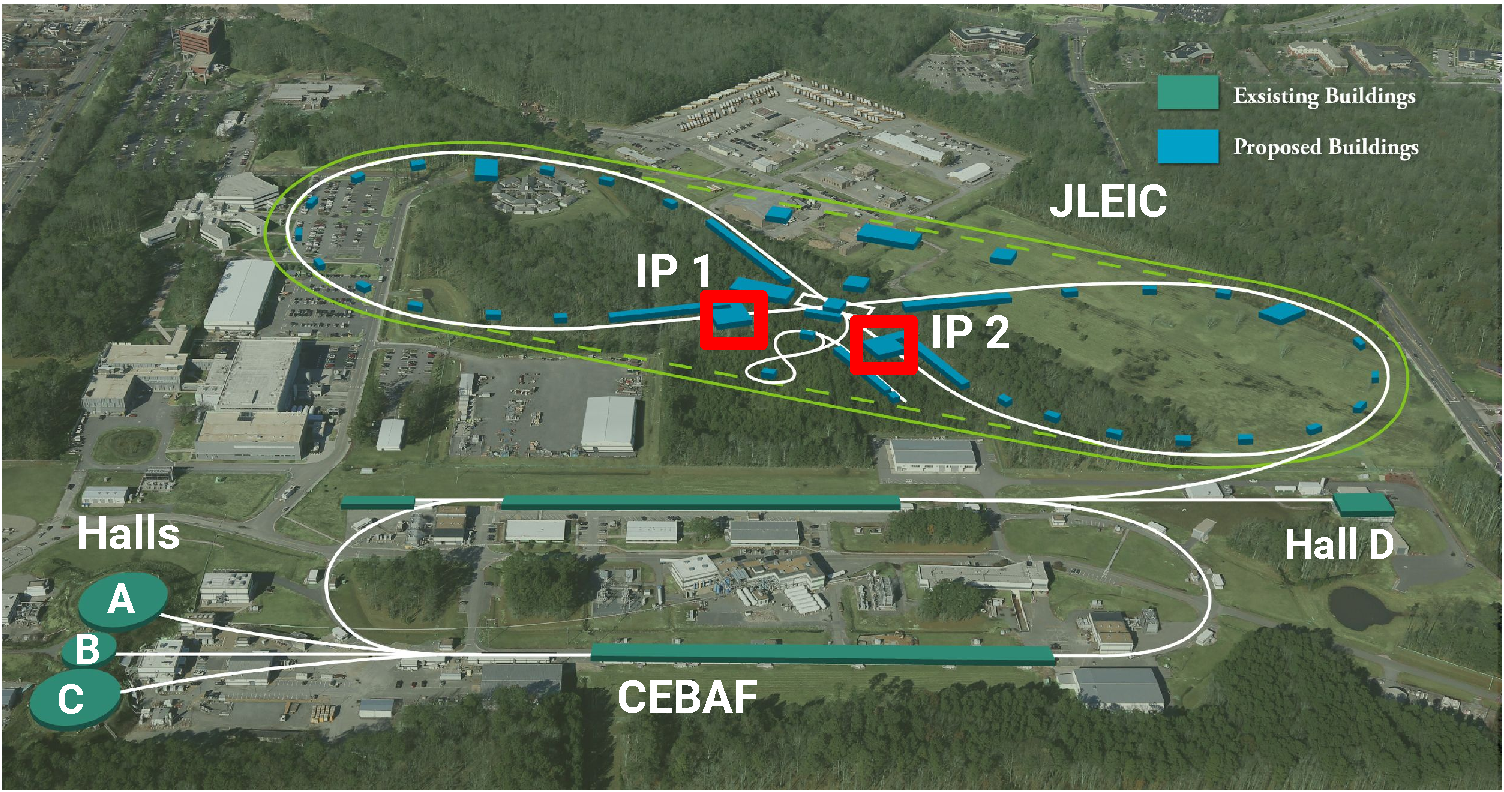
\includegraphics[scale=0.5]{JLEIC_layout2.pdf}
	\caption{Current design of the EIC facility for JLab with the two interaction points highlighted in red.}
	\label{fig:jleic_layout}
\end{figure}

\begin{figure}[ht]
	\centering
	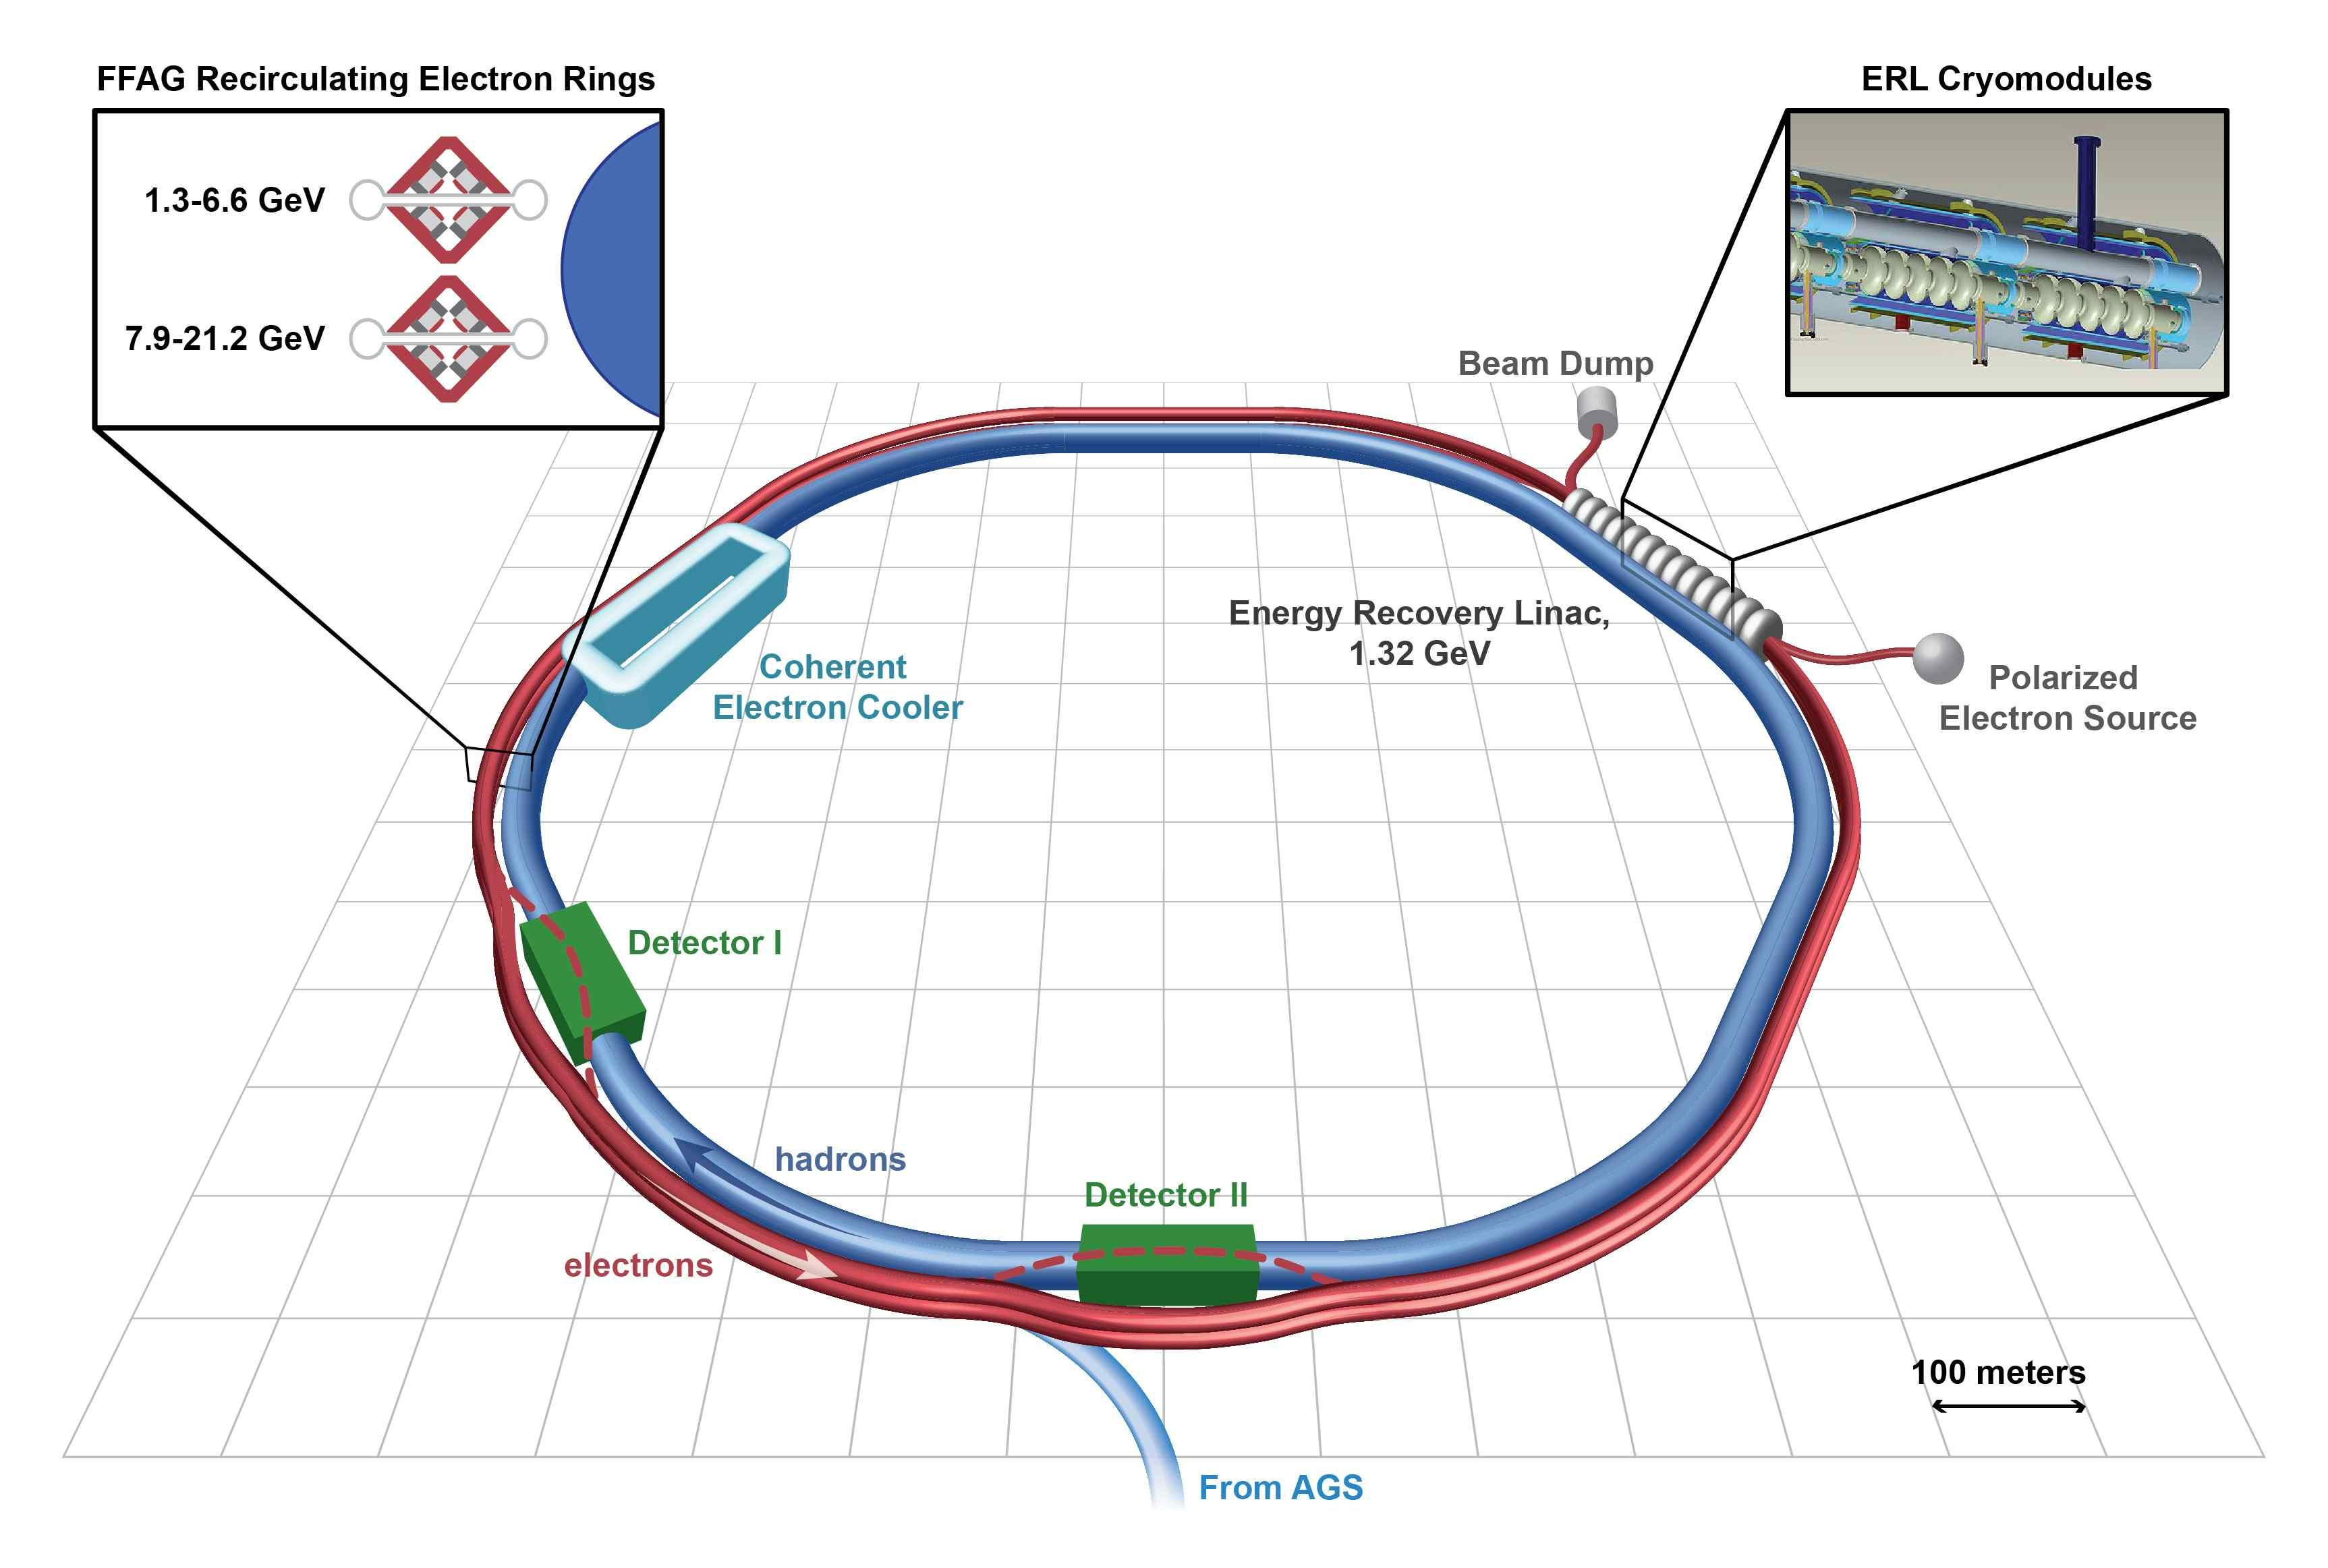
\includegraphics[width=\textwidth]{eRHIC_Layout.jpeg}
	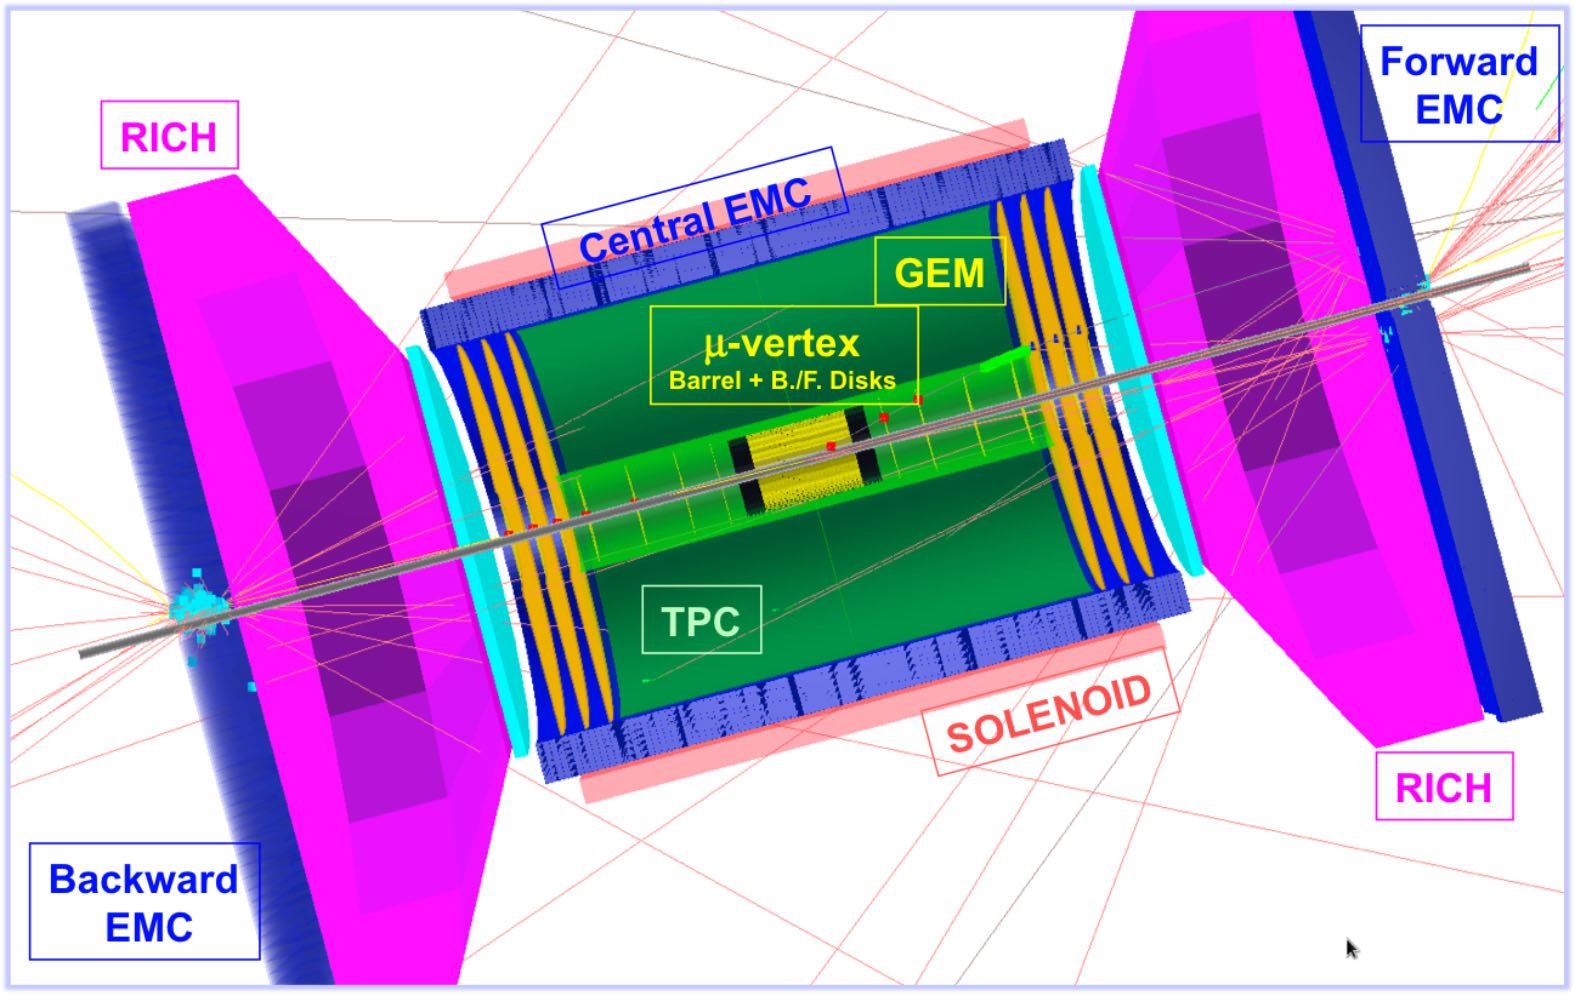
\includegraphics[width=\textwidth]{eHRIC_beast.png}
	\caption{Current design of the EIC facility at BNL (top), and the proposed BeAST (Brookhaven eA Solenoidal Tracker) detector (bottom).}
	\label{fig:erhic_layout}
\end{figure}

The JLab EIC (JLEIC) is planned to be approximately 1.4 km in circumference and have a footprint of roughly 500 m by 170 m. The design is a ring-ring with electrons and ions being stored in separate beam lines and collided at two interaction points  (IPs) (outlined in red in Figure \ref{fig:jleic_layout}) on the figure-8. The JLab CEBAF SRF linac will be used as an electron injector for electrons with 3 - 11 GeV energy. The second ring will store an ion beam with energy of 20 to 100 GeV for protons or up to 40 GeV per nucleon for light to heavy ions. The ion beams are generated and accelerated in a new ion injector complex with the same figure-8 design that will be utilized to preserve ion polarization. The two rings will be stacked vertically in the same underground tunnel \cite{JLEICdesign}.

The BNL facility, named eRHIC, will use a new electron beam facility based on an Energy Recovery LINAC that will be built inside of the Relativistic Heavy Ion Collider (RHIC) tunnel to collide with RHIC's pre-existing polarized proton/ion beam. The existing hadron ring will accelerate protons up to 250 GeV/c, $^3$He$^{+2}$ up to 167 GeV/c per nucleon, and heavier ions (e.g. gold or uranium) up to 100 GeV/c per nucleon. The new electron ring will be capable of producing electrons from 2 - 21 GeV/c \cite{eRHICdesign}.

%-------------------------------------------------------------------------------
%	JLEIC DETECTOR SECTION
%-------------------------------------------------------------------------------
\subsection{JLEIC Detector Design}
The large center of mass energies and diverse physics program at an EIC necessitate a very sophisticated detector system. Figure \ref{fig:jleic_detector} shows the current design of the JLab EIC detector at IP1. This 

\begin{figure}
	\centering
	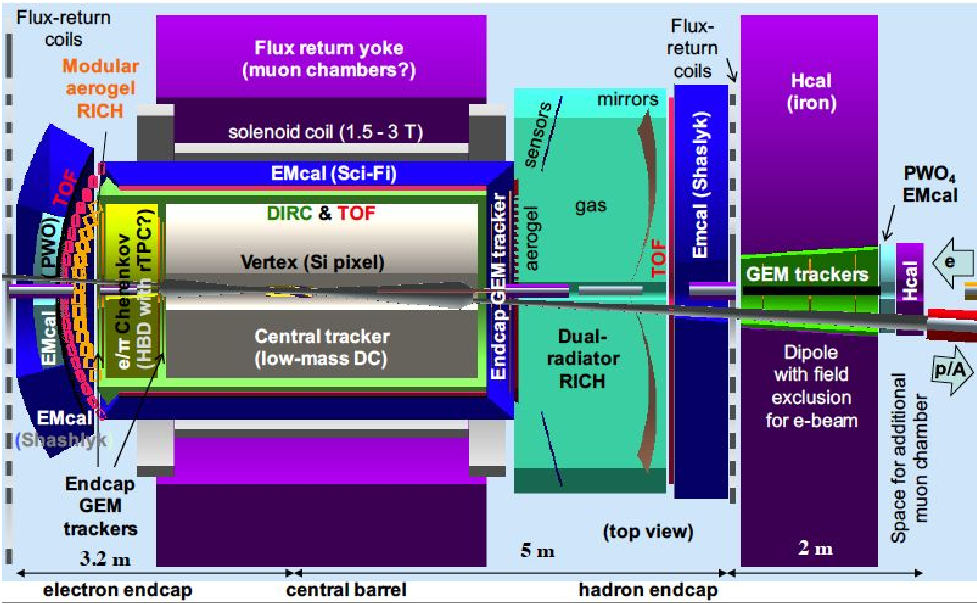
\includegraphics[scale=1]{JLEIC_detector.pdf}
	\caption{Current design of the detector to be used in the JLab EIC at IP1}
	\label{fig:jleic_detector}
\end{figure}

%-------------------------------------------------------------------------------
%	PARTICLE ID SUBSECTION
%-------------------------------------------------------------------------------
\subsection{Particle Identification}
The ability to accurately identify hadrons in the final state is a key requirement for the physics program at an EIC. % description of EIC and why it's needed
%
\chapter{DIRC Technology}
%-------------------------------------------------------------------------------
%	DIRC TECHNOLOGY CHAPTER
%-------------------------------------------------------------------------------
\label{ch:dirc}
DIRC detectors are based on the concept of the Detection of Internally Reflected Cherenkov light (DIRC) produced in a solid radiator bar to identify charged particle. It is a special type of Cherenkov counter, which uses the unique properties of Cherenkov radiation to identify charged particle species.

%-------------------------------------------------------------------------------
%	CHERENKOV RADIATION SECTION
%-------------------------------------------------------------------------------
\section{Cherenkov Radiation}
Einstein postulated in his Theory of Relativity that the speed of light in a vacuum, $c$, is the limit of the velocity of massive particles. In an optically transparent medium, however, the speed at which light propagates is modified: $c_{med} = c/n$, where $n$ is the index of refraction of the medium. Pavel Cherenkov discovered in 1934 that massive particles moving through a medium faster than the speed of light in that medium emit light in the form of now-called Cherenkov radiation. Cherenkov was able to establish several interesting properties of this radiation: it is only emitted from charged particles above a certain velocity threshold $v > c/n$, the intensity is proportional to the particle's path length, emission is prompt, and the light is polarized with a continuous wavelength spectrum. Later in 1937 Ilya Frank and Igor Tamm theoretically formulated this radiation with fantastic agreement to Cherenkov's findings, and the three shared the 1958 Nobel Prize in Physics for their efforts \cite{CherenkovHistory}.

Further studies confirmed that Cherenkov radiation is emitted uniformly in azimuth ($\phi_c$) around the particle's direction of travel with the polar opening angle $\thetaC$ defined as

\begin{equation}
	\cos\thetaC = \frac{1}{\beta n(\lambda)},
	\label{eq:cherenkovformula}
\end{equation}

where $\beta = v_p/c$, $v_p$ is the particle's velocity, and the index of refraction is a function of the emitted photon wavelength. In a normal, dispersive optical medium the opening half-angle of the shock wave produced by the Cherenkov radiation, $\eta_C$ defined in Figure \ref{fig:cherenkovcone}, is not complementary to the Cherenkov angle. The relationship between the two is given by

\begin{equation}
	\cot\eta_C = \left[\frac{\diff}{\diff\omega}(\omega \tan\thetaC) \right]_{\omega_0} = \left[\tan\thetaC + \beta^2\omega n(\omega) \frac{\diff n}{\diff\omega}\cot\thetaC \right]_{\omega_0}
	\label{eq:openingangle}
\end{equation}

where $\omega_0$ is the central vale of the considered frequency range. Because the second term in (\ref{eq:openingangle}) is zero only for non-dispersive media the shock wave front is not perpendicular to the Cherenkov cone in real detectors.

\begin{figure}[ht]
	\centering
	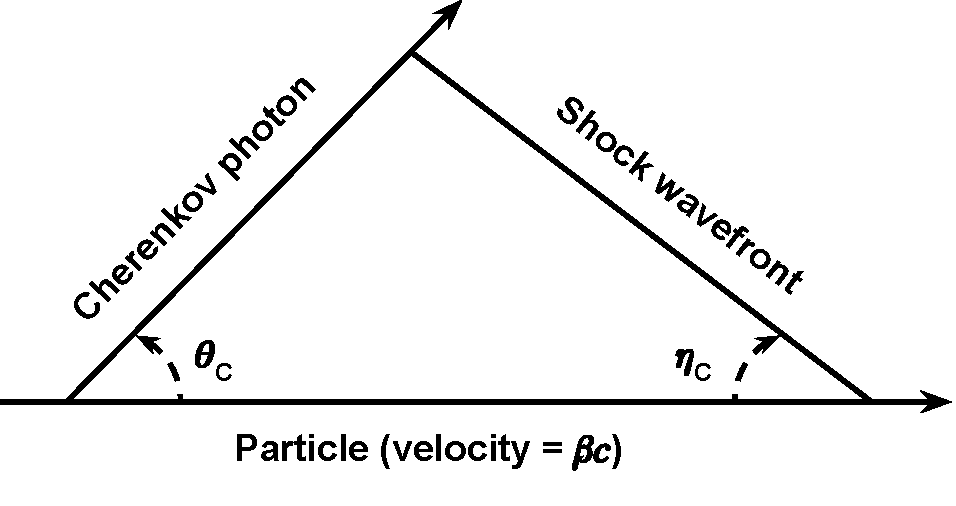
\includegraphics[scale=1]{Cherenkov_cone.pdf}
	\caption{Illustration of the Cherenkov cone.}
	\label{fig:cherenkovcone}
\end{figure}

Because particles lose very little energy when radiating Cherenkov photons the emission is very weak. The number of photons $N_{photons}$ emitted per path length $L$ (in cm) by a moving particle with charge $z$ is given by the Frank-Tamm equation

\begin{equation}
	\frac{N_{photons}}{L} = \frac{\alpha^2 z^2}{r_e m_e c^2} \int \sin^2\thetaC (E) \diff E
	\label{eq:nphotons}
\end{equation}
where E is the photon energy in eV, the integral is taken over the region where $n(E)$ is greater than 1, and $\frac{\alpha^2 z^2}{r_e m_e c^2} = 370\unit{cm}^{-1}\unit{eV}^{-1}$.

%-------------------------------------------------------------------------------
%	APPLYING TO PID SECTION
%-------------------------------------------------------------------------------
\section{Applying the Cherenkov Effect to Particle ID}
In order to identify particle species one must know both the mass and charge of the particle in question. Because the Cherenkov angle encodes the particle's velocity it is, in principle, a simple matter to measure the particle's momentum with a tracking chamber as well as the velocity obtained from (\ref{eq:cherenkovformula}) to determine the mass and charge. Figure \ref{fig:angleseperation} shows how different particle species can be distinguished for a given momentum in fused silica.

Threshold Cherenkov counters are detectors used for particle identification (PID) by exploiting the fact that only particles above the threshold velocity $\beta > 1/n$ will emit Cherenkov photons. The information about a particle's velocity can be combined with momentum information from a tracking system to determine the mass as \cite{ParticleDetectionHandbook}

\begin{equation}
	m = \frac{p}{c} \sqrt{n^2 \cos^2\thetaC - 1}
	\label{eq:mass}
\end{equation}

\begin{figure}[ht]
	\centering
	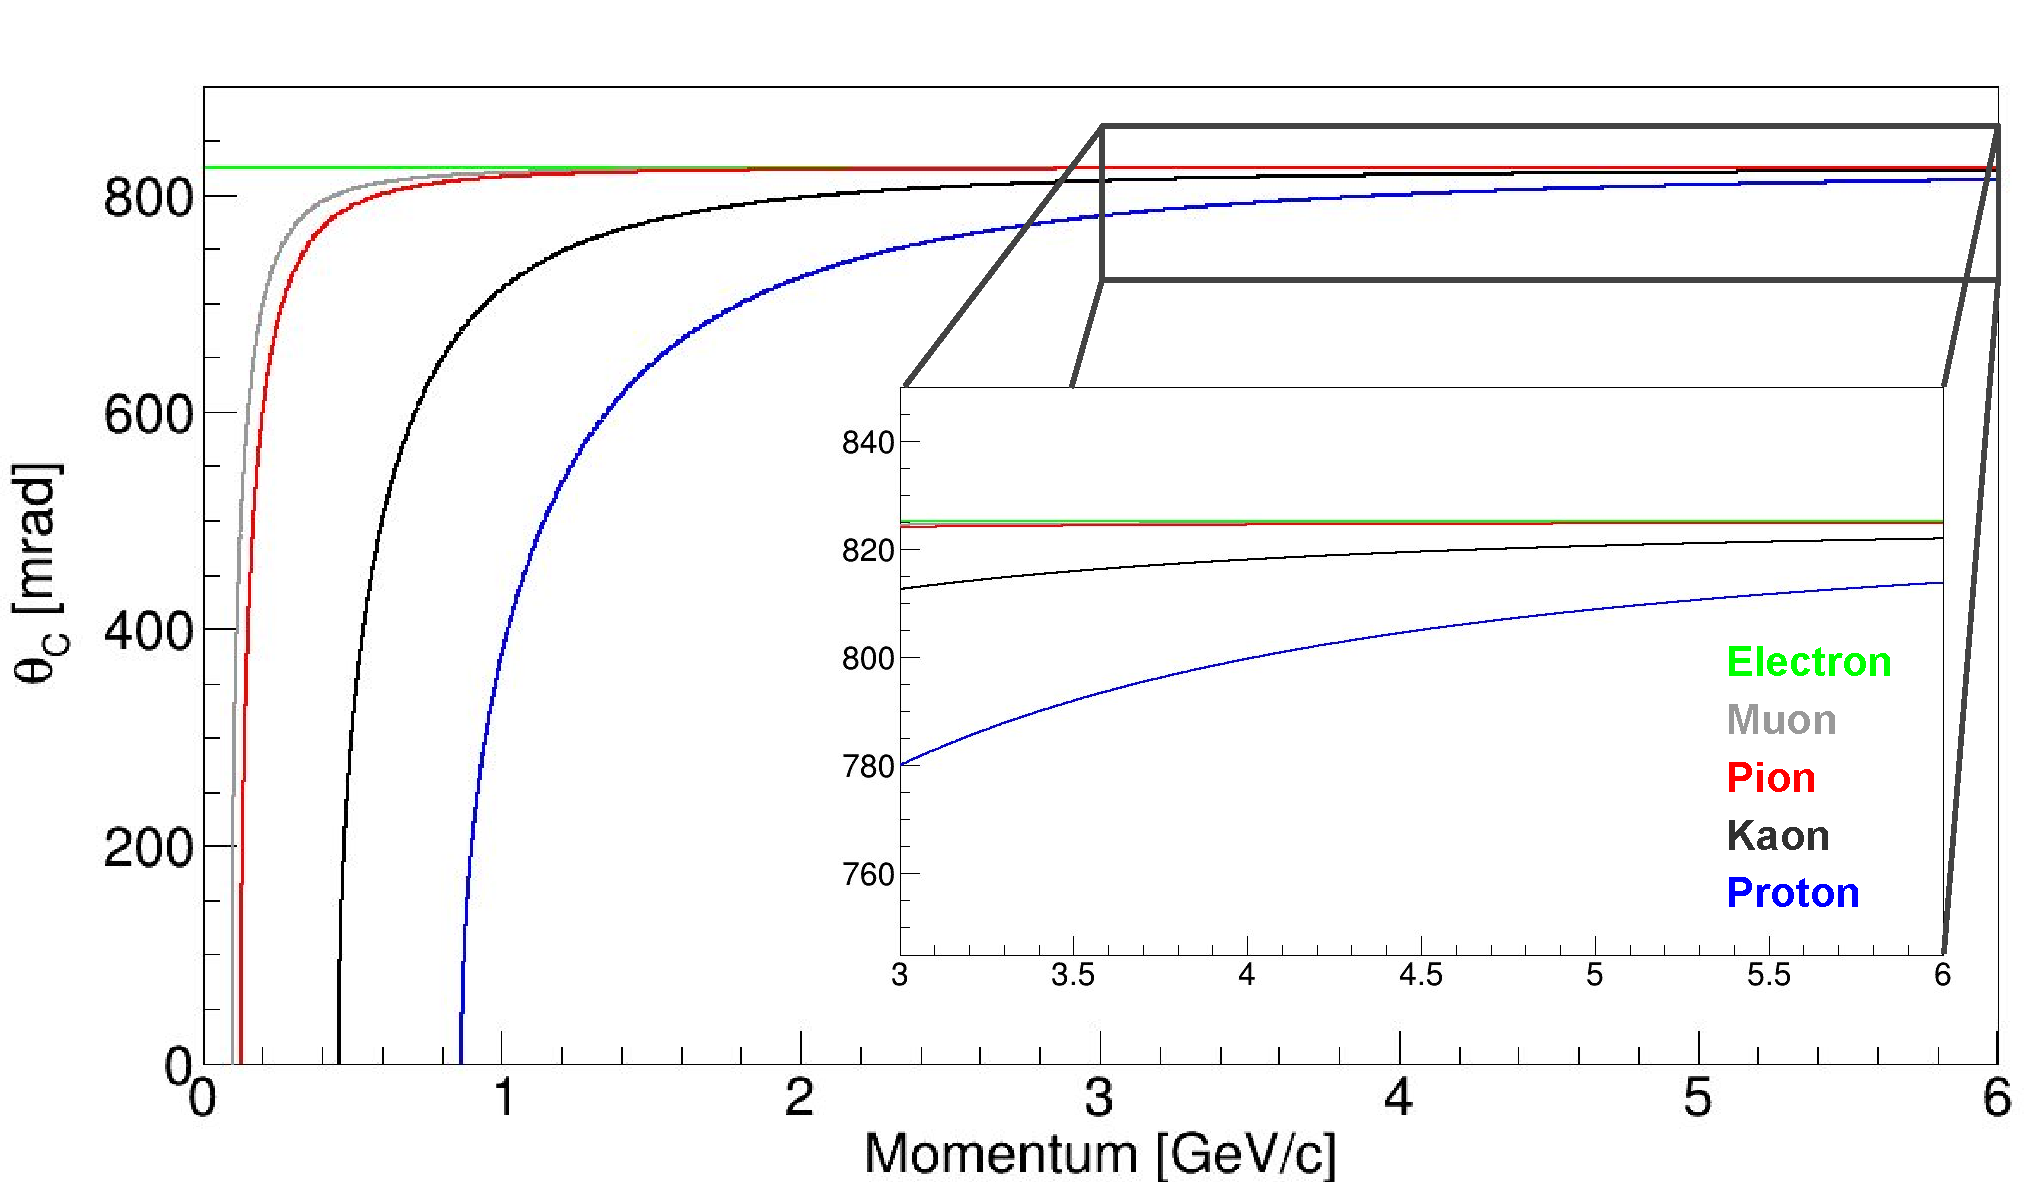
\includegraphics[width=\textwidth]{angle_seperation_enhance.pdf}
	\caption{Particle momentum [GeV/c] versus Cherenkov angle [mrad] for different particle species in fused silica ($n \approx 1.473$). The zoomed image shows that it is indeed possible to differentiate pions, kaons, and protons at higher particle momenta.}
	\label{fig:angleseperation}
\end{figure}

%-------------------------------------------------------------------------------
%	RICH SECTION
%-------------------------------------------------------------------------------
\section{Ring Imaging Detectors}
Ring Imaging Cherenkov (RICH) detectors are designed to efficiently identify and separate different particle species over a wide range of momenta. A basic RICH system is shown in Figure \ref{fig:rich_basics}. 

\begin{figure}[ht]
	\centering
	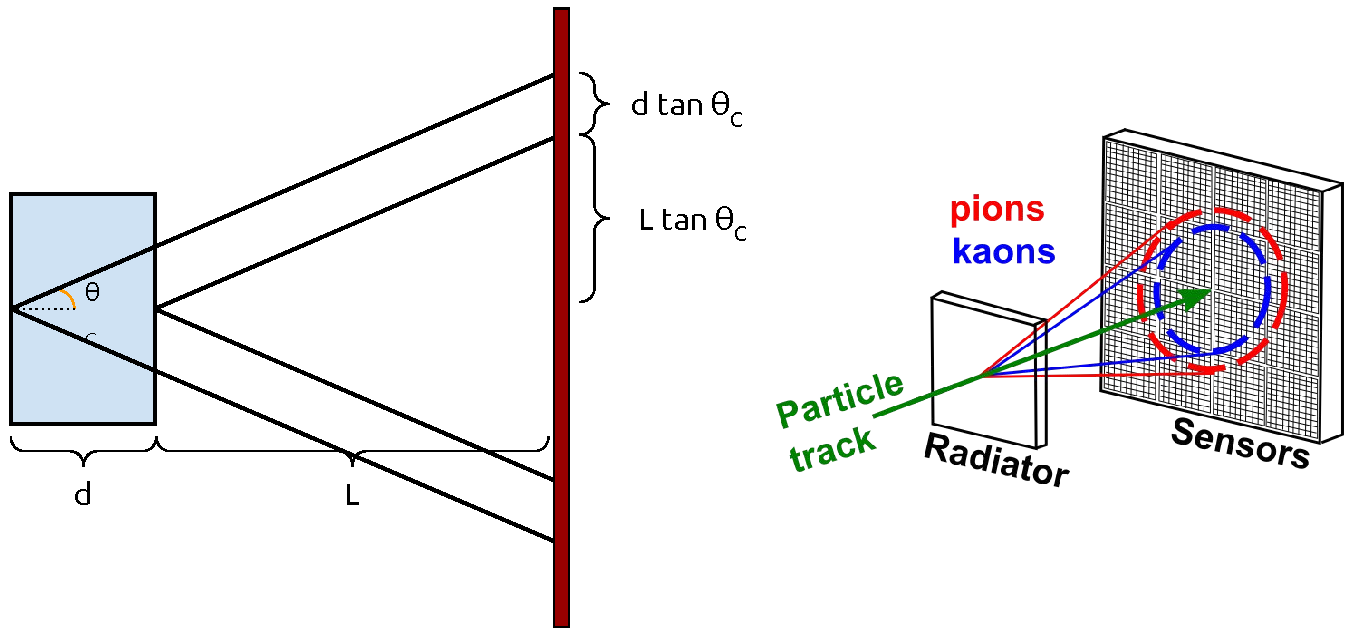
\includegraphics[width=\textwidth]{RICH_rings.pdf}
	\caption{Basic concept of a proximity focusing Ring Imaging Cherenkov (RICH) detector (a), and an example of how they can be used to do PID based on particle mass (b).}
	\label{fig:rich_basics}
\end{figure}

A volume of radiator, either gaseous (e.g. $C_{4}F_{10}$) or solid (e.g. aerogel), is positioned upstream of an array of photosensors. A charged particle traveling through a thin radiator above the threshold velocity will continuously emit Cherenkov photons in a cone. The resulting image on the photosensor array is an annulus of thickness $d\tan\thetaC$ and an inner radius of $L\tan\thetaC$, where $d$ is the distance the particle traveled inside the radiator, $L$ is the distance between the radiator and the photsensors, and  $\thetaC$ is the usual Cherenkov angle (Figure \ref{fig:rich_basics}b). PID is done by measuring the average radius of the annulus and reconstructing the Cherenkov angle geometrically.


%-------------------------------------------------------------------------------
%	DIRC SECTION
%-------------------------------------------------------------------------------
\section{DIRC Detectors}
DIRC detectors work much the same way as a RICH in that collect Cherenkov photons produced from a radiating material and use the created image on the photosensors to reconstruct the Cherenkov angle. In the case of a DIRC, the radiating medium is also used as a light guide as some of the Cherenkov photons undergo total internal reflection inside the radiator and are guided towards one end of the radiator to a readout (Figure \ref{fig:dircbasics}). The radiator of choice is a solid bar made of fused silica, with an index of refraction $n \approx 1.473$. A rectangular cross section and highly smoothed and polished sides ensure that the magnitude of the Cherenkov angle is preserved during internal reflection. Photons that are created propagating away from the readout are reflected back towards the readout by a mirror. Once the photons exit the radiator they are allowed to separate through an expansion volume before being imaged in both ($x, y$) position as well as time. The arrival position and propagation time of each detected photon are combined with tracking information to reconstruct the Cherenkov angle and determine the corresponding PID likelihoods (reconstruction methods and techniques for DIRC detectors will be discussed in detail in Chapter \ref{ch:analysis}).

\begin{figure}[ht]
	\centering
	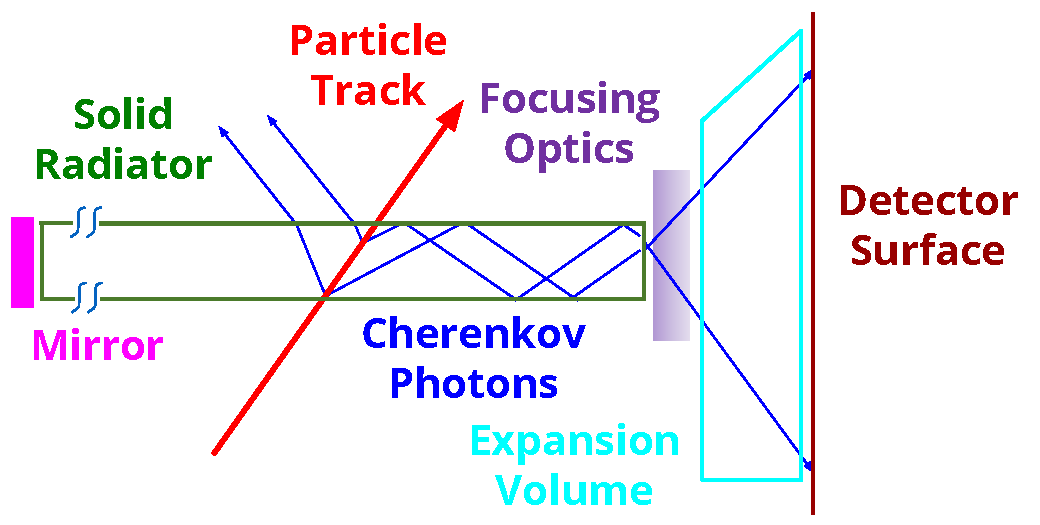
\includegraphics[scale=0.7]{DIRC_components.pdf}
	\caption{The basic components of a DIRC detector: a solid radiator, typically fused silica (green); a mirror to redirect backward-going photons (pink); optional focusing optics (purple); an expansion volume to allow photons to separate in space (cyan); and a detector surface to record the position and arrival time of Cherenkov photons (maroon).}
	\label{fig:dircbasics}
\end{figure}

The performance of a DIRC detector is given by the resolution in the Cherenkov polar opening angle of the particle track, $\sigma_{\thetaC,\text{track}}^2$, which can be written as:

\begin{equation}
	\sigma_{\thetaC,\text{track}}^2 = \sigma_{\thetaC}^2 / N_{\gamma} + \sigma_{\text{correlated}}^2
	\label{eq:performance}
\end{equation}

where $\sigma_{\thetaC}$ is the average single photon Cherenkov angle resolution, $N_{\gamma}$ is the number of measured photons per track, and $\sigma_{\text{correlated}}$ includes several correlated terms that contribute to the resolution such as the uncertainty in the particle track direction coming from external tracking systems. Because the track direction is crucial to the reconstruction of the Cherenkov angle, this error needs to be small for the performance to not suffer. For the EIC a tracking resolution on the order of 1 mrad is required for adequate PID.

\begin{figure}[ht]
	\centering
	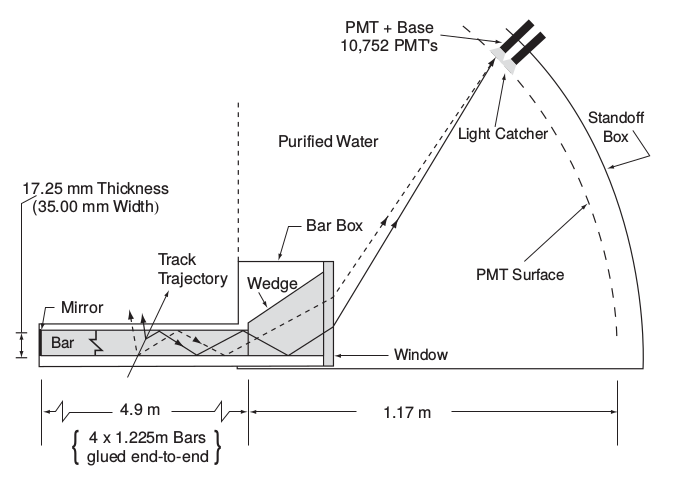
\includegraphics[width=\textwidth]{BaBar_DIRC.png}
	\caption{Schematic of BaBar DIRC and imaging region.}
	\label{fig:babardirc}
\end{figure}

As of the writing of this thesis the only DIRC detector used in a full experiment is the BaBar DIRC at SLAC National Accelerator Laboratory, which was successfully operated from 1999 through 2008 \cite{BaBarDIRC}. It proved to be a robust, stable, and easy to operate system for more than 8 years, providing excellent pion/kaon separation for all tracks from $B$-meson decays. It used 4.9 m long radiator bars with a rectangular cross section of $17.25 \times 35 \unit{mm}^2$. Each bar was made of four $1.225\unit{m}$ long fused silica bars glued end-to-end. The bars were placed in 12 hermetically sealed containers, called bar boxes, each holding 12 radiator bars for a total of 144 bars. At the end of each box was attached a wedge of fused silica and a window to allow the photons to expand before entering the water-filled expansion volume and being read out on one of 10,752 photomultiplier tubes (see Figure \ref{fig:babardirc}). Figure \ref{fig:babarperformance} summarizes the performance of the BaBar DIRC, showing excellent Cherenkov angle reconstruction (2.5 mrad, only 14\% larger than the design goal of 2.2 mrad) and photon yield per track.

\begin{figure}[ht]
	\centering
	a)%
	\raisebox{-1.0\height}{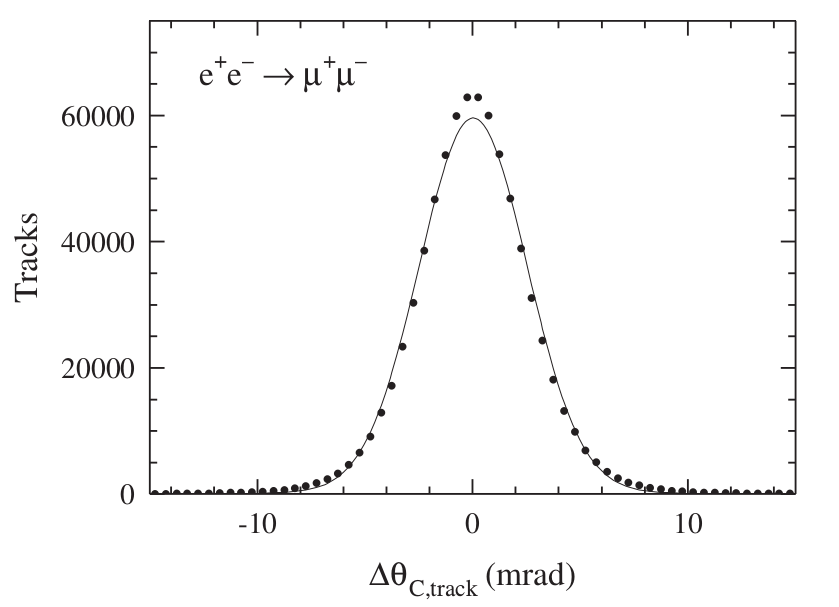
\includegraphics[width=0.5\textwidth]{BaBar_SPR.png}}%
	b)%
	\raisebox{-1.0\height}{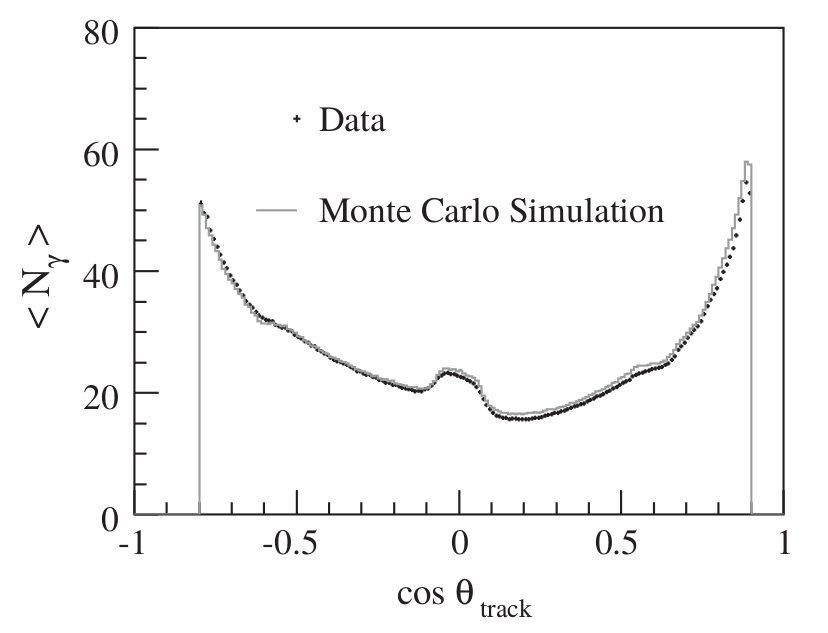
\includegraphics[width=0.5\textwidth]{BaBar_NPH.png}}
	\caption{Performance of the BaBar DIRC for $e^{+}e^{-} \rightarrow \mu^{+}\mu^{-}$ events. a) shows the difference between the measured and expected Cherenkov angle (dots) and a Gaussian fit to the data with a 2.5 mrad width (line). b) is the average number of detected photons vs. track polar angle for data (dots) and Geant4 simulation (line).}
	\label{fig:babarperformance}
\end{figure}

\subsection{DIRCs in Future Experiments}
The BaBar DIRC has since inspired many other experiments/facilities, including the EIC, to utilize this new, novel PID system in a variety of ways (Figure \ref{fig:dirc_evolution}). The Focusing DIRC (FDIRC) proposed for the now-cancelled SuperB collider in Italy was the first to propose using some form of focusing for the Cherenkov photons, allowing for a factor of 10 smaller expansion volume \cite{FDIRC}. The barrel DIRC for the PANDA experiment at FAIR in Germany will use shorter radiator bars for a more compact design \cite{PANDA_barrel}, while the PANDA disc DIRC will be used in the forward region and will be the first disc DIRC to be used in a high-performance $4\pi$ detector \cite{PANDA_disc}. Belle II at the SuperKEKB accelerator in Japan will utilize wide plates as radiators and focus on fast timing for PID in the barrel region \cite{Belle2_TOP}. The TORCH detector, similar to the PANDA disc DIRC, will be a large-area detector focusing on precision time-of-flight to do PID for low momentum kaons at the upgraded LHCb experiment \cite{TORCH}. The GlueX experiment at JLab will be recycling four bar boxes from the BaBar experiment to cover the forward region of their spectrometer; utilizing  focusing similar to the FDIRC design \cite{GlueX}.

\begin{figure}[ht]
	\centering
	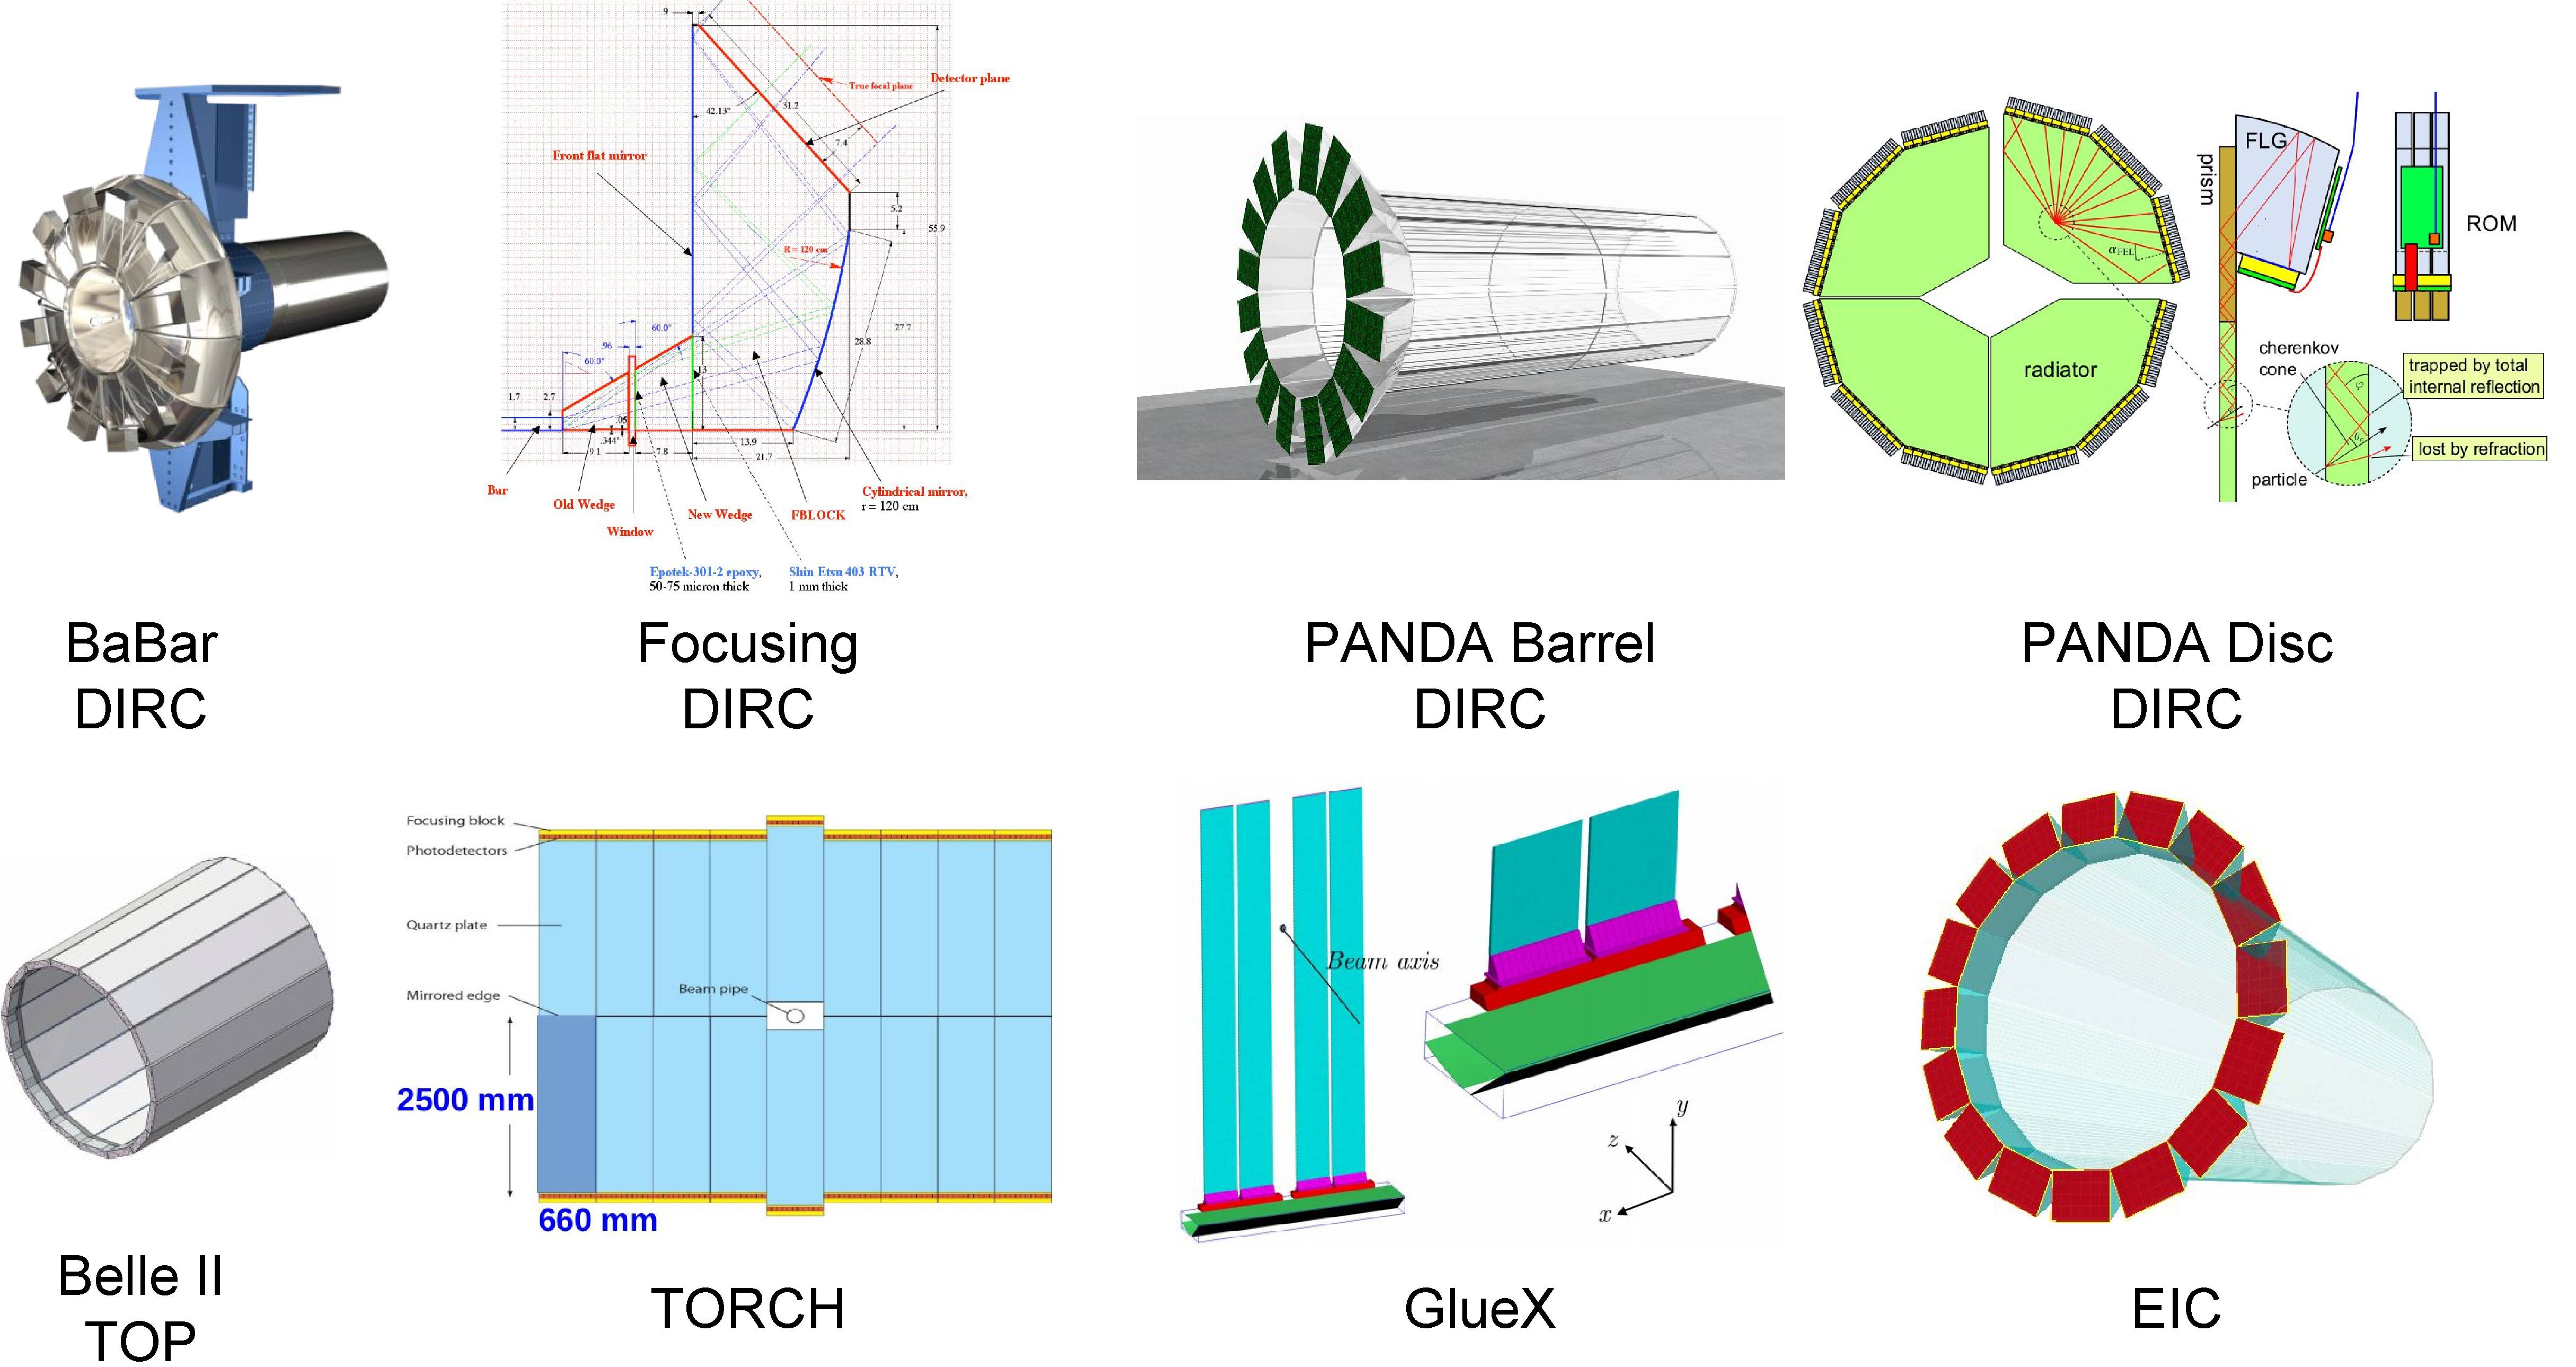
\includegraphics[width=\textwidth]{dirc_evolution.pdf}
	\caption{Evolution of the DIRC concept. From top left to bottom right: BaBar Barrel DIRC, Focusing DIRC, PANDA Barrel DIRC, PANDA Disc DIRC, Belle II Time of Propagation DIRC, LHCb TORCH DIRC, GlueX DIRC, EIC DIRC}
	\label{fig:dirc_evolution}
\end{figure}

%-------------------------------------------------------------------------------
%	RECONSTRUCTION SECTION
%-------------------------------------------------------------------------------
\section{Hit Patterns and Cherenkov Angle Reconstruction Methods}
As mentioned previously, a DIRC detector is a more compact RICH system that relies on internal reflection of the Cherenkov photons inside the radiating material. However, as is illustrated in Figure \ref{fig:dircbasics}, not all of the light produced inside the radiator is internally reflected as photons with an angle less than the critical angle (approximately 43 degrees for the interface from fused silica to air) with respect to the surface will escape the radiator. Because of this loss of photons the hit patter of a DIRC is only roughly half of a typical RICH ring. To complicate matters further, the image of this half ring is doubled depending on if the photon exiting the bar was last reflected from the top of the bottom of the radiator 
 % explination of DIRC technology
%
\chapter{High-Performance DIRC@EIC}
%----------------------------------------------------------------------
%	DIRC@EIC CHAPTER
%----------------------------------------------------------------------
\label{ch:eicdirc}
The BaBar DIRC was able to reach a performance of 3 standard deviations (s.d.) separation for pions and kaons at up to 4 GeV/c particle momentum. The PANDA Barrel DIRC wishes to achieve similar performance, but due to space constraints they will be using a smaller expansion volume and must therefore rely on optical focusing of the Cherenkov photons to reach this performance. In both cases the separation power requires a per track Cherenkov angle resolution (Eq. \ref{eq:performance}) of 2.5 mrad The physics goals of an EIC require a pion/kaon separation of 3 s.d. at up to 6 GeV/c momentum, which requires 1 mrad track Cherenkov angle resolution. The graph in Figure \ref{fig:PID_performance} shows pion-kaon separation as a function of particle momentum for different assumptions of the per track Cherenkov angle resolution, highlighting the achieved performance of BaBar and the desired performance of PANDA and EIC. In order to reach this high resolution in a compact space the EIC DIRC must incorporate cutting-edge technology in focusing optics and photo sensor granularity and timing resolution.

\begin{figure}[!htb]
	\centering
	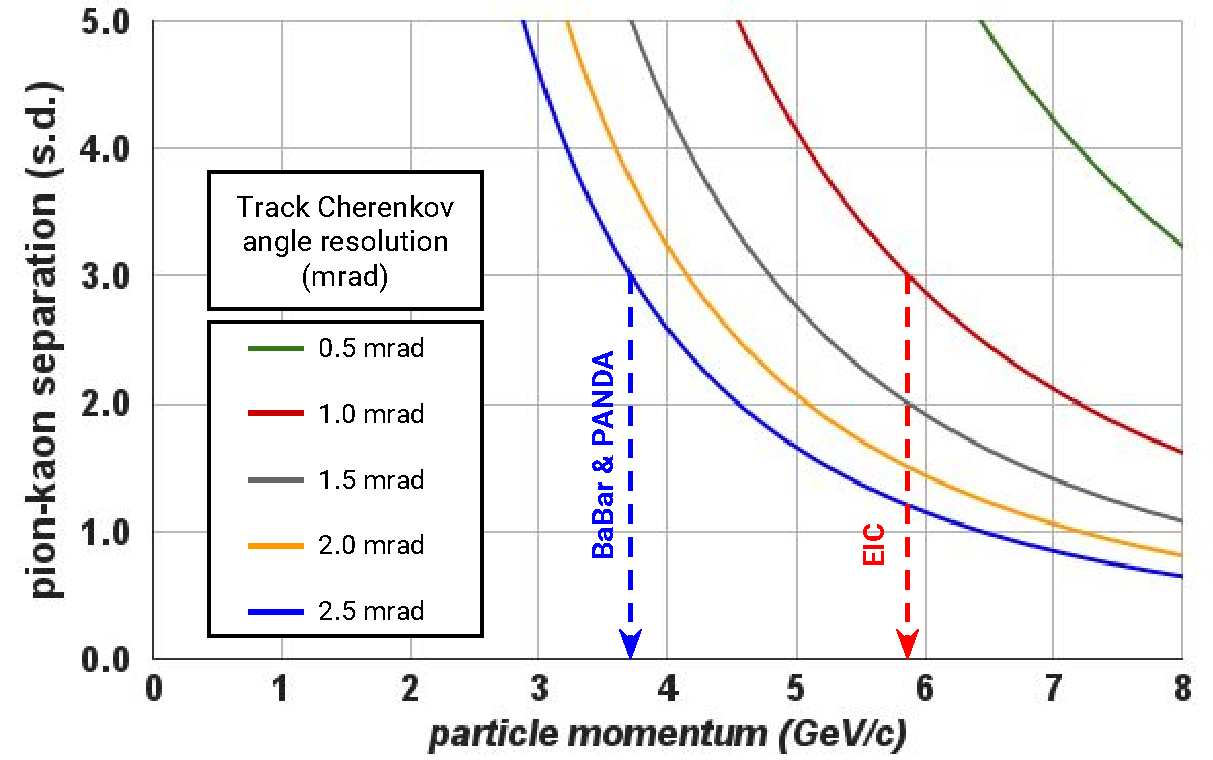
\includegraphics[width=\textwidth]{PID_performance.pdf}
	\caption{Pion-kaon separation as a function of particle momentum for different assumptions of the per track Cherenkov angle resolution. The PID requirements of the EIC necessitate a per track resolution of 1 mrad, while BaBar and PANDA needed only 2.5 mrad resolution.}
	\label{fig:PID_performance}
\end{figure}

%----------------------------------------------------------------------
%	CURRENT BASELINE DESIGN SECTION
%----------------------------------------------------------------------
\section{High-Performance DIRC Components and Design}
The baseline design of a DIRC for EIC has been constructed in a GEANT4 simulation based on that of the PANDA prototype DIRC, as shown in Figure \ref{fig:baseline_design}. There are 16 modules, called bar boxes, each containing 11 radiator bars 4200 mm long with a cross section of $17\times35.4\unit{mm}^2$. The 16 bar boxes are arranged in a barrel with a radius of 1 m around the beam line. Mirrors are coupled to one end of each bar, and a special 3-layer lens, discussed in more detail later, is attached to the other end. The lens is then coupled directly to a prism-shaped expansion volume made of fused silica, the same material as the radiator bars. The prism has an opening angle of $38^\circ$ with dimensions of $284.3\times390\times300\unit{mm}^3$. The $284.3\times390\unit{mm}^2$ detector plane of each prism is covered with micro-channel plate photomultiplier tubes (MCP-PMTs) with 27,690 $2\times2\unit{mm}^2$ pixels, for a total of 443,040 channels across the entire detector to record the location and arrival time of each detected Cherenkov photon. The dependence of the performance on the granularity of the detectors is shown later in this chapter.

\begin{figure}[!htb]
	\centering
	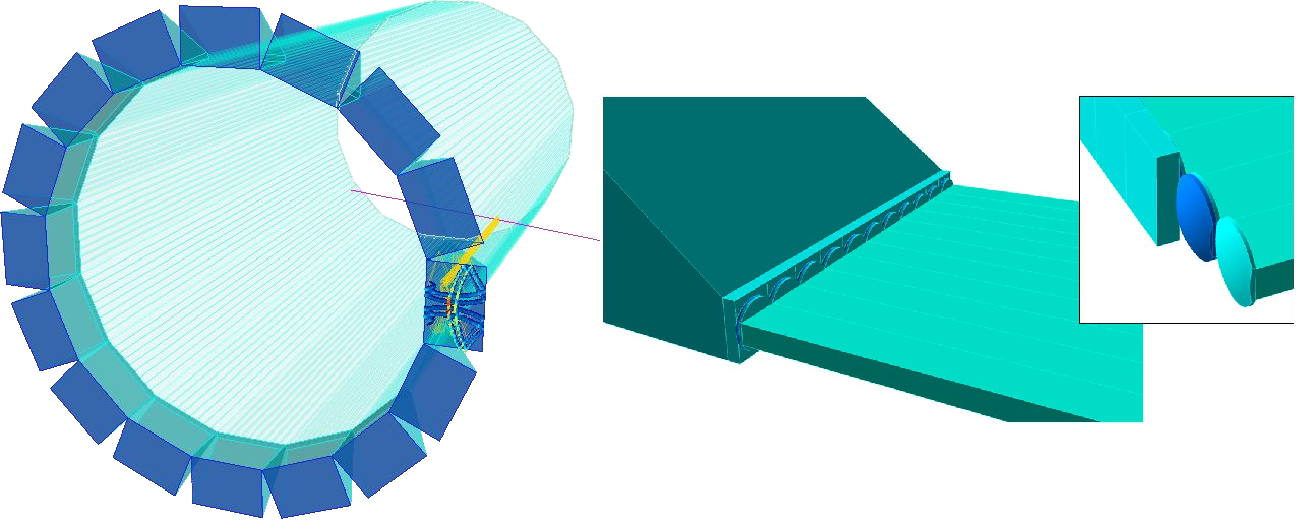
\includegraphics[width=\textwidth]{EIC_DIRC_baseline.pdf}
	\caption{Left: full GEANT4 simulation of the current DIRC at EIC baseline design with 16 bar boxes, 176 radiator bars, a 3-layer lens focusing optic, and a $38^\circ$ prism expansion volume. Right: a zoom in on a single bar box and the layering of the lens.}
	\label{fig:baseline_design}
\end{figure}

%----------------------------------------------------------------------
%----------------------------------------------------------------------
\subsection{Focusing Optics}

\begin{figure}[!htb]
	\centering
	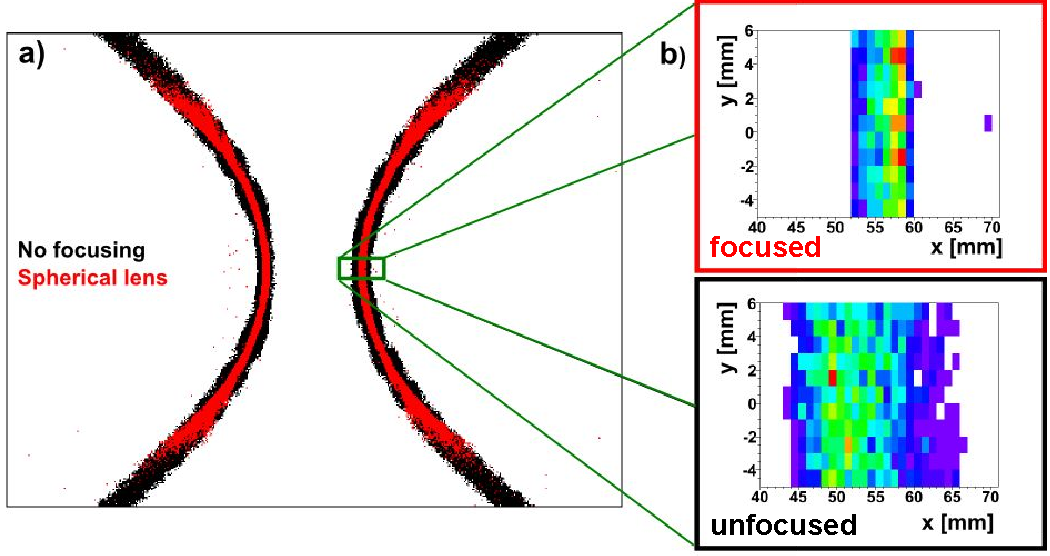
\includegraphics[width=\textwidth]{airgap_dispersion.pdf}
	\caption[Simulated hit pattern of PANDA DIRC without (black) and with (red) air gap lens focusing (a). On the outer edges of the ring image the lens is becoming dispersive  and losing photons, while near the center of the rings the lens does a good job of focusing the image, as seen more clearly in b).]{Simulated hit pattern of PANDA DIRC without (black) and with (red) air gap lens focusing (a) \cite{GregThesis}. On the outer edges of the ring image the lens is becoming dispersive  and losing photons, while near the center of the rings the lens does a good job of focusing the image, as seen more clearly in b).}
	\label{fig:airgap_dispersion}
\end{figure}

The pixel and bar size of a DIRC detector are important contributions to the Cherenkov angle resolution for small expansion volumes. The influence of the bar size can, however, be offset by focusing the Cherenkov photons. The FDIRC R\&D program first developed the concept of using focusing mirrors for DIRC detectors. The PANDA Barrel DIRC group settled on using a focusing lens between the radiator bar and the expansion volume. A standard lens made of fused silica with an air gap between the lens and the expansion volume was first studied. However, the focal plane of a single lens is highly parabolic in shape. Figure \ref{fig:airgap_dispersion} shows that while an air gap lens provides good focusing of the Cherenkov pattern in the central region of the ring, where photons are more or less perpendicular to the lens, it becomes defocused nearer to the edges of the pattern and loses photons. This deterioration of the image quality for steeper angles is a combination of lens aberrations, the curved focal plane, and the so-called kaleidoscopic effect \cite{FDIRCMathematica}.

A 2-layer compound lens composed of fused silica and a layer of high-refractive index material Lanthanum crown glass (NLaK33) \cite{SchottData}, $n \approx 1.75$, was also studied. This design couples directly to the expansion volume, greatly reducing the loss of photons at steeper angles. Figure \ref{fig:lens_photon_yield} shows a comparison of the photon yield from a bar radiator with no focusing (green), a standard air gap lens (red), and a 2-layer lens (blue) for two cases. In the $125^\circ$ case (left) both lenses have comparable photon yields, because the angle between the photons and the lens is fairly shallow. In the $90^\circ$ case (right), however, the photon yield for the air gap lens is dramatically lowered due to the steep angles between the photons and the lens. The photon yield for the no focusing option is quite deceiving in that it produces a much higher average photon yield than either lens, but the reconstruction of the Cherenkov angle is nearly impossible to within a reasonable measure for the perpendicular case.

\begin{figure}[!htb]
	\centering
	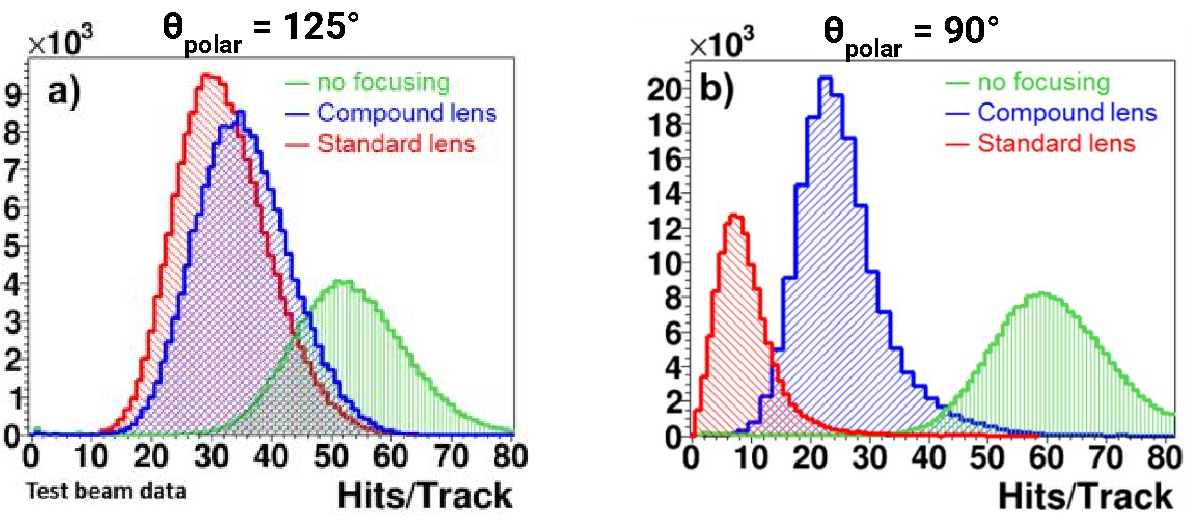
\includegraphics[width=\textwidth]{lens_photon_yield_comparison.pdf}
	\caption[Comparison of the photon yield per track for a DIRC bar with no focusing (green), a standard air gap lens (red), and a 2-layer compound lens (blue) for polar angles of $125^\circ$ (left) and $90^\circ$ (right) \cite{GregThesis}. The standard and compound lenses have comparable yields at $125^\circ$, but the standard lens clearly loses a large amount of photons in the perpendicular case.]{Comparison of the photon yield per track for a DIRC bar with no focusing (green), a standard air gap lens (red), and a 2-layer compound lens (blue) for polar angles of $125^\circ$ (left) and $90^\circ$ (right). The standard and compound lenses have comparable yields at $125^\circ$, but the standard lens clearly loses a large amount of photons in the perpendicular case.}
	\label{fig:lens_photon_yield}
\end{figure}

The 2-layer lens design solves the problem of photon yield loss from the air gap lens at steeper angles and will allow the PANDA Barrel DIRC to reach their desired separation power. However, as discussed earlier, this separation power of 3 s.d. at 4 GeV/c is insufficient for the requirements of a DIRC at EIC. The key to solving this problem was in designing a special 3-layer spherical compound lens. The advantage of this 3-layer lens design over a traditional optical lens or the 2-layer lens is the shape of the focal plane. According to simulation the focal plane of the 3-layer lens is relatively flat, as shown in Figure \ref{fig:lens_focal_plane}. Photos of a prototype lens tested at CERN in 2015 and an exploded view of the lens layers and dimensions are shown in Figure \ref{fig:3CS_schematic}. It contains a layer of NLaK33 sandwiched between two layers of fused silica. The two radii of the middle layer were optimized to remove aberrations present in standard lenses by first defocusing and then refocusing transmitted photons to create a flat focal plane, matching the geometry of the prism expansion volume. Five prototype lenses were produced for evaluating the performance of the lens design in a test beam, for measuring the radiation hardness of the NLaK33 material, and for evaluating the focal plane. These tests will be discussed in greater detail in Chapters \ref{ch:components} and \ref{ch:analysis}.

\begin{figure}[!htb]
	\centering
	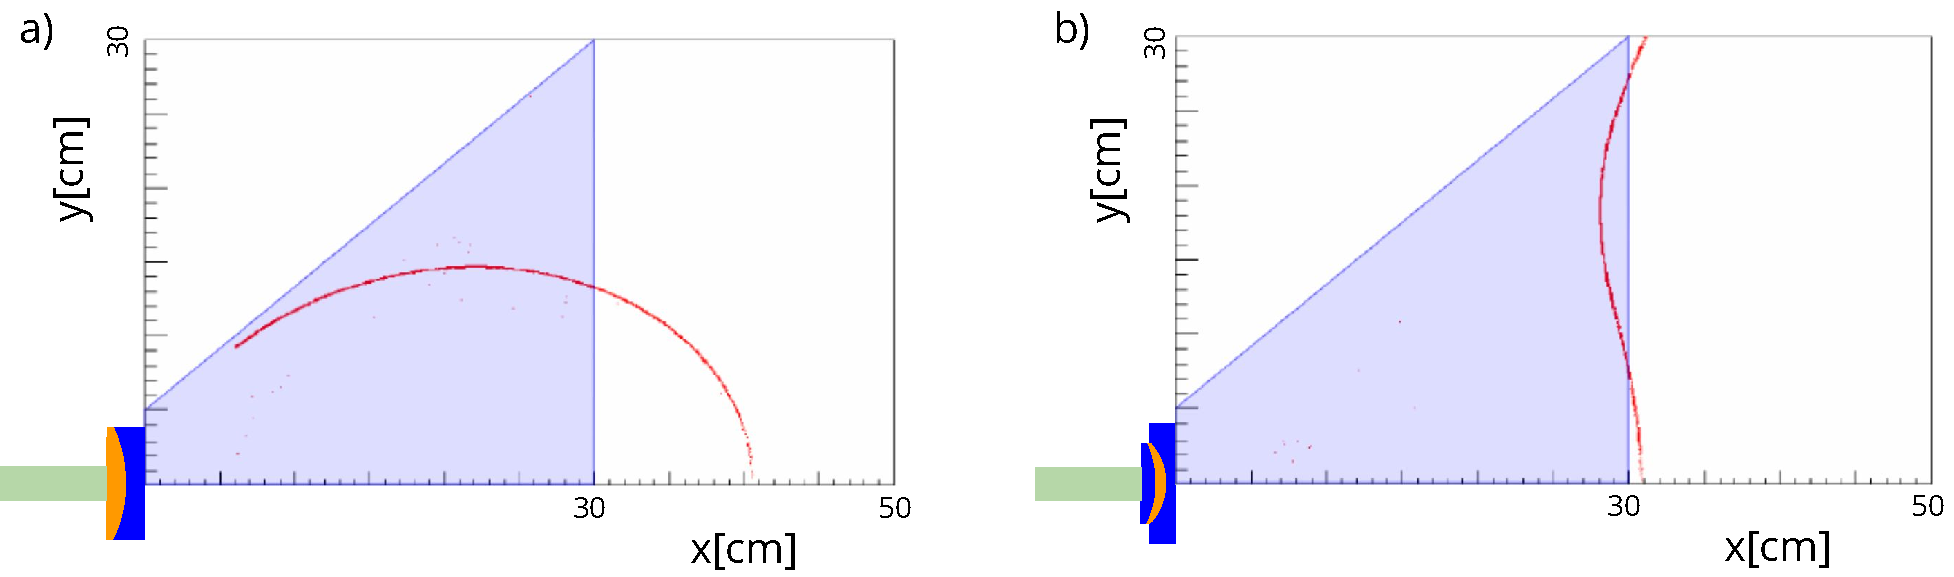
\includegraphics[width=\textwidth]{lens_comparison}
	\caption{The simulated focal planes (red lines) of a 2-layer lens (left) and the 3-layer lens (right) compared to the shape of the expansion volume prism (grey). Obviously the focal plane of the 2-layer lens is highly parabolic in shape, whereas the 3-layer lens focal plane is relatively flat, allowing for a better resolution of the Cherenkov angle.}
	\label{fig:lens_focal_plane}
\end{figure}

\begin{figure}[!htb]
	\centering
	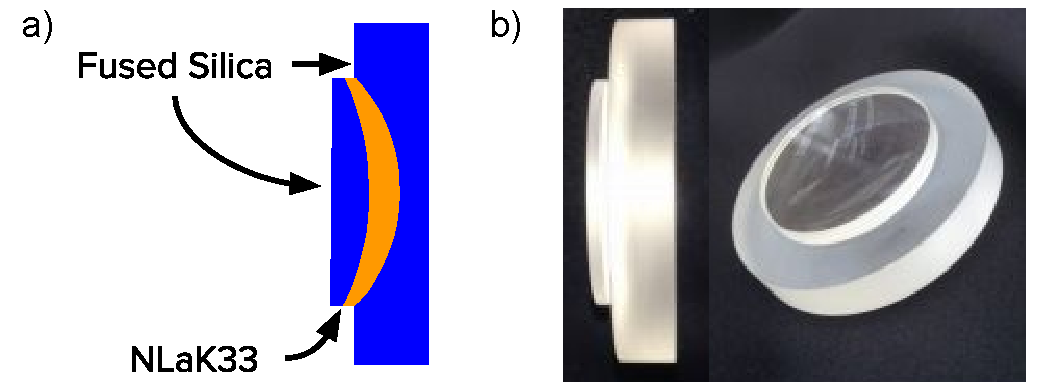
\includegraphics[scale=0.7]{3CS_schematic.pdf}
	\caption{Prototype 3-layer lens built for optical testing (a), and an exploded view of each layer with dimensions (b).}
	\label{fig:3CS_schematic}
\end{figure}

%----------------------------------------------------------------------
%----------------------------------------------------------------------
%\subsection{Sensors}

%----------------------------------------------------------------------
%	SIMULATION SECTION
%----------------------------------------------------------------------
\clearpage
\section{Simulated Performance}

\subsection{Geometric Reconstruction}
Simulated reconstructions of the Cherenkov angle for kaons and pions at 6 GeV/c with a $125^{\circ}$ polar angle using the design parameters above are shown in Figure \ref{fig:EIC_reconstruction}. The signal is very clean and the mean and SPR of the distribution are easily extracted. Figure \ref{fig:EIC_performance}a shows the photon yield, or multiplicity, per polar angle for fifty 6 GeV/c pions, and Figure \ref{fig:EIC_performance}b shows the Single Photon Resolution (SPR) \footnote{Three points are normally required to define a circle and thus extract a radius. However, with a perfect RICH detector it is sufficient to know only a single point on the ring as one also knows the center of the circle (i.e. the particle track). Here, too, it is sensible to talk about the resolution of single photon events as the center of the ``circle" for a DIRC (i.e. the polar angle) is known from tracking.} per polar angle for fifty 6 GeV/c kaons (red) and pions (blue). The per track Cherenkov angle resolution, given by Eq. (\ref{eq:performance}), is shown in Figure \ref{fig:EIC_track_res} for assumptions of 0.25 mrad (black), 0.5 mrad (red), 0.75 (green), and 1 mrad (blue) correlated term contributions with 6 GeV/c pions \footnote{NB: the per track Cherenkov angle resolution will be slightly different for each particle species, however, because the SPR for each particle is almost identical, showing only the results for pions is sufficient.}.  The simulations were done assuming that the sides of the 3-layer lens focusing optic were not reflective, therefore reducing the photon yield and making the performance slightly worse.

The SPR of the reconstructed Cherenkov angle was found to scale with the pixel size of the MCP-PMTs roughly as $SPR \approx SPR_{0}\sqrt{1+size^2/a^2}$, as shown in Figure \ref{fig:EIC_sensor_scaling}. Clearly the 4 mm pixel size, though not ideal, is comparable in performance to the 2 mm pixel size. This is an important factor to consider in the final design due to the increase of the cost per pixel of MCP-PMTs and with the electronics readout per channel as the size of the pixels decreases.


\begin{figure}[!htb]
	\centering
	\includegraphics[width=\textwidth]{{EIC_theta_K+_125.00}.png}
	\includegraphics[width=\textwidth]{{EIC_theta_pi+_125.00}.png}
	\caption{Reconstructed $\thetaC$ spectrum for 6 GeV/c kaons (top) and pions (bottom) and a $125^{\circ}$ polar angle.}
	\label{fig:EIC_reconstruction}
\end{figure}

\begin{figure}[!htb]
	\centering
	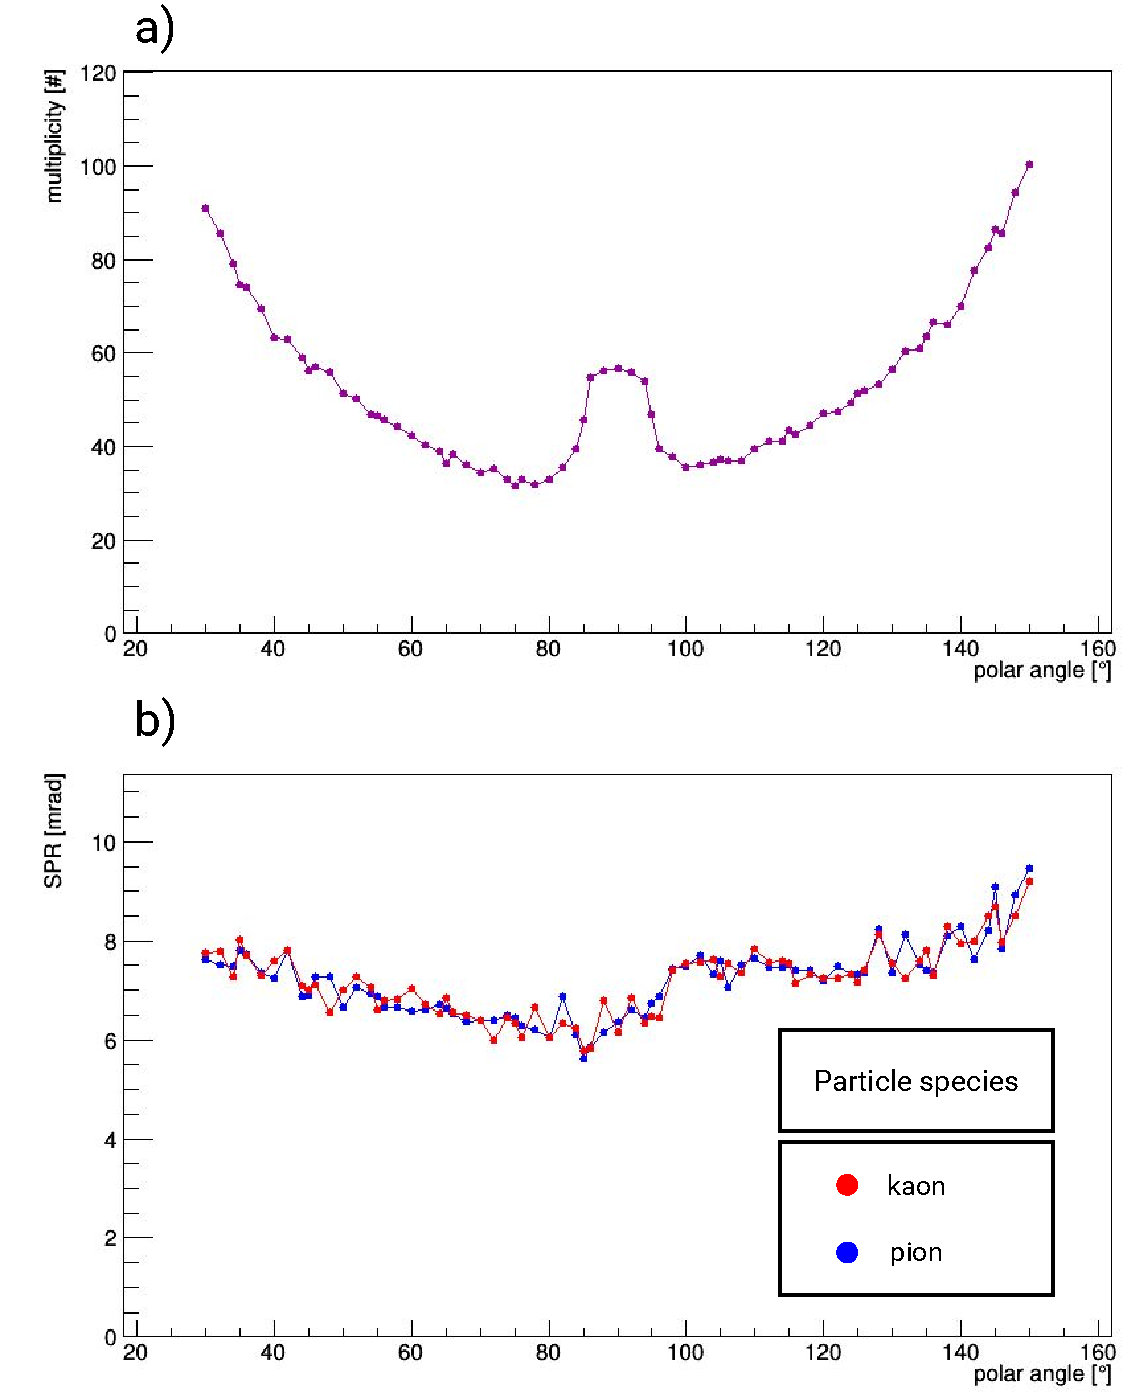
\includegraphics[width=\textwidth]{EIC_performance.pdf}
	\caption{The multiplicity (a) and SPR (b) performance per polar angle of the EIC DIRC baseline design. Plots were generated using fifty particles (kaons in red, pions in blue) at 6 GeV/c per polar angle.}
	\label{fig:EIC_performance}
\end{figure}

\begin{figure}[!htb]
	\centering
	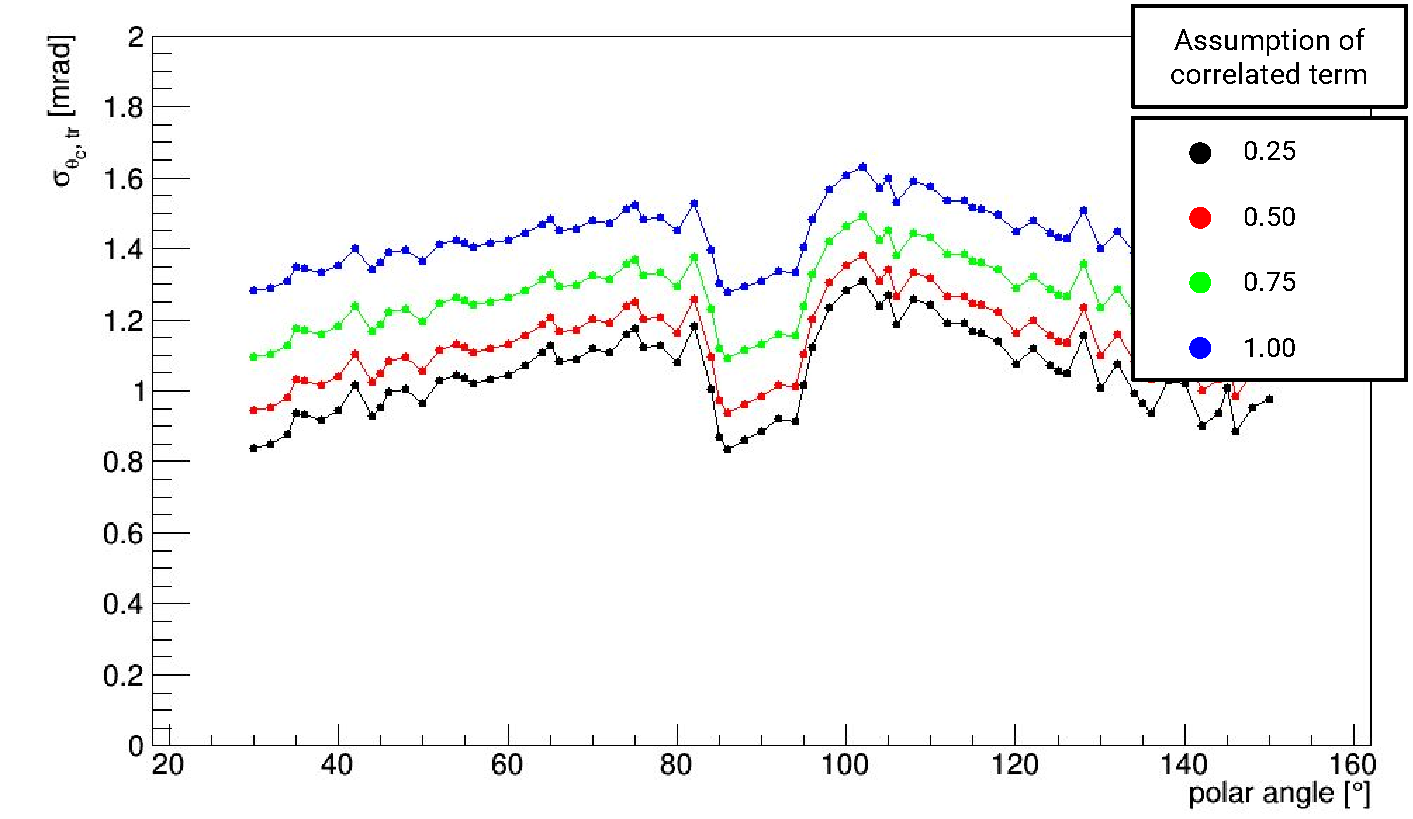
\includegraphics[width=\textwidth]{EIC_track_res.pdf}
	\caption{The per track Cherenkov angle resolution of the EIC DIRC with different assumptions of the correlated term, $\sigma_{correlated}$: 0.25 mrad (black), 0.5 mrad (red), 0.75 (green), and 1 mrad (blue).}
	\label{fig:EIC_track_res}
\end{figure}

\begin{figure}[!htb]
	\centering
	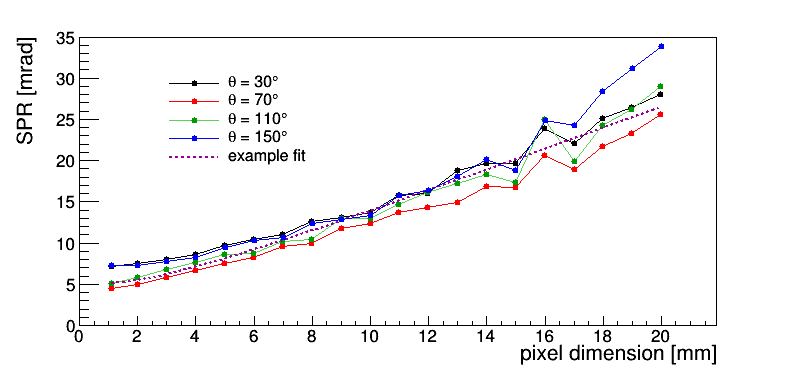
\includegraphics[width=\textwidth]{EIC_SPR_vs_sensorDim3.png}
	\caption{Scaling of the SPR as a function of the MCP-PMT pixel dimension for $30^\circ$ (black), $70^\circ$ (red), $110^\circ$ (green), and $150^\circ$ (blue) polar angle along with an example fit (dashed purple) showing that the dependence of the performance scales roughly as $\sqrt{1+\frac{pixel^2}{a^2}}$}
	\label{fig:EIC_sensor_scaling}
\end{figure}

\subsection{Time-based Reconstruction}
The methods for time-based reconstruction, as described in Chapter \ref{ch:dirc}, were also implemented for the EIC DIRC: 60,000 pions and kaons were simulated in GEANT4 using the current EIC DIRC design geometry and PDFs were generated for each detector pixel; the PDFs were then used to produce log-likelihood separation for each particle hypothesis. Figure \ref{fig:EIC_timebased_ex} shows the log-likelihood separation for pions and kaons at polar angle of $30^\circ$.  Figure \ref{fig:EIC_timebased_performance} shows the separation power (top) and the PID efficiency/mis-identification over all polar angles.

\begin{figure}[!htb]
	\centering
	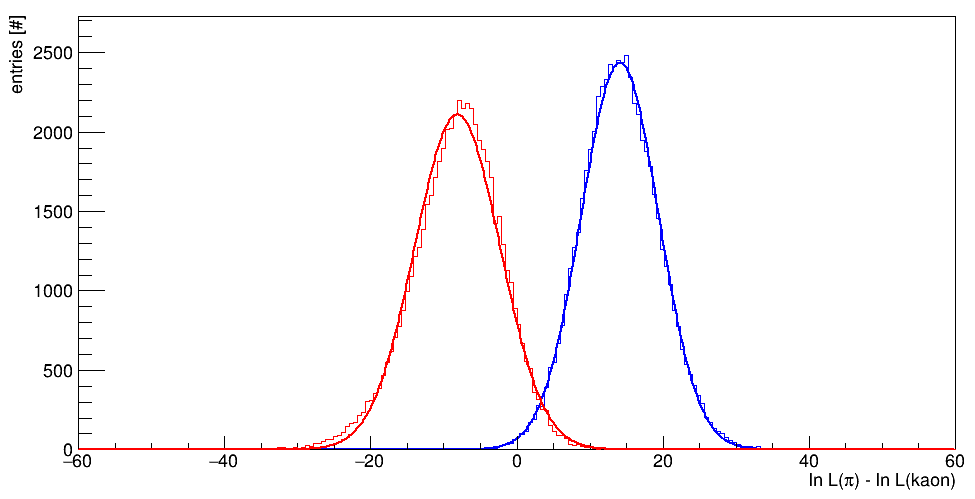
\includegraphics[width=\textwidth]{EIC_30deg_timebased_sep.png}
	\caption{Example of log-likelihood separation for pions (red) and kaons (blue) at $30^\circ$ polar angle using time-based reconstruction.}
	\label{fig:EIC_timebased_ex}
\end{figure}

\begin{figure}[!htb]
	\centering
	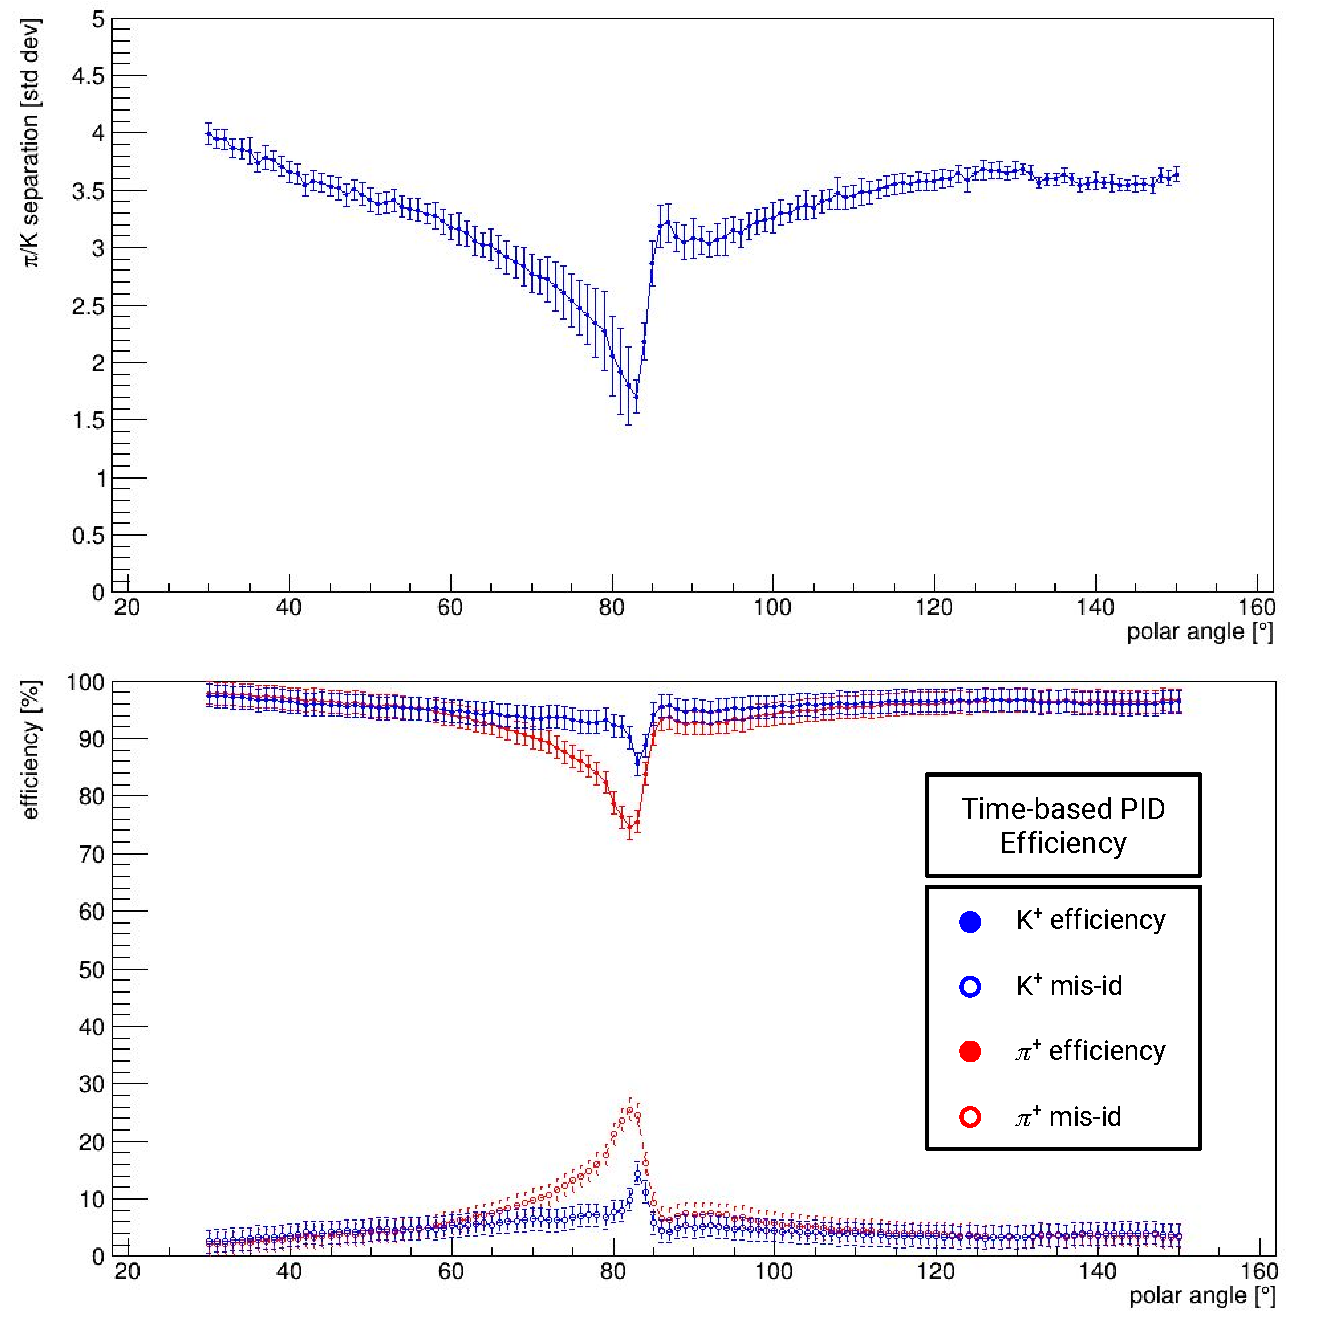
\includegraphics[width=\textwidth]{EIC_timebased_performance.pdf}
	\caption{\textbf{Top}: Separation power as a function of polar angle for 6 GeV/c pions and kaons using time-based reconstruction. \textbf{Bottom}: Efficiency (solid circles) of PID as a function of polar angle for pions (red) and kaons (blue) along with the mis-identification rate (open circles).}
	\label{fig:EIC_timebased_performance}
\end{figure}

Overall the results for both geometric and time-based reconstruction show that due to the design's large expansion volume, small pixel size, and ease of signal reconstruction the performance of this design can reach the desired performance for the required physics.
%----------------------------------------------------------------------
%	DESIGN OPTIMIZATIONS SECTION
%----------------------------------------------------------------------
%\section{Potential Optimizations}
 % specifications of high-performance DIRC@EIC
%
%\chapter{Test Bench Evaluation of DIRC@EIC Components}
\chapter{Testing DIRC Components}
%----------------------------------------------------------------------
%	DIRC TECHNOLOGY CHAPTER
%----------------------------------------------------------------------
\label{ch:components}
The validation of the key components of the DIRC for an EIC discussed in Chapter \ref{ch:eicdirc} is vital to show that the GEANT4 simulation package produces results expected for the real detector. However, due to budget restraints it was not possible to build or otherwise procure a full scale prototype of the envisioned EIC DIRC discussed in Chapter \ref{ch:eicdirc}. As a conservative estimate of the cost of a simple prototype: one radiator bar is \$20k, a prism expansion volume is \$30k, a 3-layer lens is \$10k, and an array of 24 (4x6) sensors is \$200k. On top of this, the cost of a test beam run would be roughly \$10k for travel and expenses.  This roughly \$300k expense for one prototype and test beam is highly impractical given that the budget for all detector work for the EIC R\&D effort (RICH, Time-of-Flight, simulation studies, calorimetry, etc) is only \$1M/year\footnote{It should be noted that once the Department of Energy approves the construction of an EIC, but before breaking ground on the facility, the budget for R\&D will be expanded such that building a baseline-design EIC DIRC prototype will be viable}. Instead a series of test bench measurements have been made to validate simulated performance of the new 3-layer lens design, study the radiation hardness of the NLaK33 material, and evaluate the performance of MCP-PMTs in high magnetic field environments. A synergistic test beam effort with the PANDA Barrel DIRC group was also performed at CERN in 2015, but will be discussed in greater detail in Chapter \ref{ch:analysis}.

%----------------------------------------------------------------------
%	3-LAYER LENS OPTICS SECTION
%----------------------------------------------------------------------
\section{Optical Properties of 3-Layer Lens}
\begin{figure}[!htb]
	\centering
	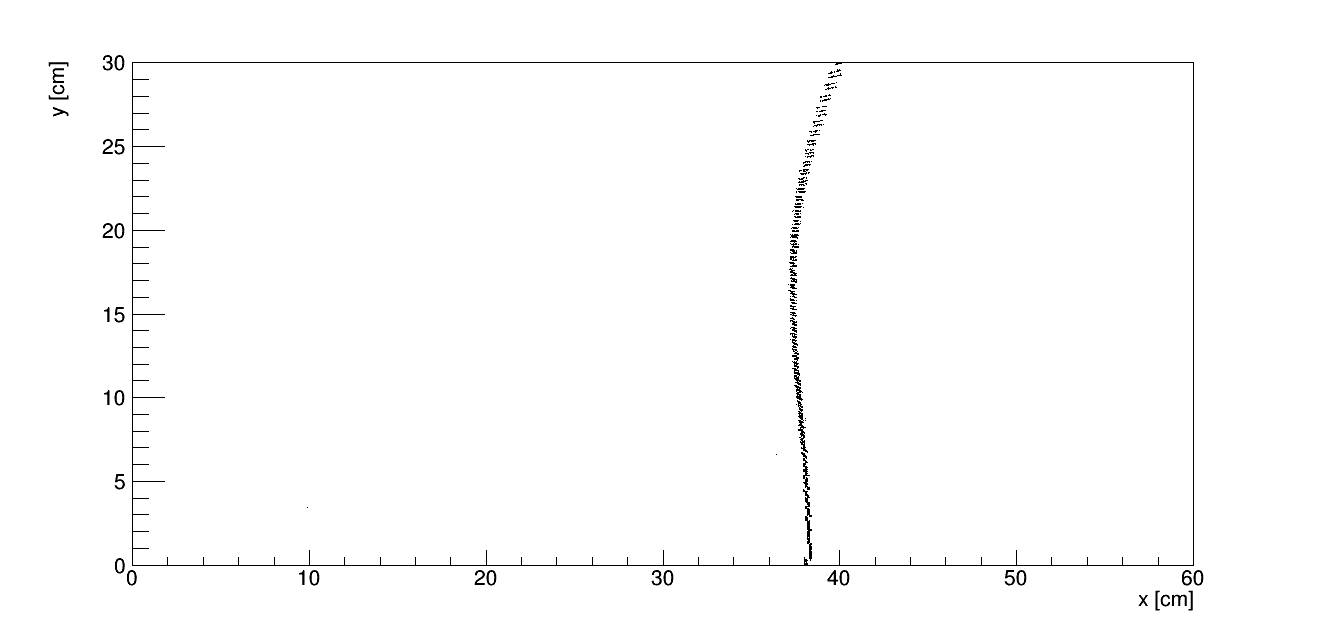
\includegraphics[width=\textwidth]{2D_plane.png}
	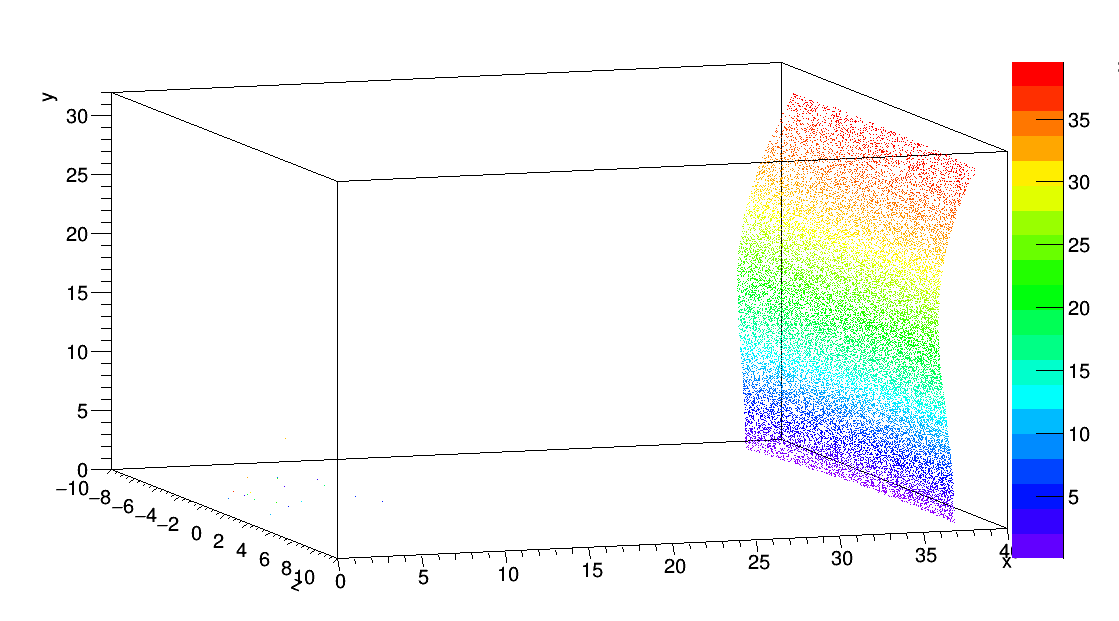
\includegraphics[width=\textwidth]{3D_plane_angle.png}
	\caption{Simulation of the 3-layer lens focal plane with all photons confined to a single plane (top) and the full 3D focal plane (bottom). The color scale corresponds to the initial angle (in degrees) between the laser beams and the lens face. The 3D plane has been constrained to the y/z dimensions of the current expansion volume for the EIC DIRC. The ``beams" of photons in the simulation were centered around the center of the lens with a separation of 2 mm.}
	\label{fig:focalplane_sim}
\end{figure}
\begin{figure}[!htb]
	\centering
	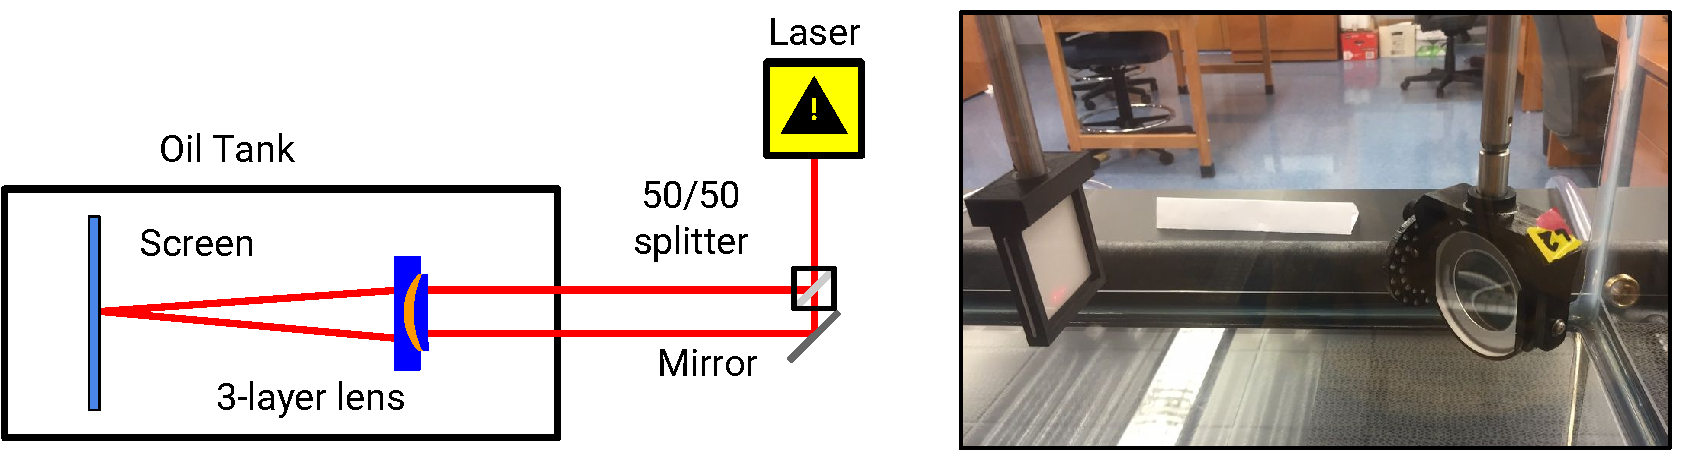
\includegraphics[width=\textwidth]{lens_setup_schematic.pdf}
	\caption{Schematic drawing of the setup built at Old Dominion University for testing the optical properties of the 3-layer lens design (left), and a closeup view of the lens and screen inside the actual setup (right).}
	\label{fig:ODU_setup}
\end{figure}

\begin{figure}[!htb]
	\centering
	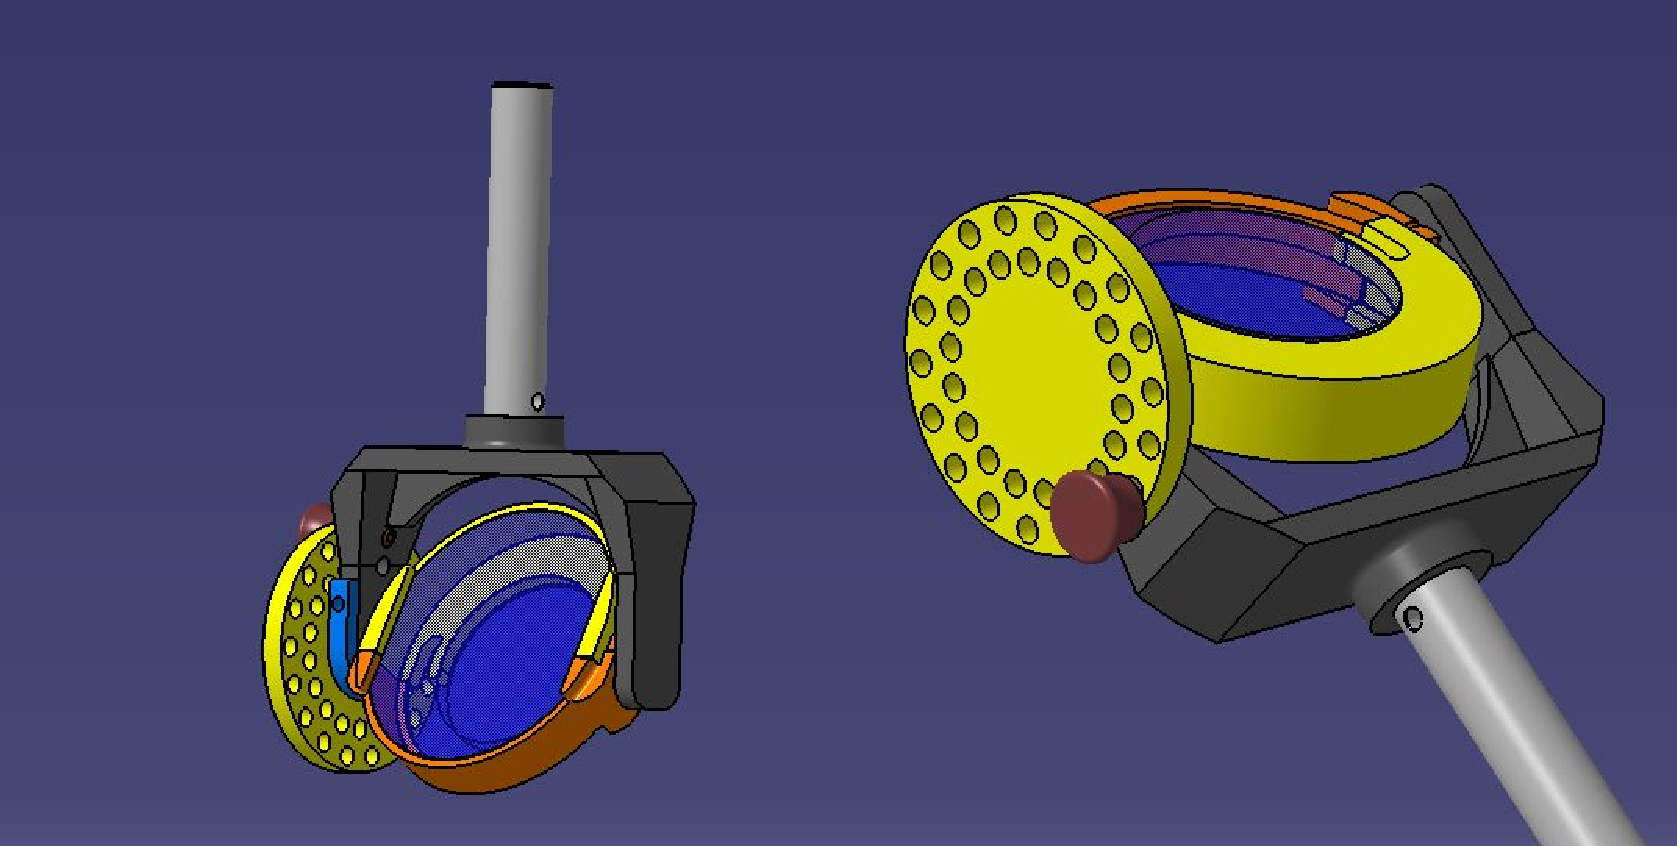
\includegraphics[width=\textwidth]{lens_holder.pdf}
	\caption{CAD drawing of 3-layer lens holder which allows precision rotation in two orthogonal, allowing the full 3D focal plane to be mapped.}
	\label{fig:lens_holder}
\end{figure}

\begin{figure}[!htb]
	\centering
	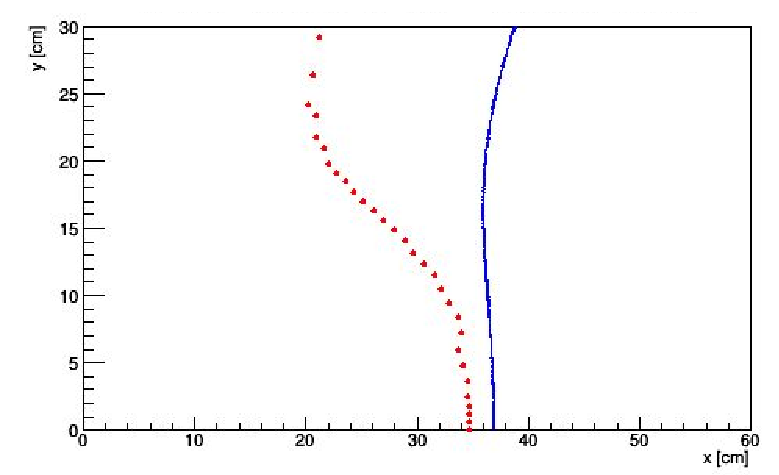
\includegraphics[width=\textwidth]{focalplane_initial.pdf}
	\caption{Initial measurement of the 3-layer lens focal plane using the upgraded green laser (red dots) compared to simulation (blue line). Note that this figure is for illustrative purposes only. The measurement techniques used to measure the focal plane were changed to match the simulation, shown in Figure \ref{fig:focalplane_corrections}.}
	\label{fig:focalplane_initial}
\end{figure}

\begin{figure}[!htb]
	\centering
	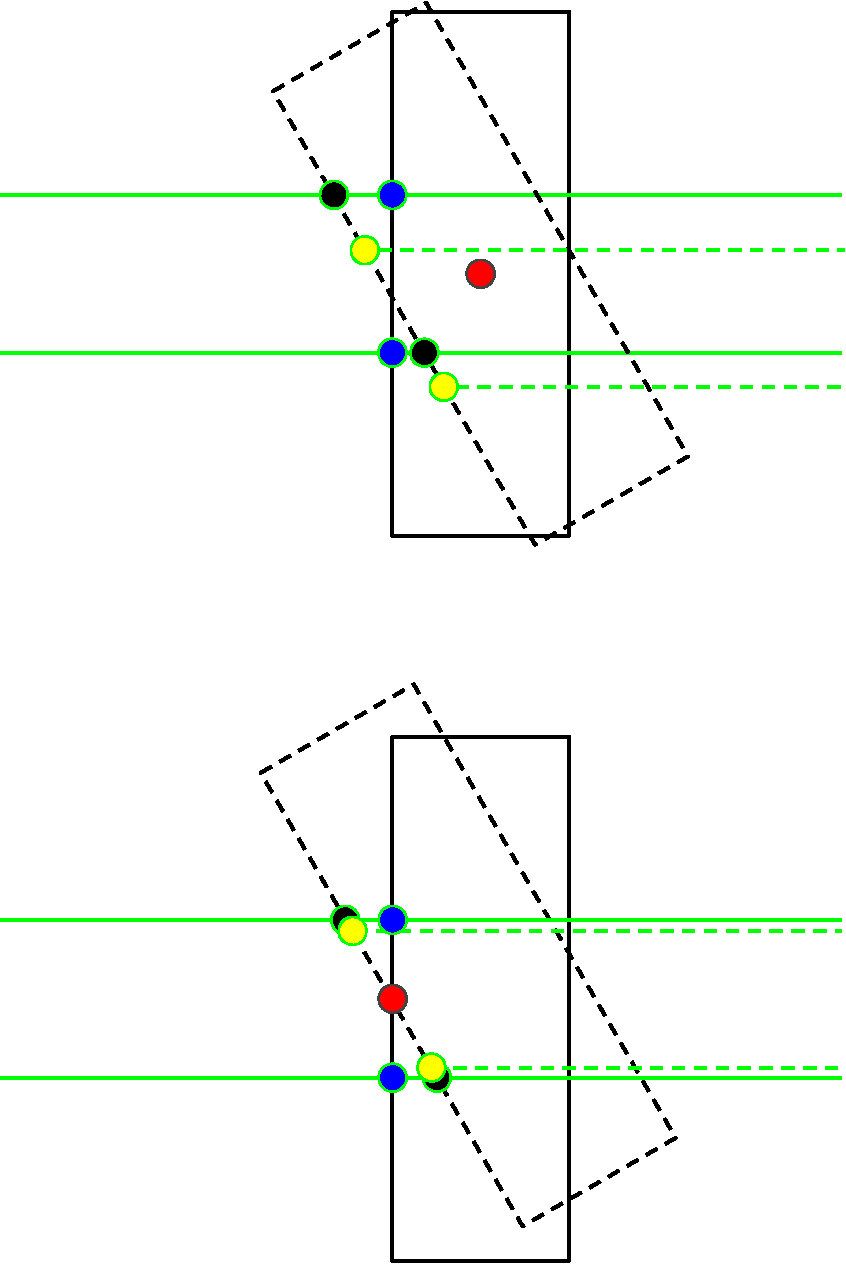
\includegraphics[width=0.43\textwidth]{lens_rotation_point.pdf}
	\caption{Illustration of the discrepancy between beam positions in data (black) and simulation (yellow) in relation to the original beam positions (blue) for a given rotation point (red) at the center (top) of the lens, or at the edge (bottom) of the lens. }
	\label{fig:lens_rotation_point}
\end{figure}

\begin{figure}[!htb]
	\centering
	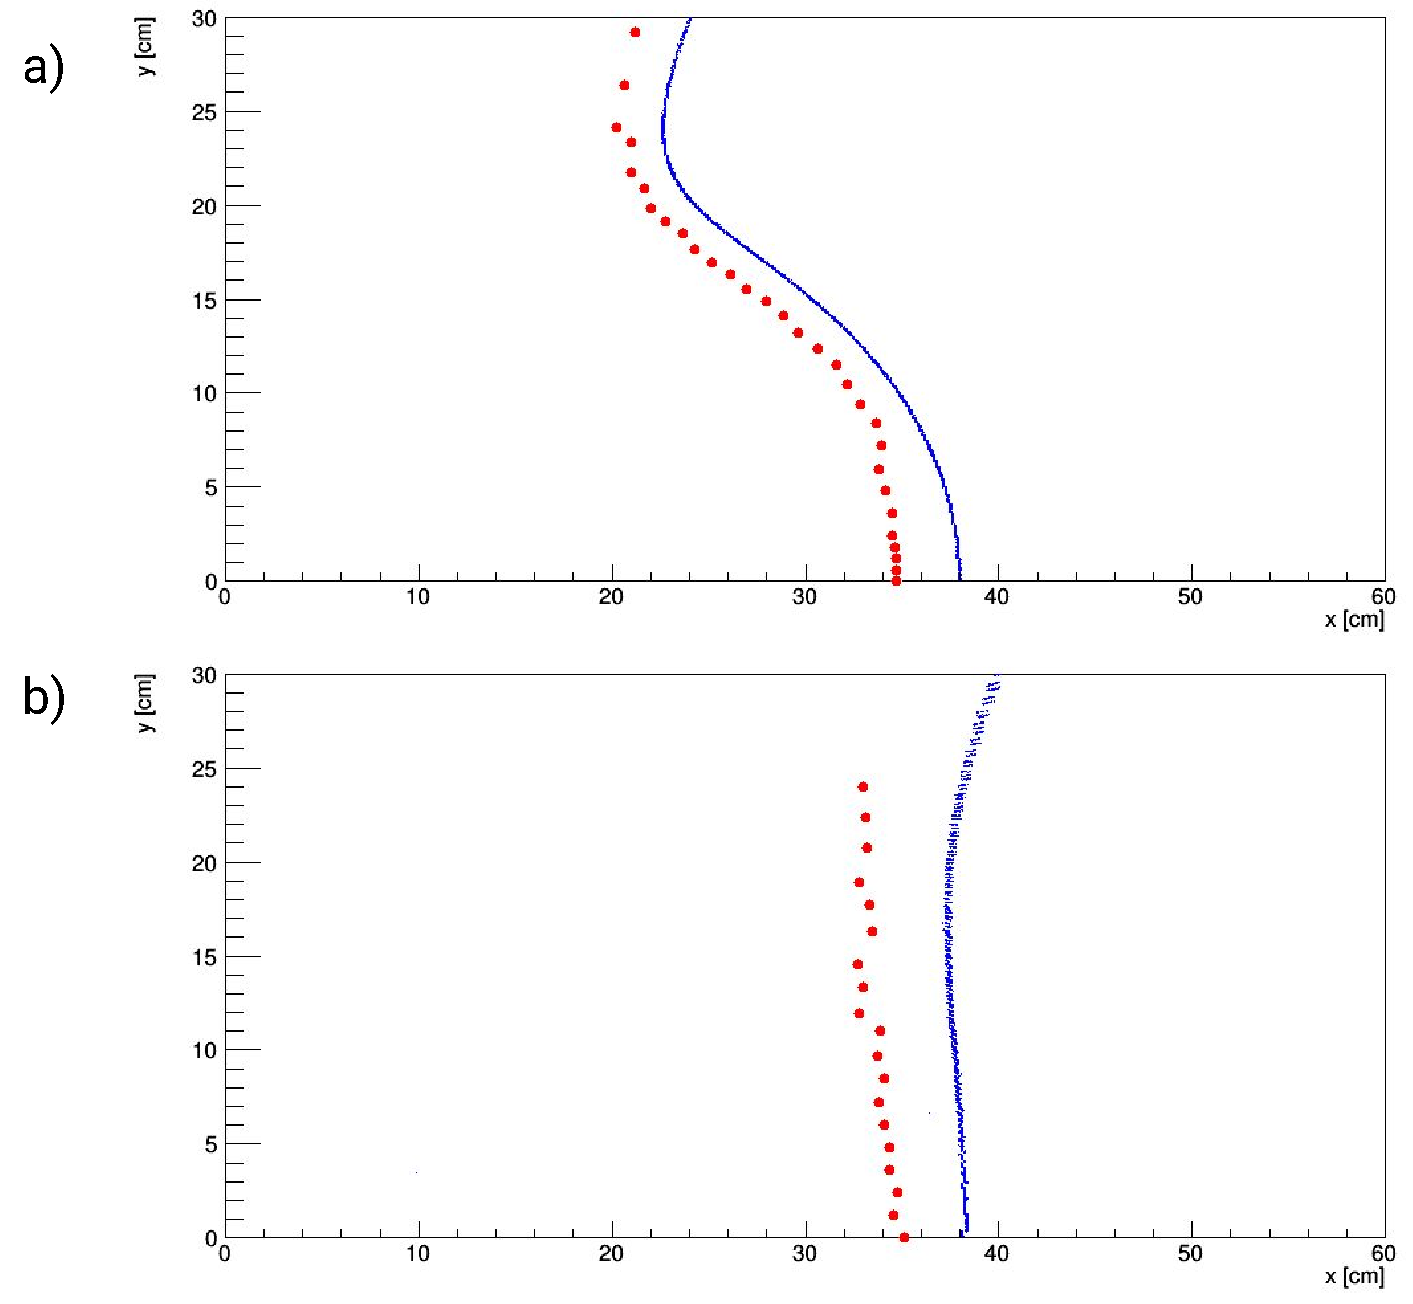
\includegraphics[width=\textwidth]{focalplane_corrections.pdf}
	\caption{Initial measurement of the 3-layer lens focal plane compared to a rotation corrected simulation (a), and a second measurement with a tighter (2 mm) beam configuration and a modified lens holder (b).}
	\label{fig:focalplane_corrections}
\end{figure}

The purpose of the 3-layer lens design is to provide a mostly flat, uniform focal plane to follow the face of the detector plane. Doing so provides better resolution and hence better performance compared to standard focusing options, which typically have very curved, hyperbolic focal planes. A GEANT4 simulation of the nominal (top) and full 3D focal plane (bottom) of the lens are shown in Figure \ref{fig:focalplane_sim}. The 3D plane has been limited to the size of the detector plane anticipated for the EIC DIRC, and the color scale indicates the angle at which photons intersected the front face of the lens. Because only the total focal length is of interest the depth of the expansion volume was limited so that no bounces occurred.

To measure the shape of the focal plane a setup was designed and built, shown in Figure \ref{fig:ODU_setup}, at Old Dominion University in which a laser shines through a 50/50 beam splitter and a mirror to make two parallel beams. Initially the beams were separated by 5 mm, but gradually the distance was reduced to 1 mm in order to attempt to avoid non-uniform aberrations due to small misalignments as much as possible. The beams then pass through a $30\times40\times60\unit{cm}^3$ glass container filled with Britol 9NF White Mineral Oil \cite{BritolOil} with a refractive index similar to that of fused silica to simulate the behavior of light passing from bar to lens to expansion volume. The beams are focused through the 3-layer lens prototype, being held in a specially designed holder that allows the lens to be rotated in two planes (Figure \ref{fig:lens_holder}). Finally the beams are focused onto a plastic screen inside the tank that is attached to a track and allowed to slide freely. Due to the relatively low resolution of the human eye and the finite size of the beams the exact point of focus was difficult to measure, so an averaging method was used in which the median of the two points where the beams seem to converge and diverge was taken to be the focal point (see Figure \ref{fig:laser_crossing}). This lead to much more accurate and reproducible results.

\begin{figure}[!htb]
	\centering
	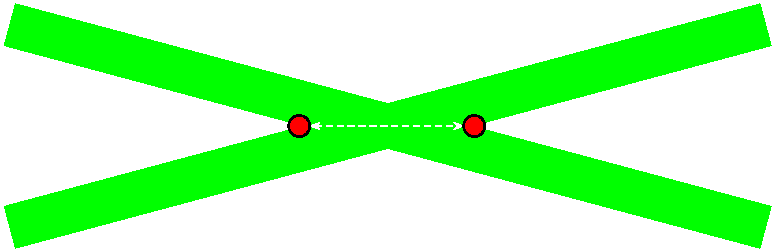
\includegraphics[width=\textwidth]{laser_crossing.pdf}
	\caption{Illustration of two crossing laser beams (green) with finite size. During measurements all the space between the two red circles was perceived as a single point. To counteract this effect the focal point was taken as the average point between where the beams first seem to come together and where they seem to again separate.}
	\label{fig:laser_crossing}
\end{figure}

Measurements were initially taken with a 632 nm red helium-neon laser, but the beam spot was too large and very distorted. A 530 nm wavelength green laser with a 1 mm beam spot was then purchased as a replacement. Initial results with a 5 mm beam separation are shown in Figure \ref{fig:focalplane_initial}. Obviously there is a large discrepancy in both position and shape of the measured and simulated focal plane. This was rectified by discovering that in the simulation it was assumed that the two beams were entering the lens at fixed points on the lens' face regardless of lens rotation, where as in the experiment the rotation of the lens about it's center causes the beams to shift with respect to the lens face. When rotating at the edge of the lens closest to the laser rather than through the center this difference is negligible, as illustrated in Figure \ref{fig:lens_rotation_point}.

A correction was implemented in the GEANT4 simulation to account for the shift of the beam spot during rotation, the results of which can be seen in Figure \ref{fig:focalplane_corrections}a. The beams have since been brought to a 2 mm separation to reduce effects of aberration and a second lens holder was 3D printed to allow for rotation about the edge of the lens. A new round of data was taken and results are shown in Figure \ref{fig:focalplane_corrections}b. This change vastly improved the results of both the simulation from the first measurement and the results of the second, showing that the simulation indeed reproduces very nicely the shape of the focal plane, although the position is still roughly 3 cm too long.

The absolute position of the focal plane can be explained in several ways: the second curved surface of the 3-layer lens has a slightly smaller radius than was requested, the NLaK33 material has a slightly larger index of refraction than anticipated, the NLaK33 layer is slightly thicker than was requested, the laser beams in the experimental setup are not parallel, the index of refraction of the mineral oil is not equivalent to that of fused silica, or some small contribution from any and all of these effects. Unfortunately, measuring these quantities is currently not achievable. However, the GEANT4 simulation can manipulate them with high precision to study their effects on the focal plane.

Figure \ref{fig:focal_plane_shifts} shows by how much each of these parameters must be adjusted such that the point with $0^\circ$ rotation and tilt angles agrees with the same point measured in the lab, along with the ``perfect" simulation, which assumes all default parameters are correct, for comparison. A decrease in the index of refraction of the mineral oil of $0.15$ (pink) is unrealistic due to the drastic change in the focal plane. Likewise, an increase in the index of refraction of the lanthanum crown glass by $0.03$ (green) is not realistic due to the large difference between needed value for the simulation and the specifications sheet. A decrease in the radius of the second layer of the lens by $1.3$~mm (blue), and a convergent angle of $0.15$~mrad between the beams (black) do, however, seem reasonable in describing this systematic shift of the focal plane. 

As it is impossible to measure the curvature of the second layer of the lens and detecting these small deviations from parallel in the beams, a second test was done to study the effects of the aberrations that occur when going through the lens off-center. A shift of $7$~mm along the direction of a line between the two beams was made with the oil tank in the ODU setup and several measurements were taken. The same shift was implemented in the simulation for both the decreased second layer radius and non-parallel beam scenarios. Results of this off-center shift are shown in Figure \ref{fig:focal_plane_xshift}. Clearly the modification of the radius corrects too much for the aberrations closer to the edge of the lens, while the assumption of non-parallelism gives a near-perfect description of the taken data.

After this systematic shift has been accounted for, both the shape and position of the focal plane agree very nicely between data and simulation, thus giving a good indication that the simulation for the EIC DIRC will yield reasonable results with the current simulation software. The prototype lens that was produced is not the finalized version of the lens to be used in the EIC, however, as the radii of the two curved surfaces must be optimized for the EIC design. There has also been discussion of building cylindrical 3-layer lens as a cost-saving measure without sacrificing on performance. Such a lens is currently planned for being included in a 2017 CERN test beam with the PANDA Barrel DIRC group.

\begin{figure}[!htb]
	\centering
	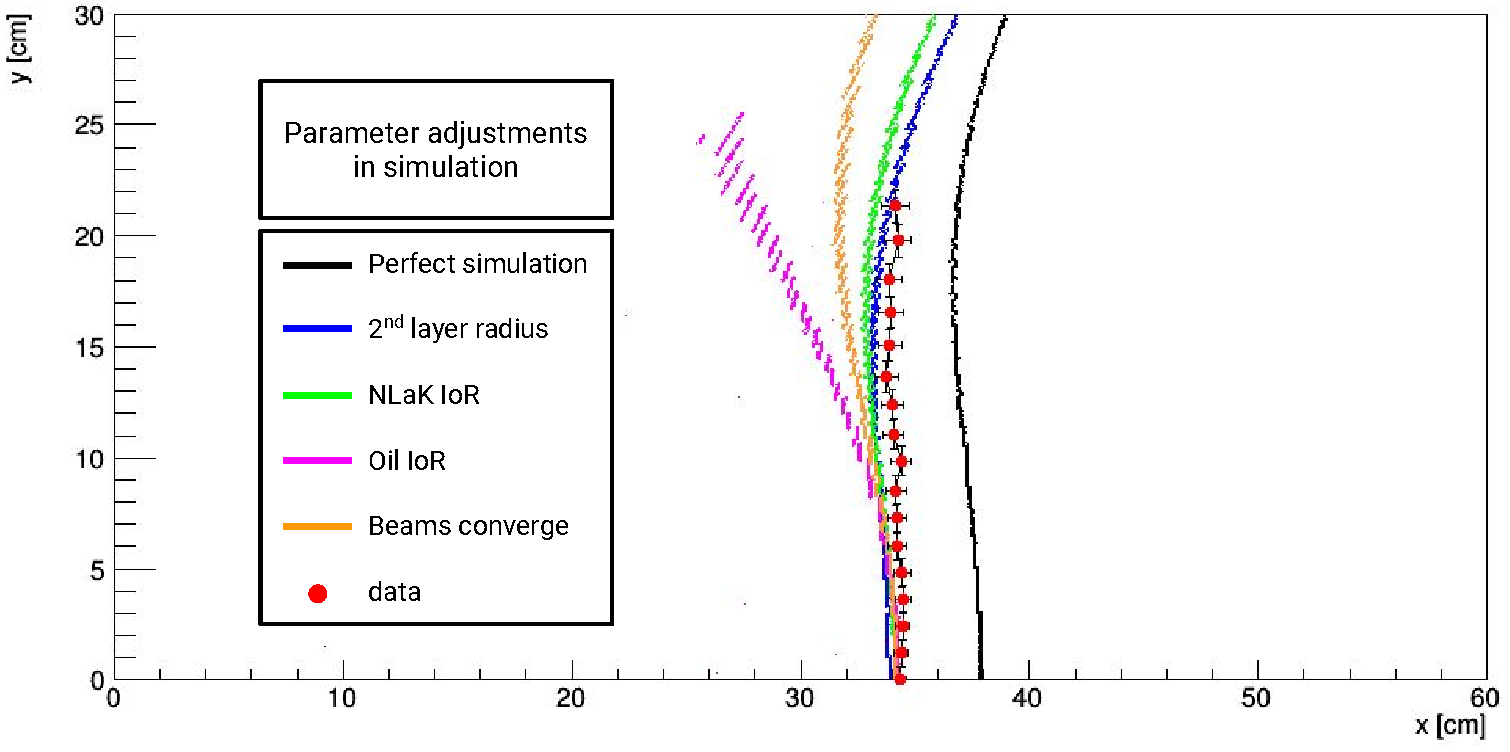
\includegraphics[width=\textwidth]{focal_plane_shifts_together.pdf}
	\caption{Shifting the focal plane of the GEANT4 simulation: decrease the radius of the second layer by $1.3$~mm (blue), increase the refractive index of NLaK33 by $0.03$ (green), decrease the index of refraction of the mineral oil by $0.15$ (pink), and give a converging angle of the laser beams of $0.15$~mrad (black). Experimental data is shown in red and simulation with ``perfect" parameters is shown in black.}
	\label{fig:focal_plane_shifts}
\end{figure}

\begin{figure}[!htb]
	\centering
	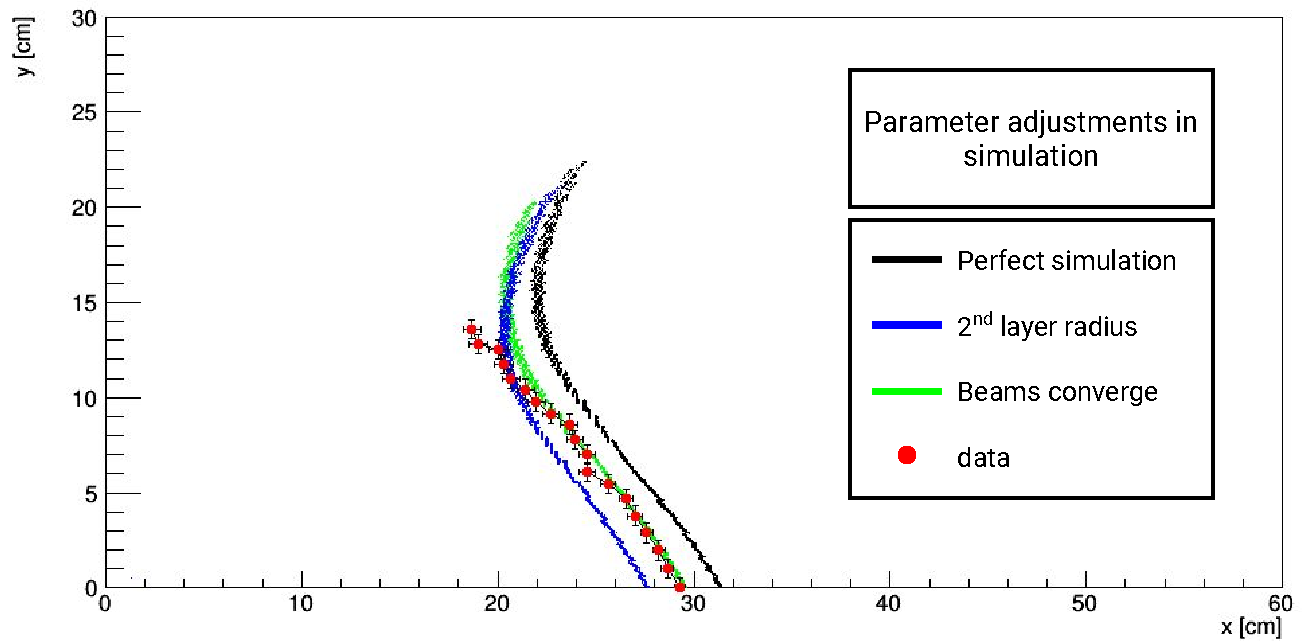
\includegraphics[width=\textwidth]{focal_plane_xshift.pdf}
	\caption{Focal plane after implementing a $7$~mm shift along a line connecting the two beams for data (red) and simulation assuming ``perfect" parameters (black), a reduction in the radius of the second curved surface (blue), and a non-parallelism between the beams (green). Clearly the modification of the radius overcompensates for the change in the position and shape of the focal plane while the non-parallelism assumption agrees very well.}
	\label{fig:focal_plane_xshift}
\end{figure}

%----------------------------------------------------------------------
%	NLAK33 RAD HARDNESS SECTION
%----------------------------------------------------------------------

\clearpage
\section{Radiation Hardness of NLaK33}
Fused silica, which is used for most of the optical components in all current DIRC designs, was already extensively tested in the BaBar and PANDA experiments \cite{RadHardness} and has proven to be radiation hard up to several hundred krad with little to no loss of transmission. The determination of the radiation hardness of NLaK33 is an important study for the EIC R\&D program. 

The irradiation of a pure sample of NLaK33 material was performed at Catholic University of America (CUA) in a Faxitron CP-160 Cabinet X-Radiator System \cite{XRayCabinet} (Figure \ref{fig:x-ray_setup}a). The cabinet allows for a minimum of 6 second X-ray exposure. Photon energy was set to 160 keV with a 6.2 mA current for all exposures of the NLaK33 sample.

A RaySafe ThinX RAD dosimeter \cite{Dosimeter}, shown sitting on the X-ray cabinet shelf in Figure \ref{fig:x-ray_setup}b, was used to measure the radiation dose being delivered to the sample. Unfortunately the exposure time of the dosimeter is limited to less than 10 seconds, so the shortest time setting on the X-ray cabinet was used. This exposure time of 6 seconds was found to be closer to 7.5 seconds by the dosimeter due to rise and fall time of the source. This shortest exposure time consistently gave readings of 81.4 rad. The dosimeter has a circular active area of $706.9\unit{mm}^2$ while the side of the NLaK33 sample that was exposed to the source has an area of $8\times28\unit{mm}^2$, so the dose delivered to the sample is approximately 25 rad.

To measure the transmission of the sample a LAMBDA 950 UV/Vis/NIR Spectrophotometer \cite{Monochromator} (Figure \ref{fig:monochromator_setup}a), referred to from here on as a monochromator, was used. The monochromator has a dynamic range between 175 - 3,300 nm wavelength in 1 nm steps. The sample of NLaK33 was held in place using an optics stand (Figure \ref{fig:monochromator_setup}b) to make sure measurements were consistent and reproducible. Measurements of the transmission of the sample were taken between each set of radiation exposures. The transmission of sample of fused silica was also tested between each radiation exposure of the NLaK33 sample, but was only used as a control sample and was found to be stable.

Because it was not clear exactly what percentage of the total dose read by the dosimeter was from the warm up and cool down of the cabinet it was decided that the best approach for exposure of the sample was to do multiple steps of the 6 second exposure time and record the accumulated dose in this manner. The first exposure was 4 intervals for a total of 100 rad. After this measurement it was noticed that there was already a roughly 2\% drop in the transmission of the sample at 420 nm wavelength \footnote{420~nm wavelength was chosen because it is near the peak of the quantum efficiency of the multi-channel plate photomultiplier tubes discussed later in this chapter and used in the analysis presented in Chapter \ref{ch:analysis}}, so steps of 50 rad were taken for the next several measurements. After 700 rad of dose it was clear that there was a linear correlation between accumulated dose and loss in transmission, so it was decided that 100 rad steps could again be taken. 

Results for the radiation hardness tests of the NLaK33 sample are shown in Figure \ref{fig:transmission_measurements}. The transmission loss below roughly 350~nm wavelength and above 700~nm wavelength seems to be negligible. However, in the range of 350-700~nm there is a clear dip in transmission. At 420~nm wavelength, corresponding to the peak in the quantum efficiency of the photodetectors used in the DIRC, sees a 1.3\% drop in transmission per 50 rad of dose. While it is not yet clear what the expected integrated dose will be in the area of the DIRC at the EIC it is assumed that this loss is too great over the lifetime of the detector. Other materials known to be radiation hard, such as lead fluoride, are being investigated as possible alternatives.

\begin{figure}[!htb]
	\centering
	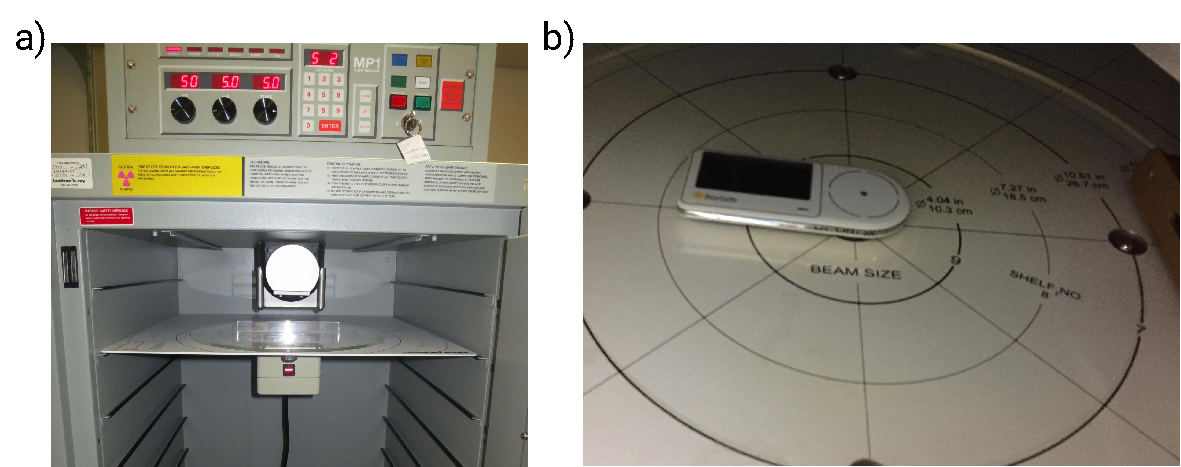
\includegraphics[width=\textwidth]{x-ray_setup.pdf}
	\caption{The Faxitron CP-160 Cabinet X-Radiator System (a) used to irradiate the NLaK33 sample with 160 keV photons at 6.2 mA current for 6 second intervals, and the RaySafe ThinX RAD Dosimeter (b) sitting on one of the X-ray cabinet shelves.}
	\label{fig:x-ray_setup}
\end{figure}


\begin{figure}[!htb]
	\centering
	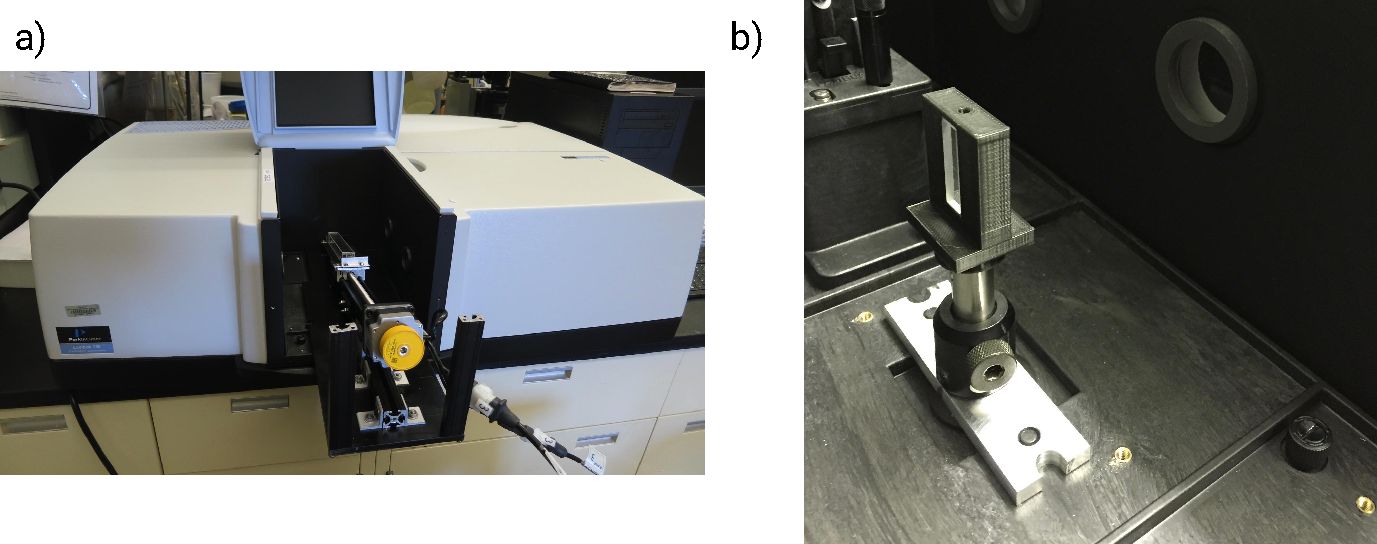
\includegraphics[width=\textwidth]{monochromator_setup.pdf}
	\caption{The LAMBDA 950 UV/Vis/NIR Spectrophotometer (a) and a closeup view of the NLaK33 sample being held in position by the optics stand (b).}
	\label{fig:monochromator_setup}
\end{figure}

\begin{figure}[!htb]
	\centering
	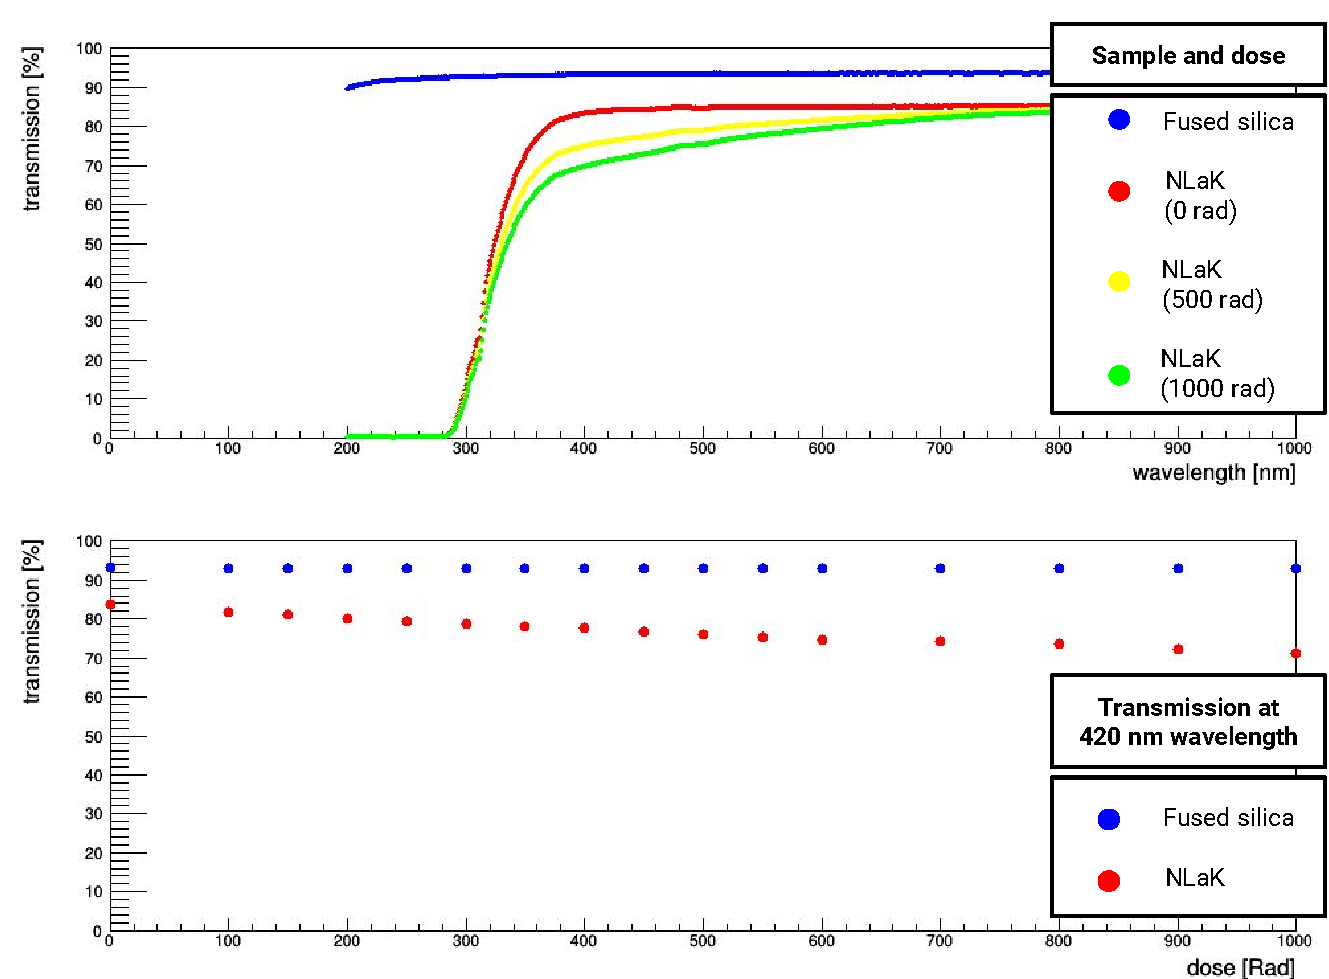
\includegraphics[width=\textwidth]{transmission_measurements2.pdf}
	\caption{The top plot shows the transmission of the control sample of fused silica (blue) and the transmission of the NLaK33 sample after 0 (red), 500 (yellow), and 1000 (green) rad dose across a range of 200-800 nm wavelength. The bottom plot shows the transmission of the NLaK33 sample at 420 nm wavelength as a function of the dosage. After the first 700 rad of dose it was clear that there was a linear relationship between dose and transmission loss, so 100 rad steps were used afterwards.}
	\label{fig:transmission_measurements}
\end{figure}

%----------------------------------------------------------------------

%	HIGH-B TESTS SECTION
%----------------------------------------------------------------------
\clearpage
\section{Performance of MCP-PMTs in High Magnetic Field}
The limiting space requirements of the EIC DIRC design, as mentioned in Chapter \ref{ch:eicdirc}, places a unique set of requirements on the DIRC readout sensors. In order to achieve the desired single photon resolution while maintaining a sufficiently sized expansion volume the sensors, and therefore the pixels, must be compact. Furthermore, due to the positioning of the readout plane inside the large field of the solenoid magnet (see Figure \ref{fig:jleic_layout}) these sensors must also have a high tolerance to magnetic fields, both in magnitude (up to 3 T or higher), non-uniformity, and orientation. Ordinary photomultiplier tubes (PMTs) are not an option due to their susceptibility to magnetic fields, being affected by fields as small as 0.5 Gauss \cite{PMT_magnet}. Silicon photomultipliers (SiPMs) are attractive due to their very compact size and their resistance to magnetic fields up to 4 T \cite{SiPM_characterization}. However, the inherent background, or dark count, of SiPMs is very large, on the order of MHz per pixel \cite{SiPM_characterization} \cite{HamamatsuSiPM}. Because a DIRC detector only expects 100 photons per event at most spread over $100$~ns, this level of background is far too large for usability. The dark noise can be mitigated by cooling, with a decrease by a factor of approximately 2 per $5^\circ$~C, but the large amount of cooling required around the SiPMs in the EIC detector would be costly both in space and finance. With these requirements in mind the best option for an EIC DIRC detector is the use of micro-channel plate photomultiplier tubes (MCP-PMTs) (Figure \ref{fig:MCP_schematic}). The dark count of MCP-PMTs is on the order of kHz \cite{MCPPMT_darkcount}, which is much more acceptable compared to SiPMs. MCP-PMTs also have a much higher resistance to external magnetic fields than traditional PMTs due to the small pore size, with studies being done up to 2 T \cite{MCPTest1}, \cite{MCPTest2}, \cite{MCPTest3}, \cite{MCPTest4}, \cite{MCPTest5}, \cite{MCPTest6}. The tests described below are the first to study the effects of fields as large as 5 T on MCP-PMTs.

\begin{figure}[!htb]
	\centering
	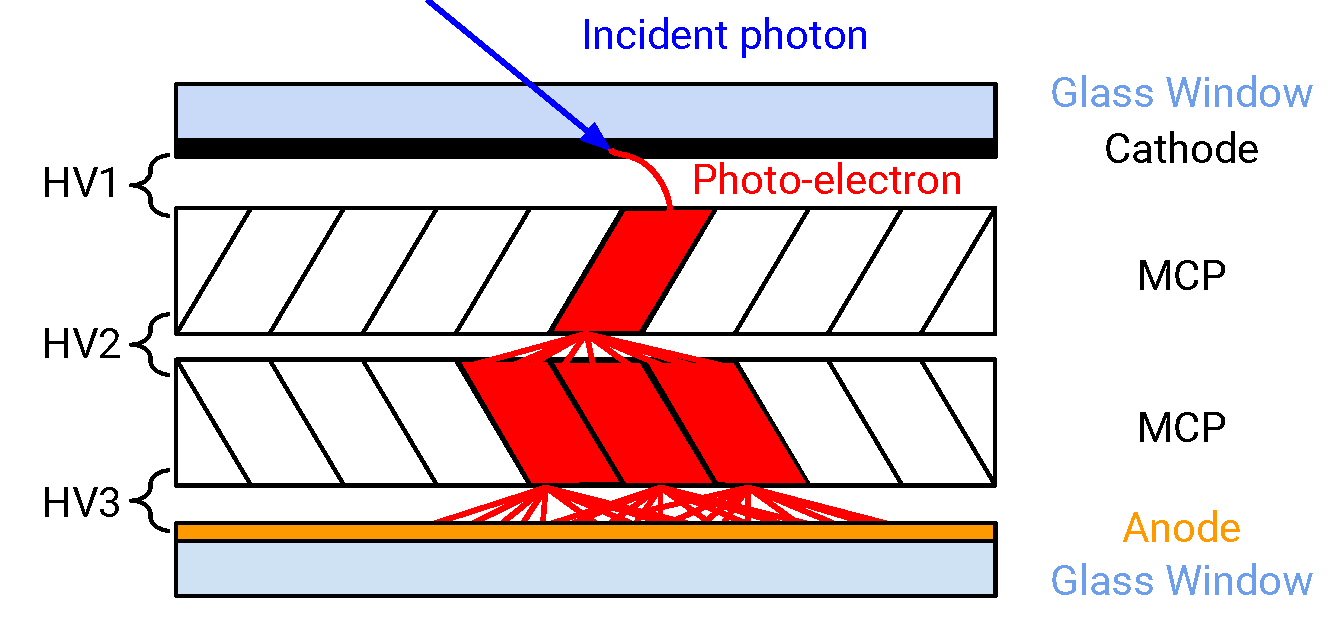
\includegraphics[width=\textwidth]{MCP_schematic.pdf}
	\caption{Schematic of the Micro-channel Plate photo-multiplier tube (MCP-PMT) concept. A cathode and anode sandwich two conducting plates with micrometer-sized channels (MCP), and a high-voltage (HV) difference (HV1, HV2, HV3) between every two components. The channels, or pores, of the two MCPs are aligned in a chevron pattern. An incident photon (blue) strikes the cathode, producing a photo-electron (red). That electron is accelerated through the potential difference between the cathode and first MCP (HV1) before striking the inside of one channel. This creates the same effect as an electron striking the dynode of a typical PMT, resulting in an avalanche of photo-electrons that emerge out of the other side of the first MCP. These electrons are again accelerated through a second potential difference (HV2) before repeating the process in the second MCP. Finally, the copious photo-electrons exit the second MCP, are accelerated through a final potential difference (HV3), and are collected on the anode. This design is both much more compact, more resistant to magnetic fields compared to traditional PMTs, and has less timing jitter. }
	\label{fig:MCP_schematic}
\end{figure}

\subsection{Experimental Setup}
In the fall of 2014 two single-anode MCP-PMTs were tested at Jefferson Lab \cite{HighB_DIRC2015}, a PHOTONIS PP0365G ($6 \mu\text{m}$ pore size and a $18.2 \unit{mm}$ active area) \cite{PHOTONIS} and a Photek PMT210 ($3 \mu\text{m}$ pore size and a $10 \unit{mm}$ active area)  \cite{Photek}, shown in Figure \ref{fig:highB_magnet} at the top and bottom right respectively. The FROST  superconducting solenoidal magnet, with a field tunable up to 5 T with a cylindrical bore diameter of 12.7 cm and a length of 76.2 cm, was used for testing \cite{JLab_FrozenTarget}. The central field of the magnet, while quite large, is also very homogeneous, with an inhomogeneity of less than $5\times10^{-5}$ over a cylindrical volume with a diameter of 1.5 cm and a length of 5 cm. The sensors were held in place at the center of the magnet using a custom-built, non-magnetic, light-tight cylindrical dark box, as shown in Figure \ref{fig:highB_magnet}. Inside the dark box the sensor was held in place by a turn table that allowed for rotation around a vertical axis as well as a horizontal axis (the Y(Y') and Z(Z') axes in Figure \ref{fig:highB_schematics} respectively). The range of the polar angle $\theta$ was dependent on the size of the sensor being measured as well as the signal and HV cables connected to the back of the sensor. A cart allowed the sensor to move relative to the dark box for precise positioning at the center of the magnet. The gain of both sensors were scanned for various angles of $\theta$, $\phi$, and a range of magnetic field from 0 to 5 T.

A pulser-driven LED was used to illuminate the MCP-PMTs with 470 nm photons. An optical fiber was used to transmit the photons to the dark box and a diffuser installed inside the dark box cap was used to illuminate the entire face of the sensor with nearly constant intensity and 10 ns wide pulses at 30 kHz. The sensor signal output was then amplified using a 200-times preamplifier and used as input to a 250~MHz flash analog-to-digital converter (fADC) with 4096 sample depth provided by the JLab Electronics Group. The fADC was then read out by our data acquisition system (DAQ).The pulser was also used as the trigger signal for the fADC, as shown in the chart in Figure \ref{fig:highB_schematics} (right).

My contribution to these studies was assisting in the experimental setup, data monitoring and collection, restructuring and updating the signal reconstruction software, and operating the FROST magnet and electronics both during and between runs. The analysis of the data was done by Dr. Yordanka Ilieva from the University of South Carolina, who's results are shown below and taken, with permission, from \cite{HighB_DIRC2015}.


\begin{figure}[!htb]
	\centering
	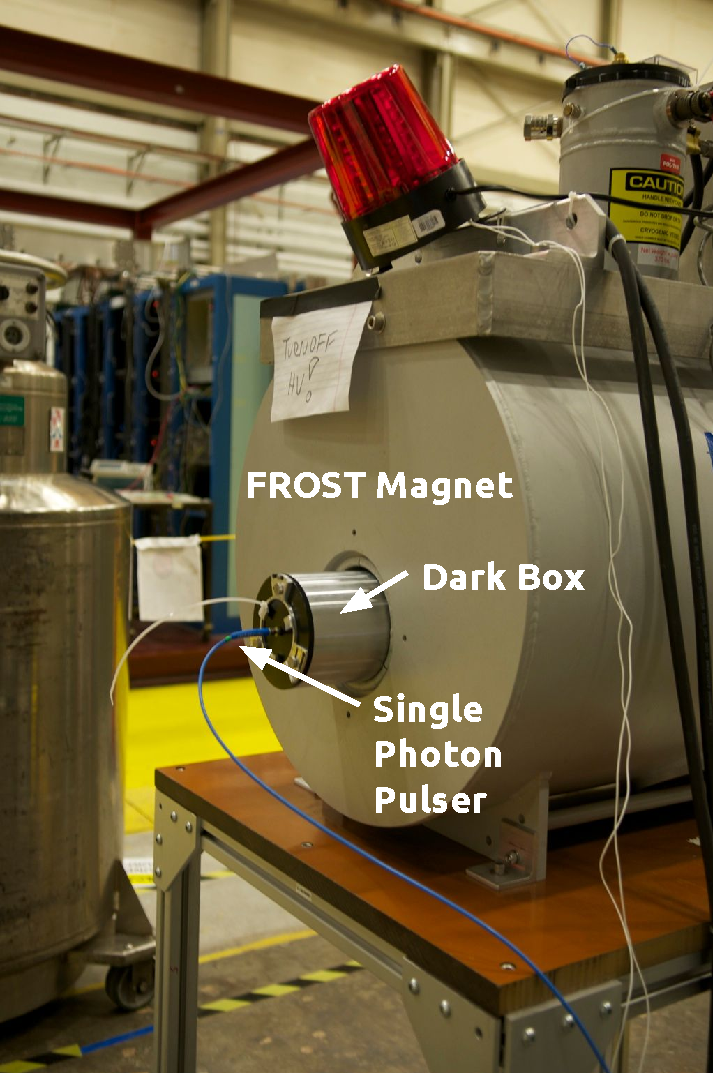
\includegraphics[width=0.8\textwidth]{highB_magnet.pdf}
	\caption{The FROST superconducting magnet (left) with the dark box placed in the bore, and the Photek PMT210 (top right) and PHOTONIS PP0365G (bottom right) MCP-PMTs used for testing at JLab.}
	\label{fig:highB_magnet}
\end{figure}

\begin{figure}[!htb]
	\centering
	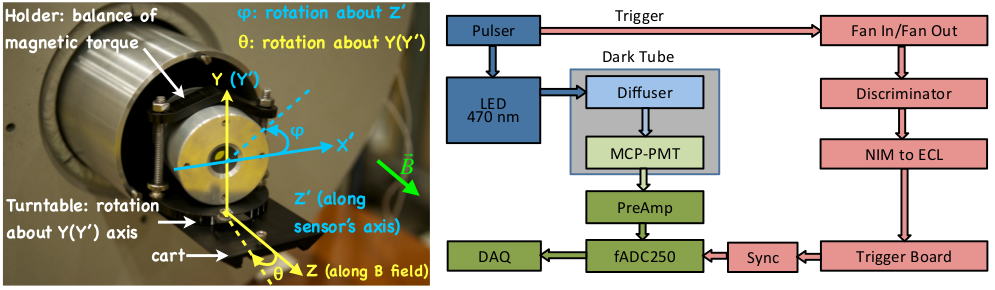
\includegraphics[width=\textwidth]{highB_schematics.png}
	\caption{Left: A closeup of the dark box showing the Photek PMT210 being held in place by the turn table. This setup allows the MCP-PMT to be rotated around both the horizontal Z(Z') axis as well as the vertical Y(Y') axis (with respect to the floor). The rotation about the Y(Y') and Z(Z') axes are described by the polar angle $\theta$ and azimuthal angle $\phi$ respectively. The magnetic field is parallel to the central axis of the dark box. Right: A flowchart of the readout used for testing. The photocathode is exposed to single 470 nm photons to produce photoelectrons, with a large voltage difference between the anode and cathode used to create an avalanche. The total charge is collected on the anode, amplified by a preamplifier, and digitized by an fADC and read out by a DAQ. \cite{HighB_DIRC2015} }
	\label{fig:highB_schematics}
\end{figure}

\subsection{Results}
The gain of the sensors is proportional to the average charge per pulse collected on the sensor anode, and thus the performance can be measured in terms of the average charge collected on the fADC. This is calculated by taking the integral of the fADC signal. The fADC samples the signal every 4 ns in a $1 \mu\text{s}$ window. For each event, $i$, the average pedestal was determined from the fADC using the first 20 bins, and the waveform is integrated over 9 bins around the peak. The integral of the pedestal is subtracted, resulting in a value, $Q_{9,i}$, that is proportional to the total charge collected on the anode for that event. The average values of $Q_{9,i}$ for each setting of field, $\theta$, and $\phi$ are used in the results presented. Figure \ref{fig:highB_waveform} (left) shows an example of a waveform from the PP0365G sensor. Another strategy used for calculating the collected charge was to integrate the entire pedestal-subtracted average waveform (Figure \ref{fig:highB_waveform} right). This yielded results consistent with the event-by-event analysis.

Figure \ref{fig:highB_nominal_HV} shows the performance of both sensors at the nominal ($\theta = \phi = 0^{\circ}$) position for magnetic fields up to 5 T. Data were taken for HV settings of 93\% (black) and 97\% (red) of the maximum manufacturer-recommended HV value. The PP0365G sensor shows a smooth, nearly linear decrease in charge as the field increases, being able to operate at up to 3 T with a factor of 15 loss in collected charge. By increasing the HV the operational range was extended to 3.5 T. The PMT210 has an increase in the collected charge up to 0.5 T with a smooth decrease thereafter as the magnitude of the field increases, staying operational until 4 T with only a factor of 6 decrease in collected charge. Increasing the HV allowed signal to be collected up to 5 T. An uncertainty of 5\%, shown in the error bars of each data point, was the dominant source of error, with the systematic uncertainty giving less of a contribution. The latter was estimated as the standard deviation of the sample of repeated outcomes of the average collected charge at the same setting (mainly the nominal angle setting at a 0 T field) from runs taken randomly throughout the measuring period. The standard deviation acccounts for the variations of the light intensity on the photocathode and of the positioning of the sensor in the dark box.

Figure \ref{fig:highB_QBtheta} shows the response of the sensors at various $\theta$ angles up to $30^{\circ}$. As one can see, the two sensors have very different responses. The magnetic field dependence of the collected charge for the PP0365G shows a maximum below 1 T for $\theta = 20^{\circ}$, $25^{\circ}$, and $30^{\circ}$, while $\theta = 0^{\circ}$ and $10^{\circ}$ show a smooth decrease as magnetic field increases. There is also a much more rapid decrease in collected charge at fields above 1 T for higher angles. The PMT210, however, shows a more uniform characteristic for all $\theta$ angles. For both sensors, as the $\theta$ angle increases the field range in which the sensor can reliably operate becomes more narrow.

The effect of changing the $\phi$ angle of the PP0365G sensor for different magnetic field strengths and $\theta$ angles of $10^{\circ}$ and $20^{\circ}$ can be seen in Figure \ref{fig:highB_QBphi}. Because the outer casing of the sensor is cylindrical and there is no apparent orientation, a $\phi = 0^{\circ}$ position was chosen randomly and marked on the front of the casing for consistency. The rotation was done counterclockwise about the sensor's axis when looking from the front. The data shows that at a fixed $\theta$ angle the collected charge has a $\phi$ dependence, and this dependence is strongly correlated to the $\theta$ angle. The larger $\theta$ angle shows a much faster decrease in collected charge as the $\phi$ angle increases.

\begin{figure}[!htb]
	\centering
	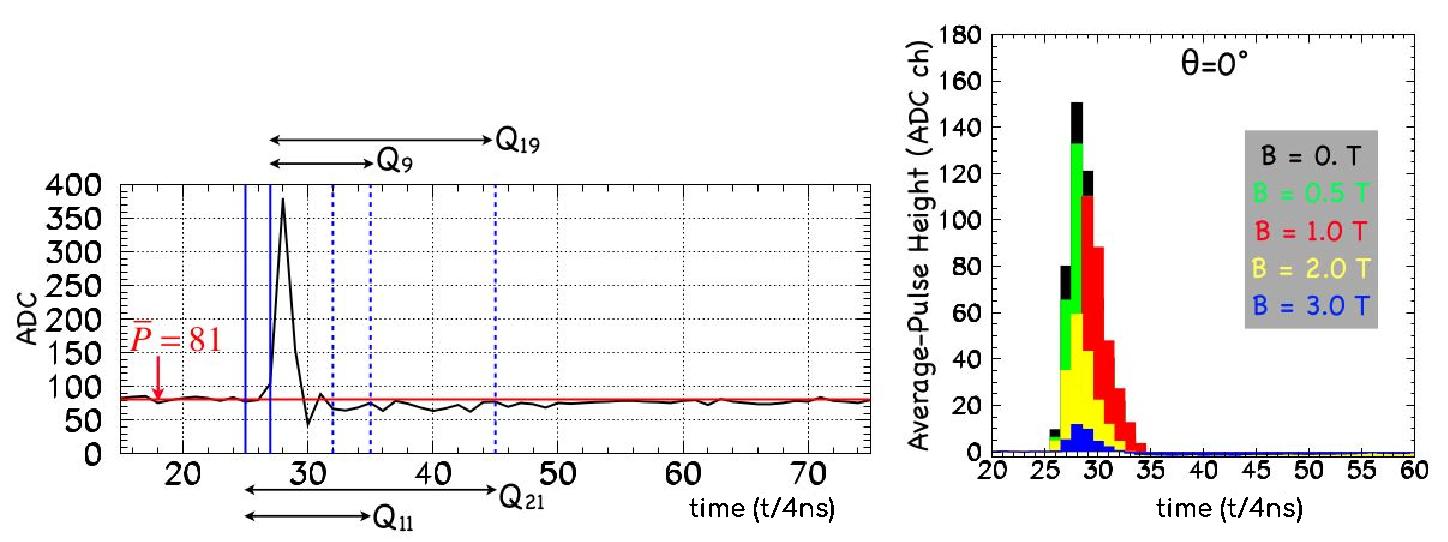
\includegraphics[width=\textwidth]{highB_ADCintegration.pdf}
	\caption{Left: an example waveform measured for the PP0365G sensor. Each bin of the x-axis corresponds to a 4 ns interval. The y-axis is the fADC value (ranging from 0 to 4096). The solid red line shows the calculated pedestal position for the event. The ranges $Q_9$, $Q_{11}$, $Q_{19}$, and $Q_{21}$ denote the positions of integration ranges over 9, 11, 19, and 21 bins respectively for calculation of the total anode charge for that event. The limits and width of the integration range were varied for systematic purposes. Right: the average waveforms of the PP0365G sensor at $\theta = 0^{\circ}$ and varying magnetic field strengths. There is a clear negative correlation between the signal amplitude and field magnitude.}
	\label{fig:highB_waveform}
\end{figure}

\begin{figure}[!htb]
	\centering
	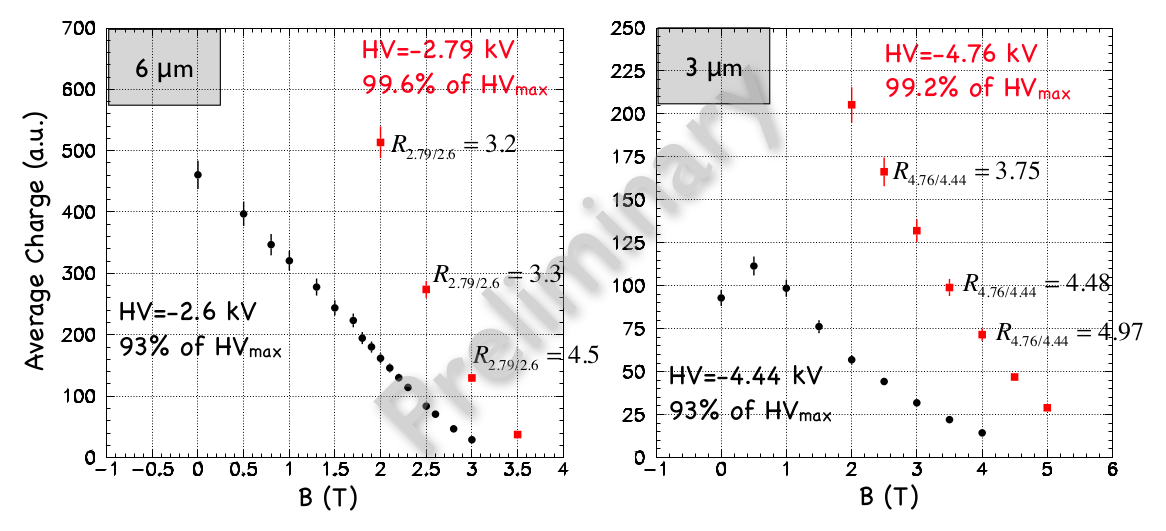
\includegraphics[width=\textwidth]{highB_QBV.png}
	\caption{The gain performance of the PP0365G and PMT210 sensors (left and right) at $\theta = 0^{\circ}$ and two HV settings. The black and red points were measured using 93\% and 99\% of the maximum manufacturer recommended HV (HV\textsubscript{max}) settings respectively. For the PP0365G at 93\% (95\%) of HV\textsubscript{max} a reasonable signal can be obtained up to a 3 (3.5) T field, though the total collected charge decreased by a factor of 15 when going from 0 T to 3 T. The PMT210 was able to produce a signal at fields up to 4 (5) T, and the collected anode charge decreased only by a factor of 6 when going from 0 to 4 T. The error bars on all points include both statistical and 5\% systematic uncertainties, with the latter being the dominate contribution.}
	\label{fig:highB_nominal_HV}
\end{figure}

\begin{figure}[!htb]
	\centering
	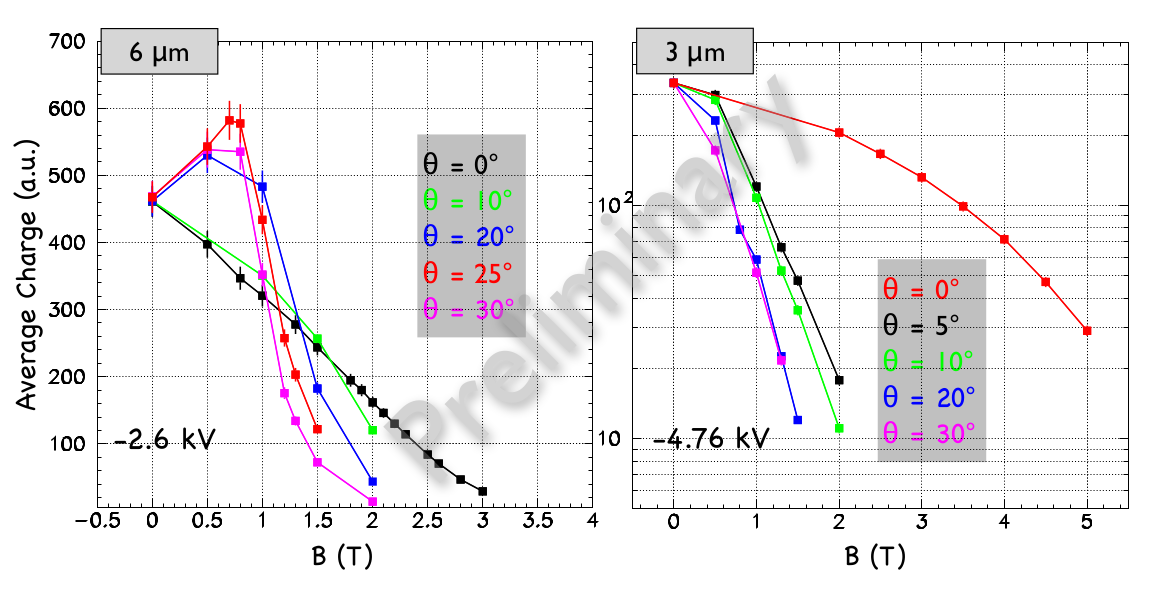
\includegraphics[width=\textwidth]{highB_QBtheta.png}
	\caption{The average collected anode charge as a function of magnetic field strength at various $\theta$ rotation angles for the PPP0365G (left) and PMT210 (right) sensors.}
	\label{fig:highB_QBtheta}
\end{figure}

\begin{figure}[!htb]
	\centering
	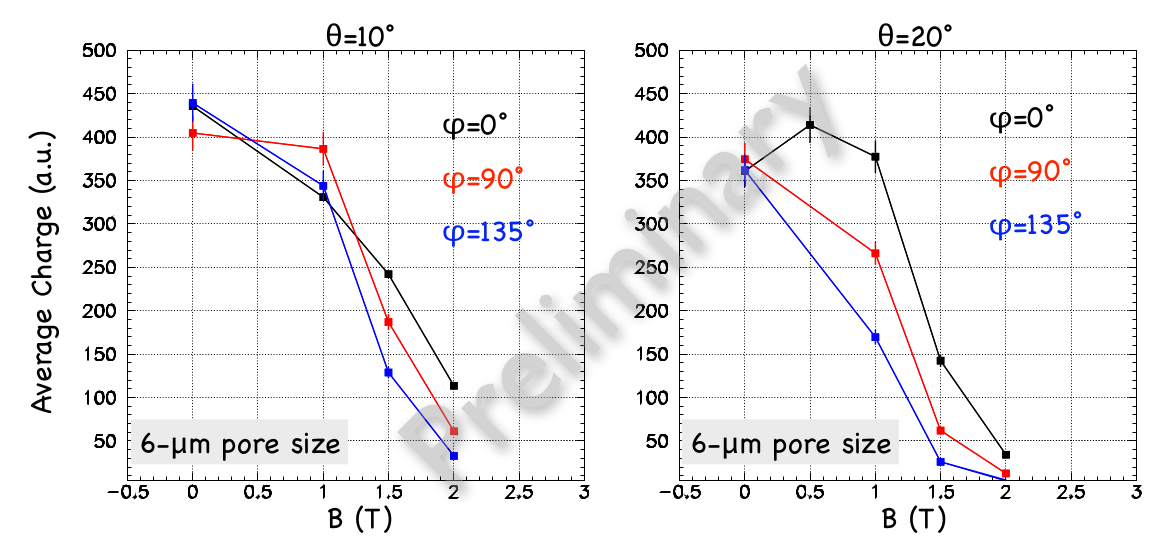
\includegraphics[width=\textwidth]{highB_QBphi.png}
	\caption{The average collected anode charge as a function of magnetic field strength at various $\phi$ rotation angles for the PP0365G at fixed $\theta$ angles of $10^\circ$ (left) and $20^\circ$ (right).}
	\label{fig:highB_QBphi}
\end{figure}

\subsection{Conclusions}
Overall the data at $\theta = 0^{\circ}$ suggests that a smaller pore-size sensor (PMT210) has a higher resistance to the effects of high magnetic fields as it was able to operate up to 5 T fields and had a slower decrease in collected charge with increasing field than the PP0365G sensor. The smaller pore-size sensor as showed an higher increase in collected charge with increased HV. When increasing the $\theta$ angle, however, the PMT210 showed a much more rapid decrease in performance compared to the PP0365G. At $0^{\circ}$ the PMT210 can be operated up to 5 T, while rotating to $5^{\circ}$ there is a dramatic decrease in maximum field to 2 T. The PP0365G sensor, however, was more stable with rotations in $\theta$, dropping from 3 T at $0^{\circ}$ to 2 T at larger angles.

While the data for the two sensors allow to make general conclusions about the effect of pore size on performance, more detailed conclusions cannot be made with certainty as the orientation of the MCPs inside the sensors are not necessarily the same. While the definition of the $\theta$ angle is consistent for both sensors in this testing, the azimuthal orientation of the channels relative to the central axis may differ greatly. No details are given by the manufacturer about the absolute azimuthal orientation of the channels for each sensor as this information has not as of yet been necessary for applications of MCP-PMTs. These data, however, suggest that this will be important for optimization of the sensor design and operational parameters for operations in areas of non-homogeneous, high-strength magnetic fields, such as for the EIC DIRC.
 % testing lens focal plane and rad hardness, and MCP-PMTs
%
\chapter{3-Layer Lens Performance in Particle Beam}
\section{Prototype Setup}
\section{Simulated Performance}
\section{Data Analysis}
\subsection{Error Evaluation} % analysis results from CERN 2015 test beam
%
\chapter{Outlook and Summary}
%----------------------------------------------------------------------
%	SUMMARY CHAPTER
%----------------------------------------------------------------------
\label{ch:summary}

\section{Results}
A DIRC detector is ideal for meeting the hadronic PID requirements in the barrel region of an EIC due to its small radial footprint and excellent particle separation capabilities at sub-10~GeV/c particle momentum. The current baseline design of the EIC DIRC is based on the compact PANDA DIRC design \cite{PANDA_barrel}, featuring a compact expansion volume and lens-based focusing. Both geometric and time-based reconstruction analysis were done on the GEANT4 simulation of the EIC DIRC. For the geometric reconstruction Figure \ref{fig:EIC_track_res} shows a reasonable performance that would allow for $3\sigma$ $\pi/K$ separation (see Figure \ref{fig:PID_performance} for reference) at 6~GeV/c momentum for most polar angles and dropping only slightly below $3\sigma$ if it is assumed that a large correlated term of 1~mrad will be seen in the actual experiment. In the case of the time-based reconstruction (Figure \ref{fig:EIC_timebased_performance}) the simulation again predicts a $3\sigma$ separation for a majority of the polar angle range of the detector, with performance dropping for polar angles near perpendicular.

While it would be ideal to test these simulation results directly with physical measurements, at this stage of the R\&D effort it is more sensible to take advantage of the synergy between the EIC DIRC group and other DIRC groups rather than spend some large fraction of the PID R\&D budget on a single EIC DIRC prototype. A synergistic test beam campaign was carried out during the summers of 2015 and 2016 with the PANDA Barrel DIRC group to study the performance of a PANDA DIRC detector prototype using the components envisioned for the EIC DIRC, namely a new 3-layer lens focusing optic designed to have a flat focal plane across the face of the MCP-PMT detector plane. Verification that the GEANT4 simulation using this PANDA prototype geometry agrees with experimental data is key in ensuring that the predicted performance of the EIC DIRC is valid.

Along with the analysis of the performance of the EIC DIRC 3-layer lens in a particle beam, it was also necessary to investigate the radiation hardness of the center layer of lanthanum crown glass \cite{SchottData}, NLaK33, as well as the actual shape of the focal plane to compare with simulation. Measurements of the radiation hardness were carried out at the Catholic University of America using  160~keV X-ray cabinet \cite{XRayCabinet} for irradiation and a monochromator \cite{Monochromator} for measuring the transmission of the glass after each irradiation step. It was found that the glass suffers approximately 1.3\% transmission loss per 100~rad of delivered dose (Figure \ref{fig:transmission_measurements}). It is, at the time of this writing, unknown what the expected dose delivered to the DIRC detector at an EIC will be over the lifetime of the experiment. Alternatives and solutions are discussed in the next section.

Measurements of the focal plane of the 3-layer lens were done at Old Dominion University using a custom-built laser setup and 3D printed lens holder. Initial measurements showed a systematic shift in the position of the focal plane between data and simulation by roughly 4~cm. After many measurements and adjustments to the setup it was found that the cause of this shift was most likely due to a non-zero angle between the two laser beams of roughly 0.15~mrad. After this adjustment was implemented in the simulation, the measured data very nicely reproduces both the shape and position of the predicted focal plane for multiple tilt angles and even when shifting the beam off-center of the lens.

The analysis of the 2015 CERN test beam data from the PANDA DIRC prototype focused primarily on the configuration with the 3-layer lens, bar radiator, and 7 GeV/c beam momentum in an attempt to closely match the parameters of the EIC DIRC baseline design. Both the geometric and time-based reconstruction methods were used to determine the performance of the prototype. The GEANT4 simulation is in good agreement with the results of the analyzed experimental data, which gives confidence to the results presented in Chapter \ref{ch:eicdirc} for the EIC DIRC that the desired PID performance can be achieved by such a detector. 

Confirmation that the GEANT4 simulation package for the EIC DIRC agrees with physical data is crucial in proceeding with the R\&D effort. A synergistic test beam campaign was carried out with the PANDA Barrel DIRC group from GSI at CERN in the summer of 2015 using a prototype detector modeled after the baseline design of the PANDA DIRC. During the 2015 CERN test beam campaign multiple configurations of beam momentum, radiators, and focusing optics were tested (see Table \ref{tab:runs2015}). Study 151, using the 3-layer lens, a bar radiator, and 7 GeV/c beam momentum, was used in the main analysis for this thesis due to its similarities to the baseline design of the EIC DIRC. Both the geometric and time-based reconstruction methods were used to determine the performance of the prototype. The GEANT4 simulation is in good agreement with the results of the analyzed experimental data, which gives confidence to the results presented in Chapter \ref{ch:eicdirc} for the EIC DIRC that the desired PID performance can be achieved by such a detector. 

\section{Future Work}
There are still several steps to take in the R\&D effort for the EIC DIRC: further studies of the radiation hardness of NLaK33, alternative materials for the lens design, and building a full, baseline-design-compatible EIC DIRC prototype.

Tests of the radiation hardness of NLaK33 were done with a somewhat thick (1~cm) piece of glass. The central layer of the 3-layer lens design, however, is set to 0.56~cm at the thickest portion, and thins out to 0.2~cm at the edge (see Figure \ref{fig:3CS_schematic}). It is unclear what the penetration depth of NLaK33 is, and therefore how big of a change a smaller volume of material would have on the transmission. Talks are currently underway with a manufacturer to procure a piece of glass with a smaller thickness to test the penetration depth.

Along with testing the penetration depth of NLaK33, tests are also planned for exposing the material to neutron radiation. Again, the neutron flux at the DIRC detector in an EIC is unclear, but having a feel for the type of neutron damage the material can withstand will help in the development of the lens.

If, after all radiation tests of the thinner NLaK33 piece are complete, it is found that it will lose as significant amount of transmission after a relatively short time of running then an alternative material must be found for the lens. Currently there are investigations into making the lens out of a different material called Lead fluoride (PbF$_2$). PbF$_2$ is ideal because of its high refractive index, similar to that of NLaK33, and its proven high radiation hardness \cite{PbF2RadHard}. The challenge with using PbF$_2$ in the lens is that many manufacturers are unwilling to work with it due to the fear of contamination of their tools with lead.

In order to fully test the EIC DIRC design a prototype must be constructed and tested in a hadron beam. To carry out such a test beam campaign, MCP-PMTs with appropriately sized $3\times3\unit{mm}^2$ pixels (crucial for the desired resolution) along with a correctly sized expansion volume and radiator bars must be procured. Costs can be somewhat mitigated if radiator bars from previous experiments could be used instead of purchasing new bars. It is currently planned to include the costs of a full test beam in the US as part of the 2019 EIC budget for detector R\&D.

In conclusion, a DIRC detector is an ideal solution for hardronic PID in the barrel region around the electron/ion interaction point of an EIC due to its compact radial size and resolving power for charged particles with sub-10~GeV/c momentum. Many milestones have so far been achieved in the R\&D efforts, including the verification of the EIC DIRC simulation package via the 2015 CERN test beam, confirmation of the shape of the new 3-layer spherical lens design at ODU, limited radiation hardness testing of the NLaK33 material at CUA, and extensive studies of the influence of high magnetic fields on MCP-PMTs at JLab.  % outlook of future work and summary of results

  %This begins the list of reference or bibliography.
  %The default form is consistent with the references in the Physical Review.
  %The articles must be listed in the order in which they appear in the text.
  %The style of the bibliography can be changed and automatic ordering of the entries can be accomplished using BibTeX.
  %Use of BibTeX is explained in most of the standard LaTeX books.

\addcontentsline{toc}{chapter}{BIBLIOGRAPHY}  %This command adds and entry for the bibliography in the table of contents

\bibliography{bibliography}{}
\bibliographystyle{unsrt}

%A new command for appendix chapters has been defined called \achapter that has been modified
%so that it can add the appendices to the table of contents in the approved form.

\appendix

\achapter{Error Evaluation}

\newpage

%The command below initiates printing of the vita page. The name and other information is taken from previous entries.

\vitapage


\end{document}
